% =========================================================================
% Diseno y caracterizacion de aleatoriedad de un TRNG basado en
% osciladores en anillos -- VERSION EN ESPANOL (de lectura)
%
% Traduccion de tfm_main.tex y chapters/*.tex, que siguen siendo la
% version de referencia mientras no se confirme con los tutores el idioma
% de la entrega. Los capitulos traducidos estan en chapters_es/; las
% etiquetas (\label), citas y figuras son las mismas que en la version
% inglesa. Al cambiar un capitulo en ingles hay que trasladar el cambio
% aqui.
%
% Master Universitario en Microelectronica: Diseno y Aplicaciones de
% Sistemas Micro/Nanometricos. Universidad de Sevilla / IMSE-CNM-CSIC,
% curso 2026-2027. Autor: Mario Garcia Jimenez.
% Compilar: pdfLaTeX + BibTeX (fichero principal: tfm_main_es.tex)
% =========================================================================
\documentclass[12pt, a4paper, oneside]{report}

\usepackage[utf8]{inputenc}
\usepackage[T1]{fontenc}
% es-noshorthands: los atajos de < > del espanol rompen TikZ.
% es-nodecimaldot: los decimales en modo matematico se escriben {,}.
\usepackage[spanish,es-tabla,es-noshorthands,es-nodecimaldot]{babel}
\usepackage[margin=2.5cm]{geometry}
\usepackage{graphicx}
\usepackage{amsmath, amssymb}
\usepackage{booktabs}
\usepackage{multirow}
\usepackage{longtable}
\usepackage{array}
\usepackage{listings}
\usepackage{xcolor}
\usepackage{tikz}
\usetikzlibrary{arrows.meta, positioning, shapes.geometric, calc, chains}
\usepackage{pgfplots}
\pgfplotsset{compat=1.17}
\usepackage[hidelinks]{hyperref}
\usepackage[nottoc]{tocbibind}
\usepackage{acronym}
\usepackage{caption}
\usepackage{subcaption}
\usepackage{setspace}
\onehalfspacing
% El espanol tiene palabras mas largas: deja estirar algo mas los espacios
% antes de que una linea se salga del margen.
\setlength{\emergencystretch}{3em}

\graphicspath{{figures/}}

% ---- estilo de listados (igual que la version inglesa) ------------------
\definecolor{codegray}{rgb}{0.5,0.5,0.5}
\definecolor{codegreen}{rgb}{0,0.5,0.2}
\definecolor{backcolour}{rgb}{0.97,0.97,0.97}
\lstdefinestyle{code}{
  backgroundcolor=\color{backcolour},
  commentstyle=\color{codegreen}\itshape,
  keywordstyle=\color{blue},
  numberstyle=\tiny\color{codegray},
  stringstyle=\color{purple},
  basicstyle=\ttfamily\footnotesize,
  breaklines=true, numbers=left, numbersep=6pt,
  frame=single, framerule=0.2pt, tabsize=2, captionpos=b,
  literate={—}{{--}}1 {–}{{-}}1 {±}{{$\pm$}}1 {°}{{$^\circ$}}1
           {·}{{$\cdot$}}1 {→}{{$\rightarrow$}}1 {≈}{{$\approx$}}1
           {σ}{{$\sigma$}}1 {τ}{{$\tau$}}1 {µ}{{$\mu$}}1 {í}{{\'i}}1
           {á}{{\'a}}1 {é}{{\'e}}1 {ó}{{\'o}}1 {ú}{{\'u}}1 {ñ}{{\~n}}1,
}
\lstset{style=code}
\lstdefinelanguage{VHDL2008}[]{VHDL}{morekeywords={process,all,generic,port}}
\renewcommand{\lstlistingname}{Listado}
\renewcommand{\lstlistlistingname}{\'Indice de listados}

% ---- ordenes ------------------------------------------------------------
\newcommand{\thetitle}{Design and randomness assessment of a Ring
Oscillator-based TRNG}
\newcommand{\thetitlees}{Dise\~no y caracterizaci\'on de aleatoriedad de un
TRNG basado en osciladores en anillos}
\newcommand{\theauthor}{Mario Garc\'ia Jim\'enez}
\newcommand{\thedate}{Junio de 2027 / June 2027}
% Marcas de medido / simulado / estimado usadas en todo el texto.
\newcommand{\meas}{\textsc{[medido]}}
\newcommand{\simu}{\textsc{[simulado]}}
\newcommand{\est}{\textsc{[estimado]}}

\begin{document}

% =========================================================================
% Portada oficial del Master (igual que en la version inglesa)
\begin{titlepage}
\begin{center}

\includegraphics[width=\textwidth]{logoUS_IMSE.png}
\par\vspace*{\stretch{2}}
{\huge Trabajo de Fin de M\'aster\par}\vspace{0.5em}
{\huge ``M\'aster Universitario en Microelectr\'onica:\par}\vspace{0.5em}
{\huge Dise\~no y Aplicaciones de Sistemas\par}\vspace{0.5em}
{\huge Micro/Nanom\'etricos''\par}
\par\vspace{\stretch{4}}
{\LARGE\bfseries \thetitlees\par}\vspace{1em}
{\Large\itshape \thetitle\par}
\par\vspace{\stretch{8}}
\end{center}
\begin{flushright}
{\Large Autor / Author: \theauthor\par}\vspace{0.8em}
{\Large Tutores / Advisors\par}\vspace{0.8em}
{\Large Fecha / Date: \thedate\par}
\end{flushright}
\vspace*{\stretch{3}}
\end{titlepage}

% =========================================================================
\chapter*{Resumen}
\addcontentsline{toc}{chapter}{Resumen}

% [BORRADOR -- se cierra con los resultados medidos]
Las claves criptogr\'aficas valen lo que vale la entrop\'ia que hay
detr\'as, y sin embargo la mayor\'ia de los generadores embebidos se
eval\'uan como cajas negras: se pasan bater\'ias de tests estad\'isticos
sobre su salida y un aprobado se toma como prueba de aleatoriedad. Este
TFM muestra primero, sobre el generador hardware del ESP32, por qu\'e no
basta: su salida pasa NIST SP~800-22 y punt\'ua como ruido en los
estimadores de SP~800-90B incluso cuando, como revela una prueba de
reinicios, el generador no recibe ning\'un ruido y solo contin\'ua una
secuencia pseudoaleatoria sembrada al arrancar --- y el propio NIST ha
rechazado despu\'es la primera bater\'ia para evaluar generadores
criptogr\'aficos. Despu\'es toma el camino contrario: un motor de
generaci\'on de claves de caja blanca cuya
entrop\'ia se justifica desde la f\'isica del dispositivo. Se dise\~na a
nivel de transistor una fuente de entrop\'ia por oscilador de anillo, se
extrae su jitter por simulaci\'on y se convierte, mediante un modelo
estoc\'astico validado, en una cota inferior de min-entrop\'ia por bit y
en los par\'ametros de dise\~no del muestreador. A su alrededor, un
n\'ucleo digital totalmente portable --- tests de salud SP~800-90B,
acondicionado y \acs{CTRDRBG} con funci\'on de derivaci\'on basados en
AES, autenticaci\'on AES-CMAC e interfaz de registros \acs{I2C} --- se
escribe una sola vez y se verifica de tres maneras: contra los vectores
oficiales, en simulaci\'on sobre una FPGA Basys~3 que hace de veh\'iculo
de verificaci\'on, y frente a un ESP32 que recalcula cada resultado con
una implementaci\'on independiente (mbedtls). El mismo VHDL se sintetiza
por \'ultimo sobre una biblioteca abierta de celdas est\'andar de 130~nm
para dar el \'area en puertas equivalentes y el camino hacia un circuito
integrado dedicado. Todo el c\'odigo, modelos, vectores y datos se
publican.

\paragraph{Palabras clave} generador de n\'umeros verdaderamente
aleatorios, oscilador en anillo, jitter, min-entrop\'ia, modelo
estoc\'astico, AIS~20/31, SP~800-90B, CTR\_DRBG, AES-CMAC, elemento
seguro, FPGA, ASIC, ESP32.

\chapter*{Abstract}
\addcontentsline{toc}{chapter}{Abstract}

% [DRAFT -- to be finalized with measured results]
Cryptographic keys are only as good as the entropy behind them, yet most
embedded key generators are evaluated as black boxes: statistical test
suites are run on their output and a pass is taken as evidence of
randomness. This thesis first shows, on the hardware random number
generator of the ESP32, why that is not enough: its output passes NIST
SP~800-22 and scores like noise under the SP~800-90B estimators even
when, as a restart test reveals, the generator receives no noise at all
and only continues a pseudo-random sequence seeded at boot ---
and NIST itself has since rejected the first suite for assessing
cryptographic generators. It then takes the opposite route: a white-box
key-generation engine whose entropy
is justified from the physics of the device. A ring-oscillator entropy
source is designed at transistor level and its jitter is extracted from
simulation and turned, through a validated stochastic model, into a lower
bound on min-entropy per bit and into the design parameters of the
sampler. Around it, a fully portable digital core --- SP~800-90B health
tests, an AES-based conditioning and \acs{CTRDRBG} with derivation
function, AES-CMAC authentication and an \acs{I2C} register interface ---
is written once and verified three ways: against the official test
vectors, in simulation on a Basys~3 FPGA acting as the verification
vehicle, and against an ESP32 that recomputes every result with an
independent implementation (mbedtls). The same VHDL is finally
synthesized on an open 130~nm standard-cell library to give the area in
gate equivalents and the path to a dedicated integrated circuit. All
code, models, vectors and data are released.

\paragraph{Keywords} true random number generator, ring oscillator,
jitter, min-entropy, stochastic model, AIS~20/31, SP~800-90B, CTR\_DRBG,
AES-CMAC, secure element, FPGA, ASIC, ESP32.

\chapter*{Agradecimientos}
\addcontentsline{toc}{chapter}{Agradecimientos}
A mi familia, a mis compa\~neros de Airzone y al profesorado del M\'aster en
Microelectr\'onica del IMSE-CNM, por su apoyo durante este trabajo.

\tableofcontents
\listoffigures
\listoftables

% =========================================================================
\chapter*{Lista de acr\'onimos}
\addcontentsline{toc}{chapter}{Lista de acr\'onimos}
\begin{acronym}[CTR\_DRBG]
\acro{AES}{Advanced Encryption Standard, est\'andar de cifrado avanzado}
\acro{AIS}{Anwendungshinweise und Interpretationen zum Schema (BSI)}
\acro{APT}{Adaptive Proportion Test, prueba de proporci\'on adaptativa}
\acro{ASIC}{circuito integrado de aplicaci\'on espec\'ifica}
\acro{BSI}{Bundesamt f\"ur Sicherheit in der Informationstechnik}
\acro{CAVP}{Cryptographic Algorithm Validation Program del NIST}
\acro{CDC}{cruce de dominios de reloj}
\acro{CMAC}{c\'odigo de autenticaci\'on de mensajes basado en cifrado}
\acro{CTRDRBG}[CTR\_DRBG]{generador determinista de bits aleatorios en modo contador}
\acro{DRBG}{generador determinista de bits aleatorios}
\acro{ERO}{oscilador en anillo elemental}
\acro{FPGA}{matriz de puertas programable en campo}
\acro{GE}{puerta equivalente}
\acro{I2C}{bus entre circuitos integrados}
\acro{KAT}{prueba de respuesta conocida}
\acro{LUT}{tabla de consulta}
\acro{MEMS}{sistema microelectromec\'anico}
\acro{MPW}{oblea multiproyecto}
\acro{NIST}{National Institute of Standards and Technology}
\acro{PDK}{kit de dise\~no del proceso}
\acro{PLL}{lazo de enganche de fase}
\acro{PUF}{funci\'on f\'isicamente no clonable}
\acro{RCT}{Repetition Count Test, prueba de recuento de repeticiones}
\acro{RO}{oscilador en anillo}
\acro{RTL}{nivel de transferencia de registros}
\acro{SPI}{interfaz perif\'erica serie}
\acro{TRNG}{generador de n\'umeros verdaderamente aleatorios}
\acro{XADC}{convertidor anal\'ogico-digital de Xilinx}
\end{acronym}

% =========================================================================
\chapter{Introducción}
\label{ch:ch1_intro}

% [BORRADOR v1] Material de partida: docs/plan.md, docs/arquitectura.md, docs/via_asic.md.

\section{Motivación: una clave vale lo que vale su entropía}
\label{sec:motivation}

Toda conexión segura que abre un dispositivo embebido, toda imagen de
firmware que autentica y toda credencial que almacena descansan sobre una
clave, y toda clave descansa sobre una fuente de aleatoriedad. Si esa
fuente es más débil de lo supuesto, ninguna sofisticación criptográfica
posterior recupera lo que se perdió al principio: una clave de 128 bits
extraída de un generador con 40 bits efectivos de entropía es una clave
de 40 bits. No es una preocupación teórica. La inyección de frecuencia en
la línea de alimentación de un microcontrolador seguro comercial redujo
su espacio de claves de $2^{64}$ a unas
3300~\cite{markettos_2009_frequency}; un generador certificado de tarjeta
inteligente resultó estar sesgado pese a superar las baterías estadísticas
estándar~\cite{hurleysmith_2018_certifiably}; y el generador hardware de
uno de los microcontroladores IoT más extendidos, el ESP32, devuelve en
silencio valores pseudoaleatorios cuando su radio está apagada sin dejar
de superar todos los tests de caja negra~\cite{blancoromero_2026_entropy},
algo que este trabajo mide directamente con la prueba de reinicios de
SP~800-90B (Sección~\ref{sec:esp32_90b}).

El hilo común es que la aleatoriedad se ha juzgado mirando la salida. Las
baterías estadísticas como NIST SP~800-22 comprueban si un flujo de bits
\emph{parece} uniforme e independiente; no pueden distinguir una fuente de
ruido física de un generador determinista cuya semilla es una constante, y
el NIST lo dijo formalmente en 2022 al anunciar la revisión de esa
publicación, ``rechazando su uso para evaluar generadores criptográficos
de números aleatorios''~\cite{nist_2022_decision}. Las normas actuales
--- AIS~20/31 en Europa~\cite{peter_2024_ais31} y SP~800-90B en
Estados Unidos~\cite{turan_2018_sp80090b} --- piden algo distinto: un
modelo estocástico de la fuente de ruido, una estimación de su
min-entropía derivada de ese modelo y tests de salud que vigilen la propia
fuente en lugar de su salida. Es un problema de microelectrónica antes que
de criptografía, y es el problema que aborda este TFM.

\section{Del estudio de caja negra del ESP32 a un motor de caja blanca}
\label{sec:background}

Este trabajo continúa un proyecto anterior del autor que caracterizó como
caja negra el generador hardware de números aleatorios del ESP32: se
ejercitó el mismo periférico en cuatro condiciones de funcionamiento, su
salida se pasó por una implementación autovalidada de los quince tests de
SP~800-22 y se propuso un esquema de recolección de claves que combinaba
varias fuentes internas del chip. Su hallazgo central fue metodológico:
los tests se superaron en condiciones en las que la entropía no podía ser
la que los tests daban a entender, que es exactamente el punto ciego
descrito antes. Dos de sus cifras también tuvieron que revisarse a
posteriori --- se informó de una correlación con la temperatura a partir
de un sensor cuya resolución era un solo escalón en todo el rango
observado, y se infirió una cifra de estabilidad donde podría haberse
medido --- y ambas lecciones se convierten en reglas en la
Sección~\ref{sec:conventions}.

El paso natural siguiente era construir el generador en lugar de medir el
de otro: un motor cuya fuente de entropía esté diseñada, cuyo jitter se
mida dentro del dispositivo, cuya min-entropía se deduzca de un modelo y
cuyas claves produzcan y usen primitivas verificadas frente a las normas.
El ESP32 cambia de papel: de objeto de estudio pasa a juez. Tiene sus
propios aceleradores AES y SHA y una biblioteca criptográfica madura, de
modo que puede recalcular todo lo que produce el motor con una
implementación que no comparte nada con él, a través de un bus real.

El motor está diseñado para silicio. Los elementos seguros --- pequeños
circuitos integrados que generan, almacenan y usan claves en nombre de un
microcontrolador anfitrión a través de I2C --- son una categoría de
producto madura; la \emph{transparencia} de su entropía no lo es. De tres
componentes de uso extendido, uno se vende con una validación NIST de su
fuente de entropía y dos no mencionan SP~800-90 en ningún lugar de su
documentación~\cite{microchip_atecc608b_ds}. La FPGA de este trabajo es,
por tanto, el vehículo de verificación, no el objetivo: permite ejecutar
millones de vectores de prueba contra el diseño en minutos, algo que
ningún simulador a nivel de transistor puede hacer, antes de que la misma
descripción se sintetice sobre celdas estándar.

\section{Objetivos}
\label{sec:objectives}

\begin{enumerate}
\item[O1] Diseñar a nivel de transistor una fuente de entropía de
oscilador en anillo, con habilitación y muestreador, y simularla con
ruido, declarando la resolución numérica del banco antes de leer de él
ninguna cifra.
\item[O2] Extraer el jitter de las formas de onda simuladas con un
estimador que separe las componentes de cuantificación, térmica y de
parpadeo, validado previamente sobre datos sintéticos de jitter conocido.
\item[O3] Convertir el jitter en una cota de min-entropía mediante un
modelo estocástico contrastado con un cálculo exacto, y deducir el
divisor del muestreador que cumple con margen el objetivo de AIS~20/31.
\item[O4] Escribir el motor digital --- tests de salud, acondicionamiento
basado en AES y CTR\_DRBG, AES-CMAC y una interfaz de registros I2C ---
como RTL independiente de la tecnología, verificado frente a vectores
oficiales.
\item[O5] Verificar funcionalmente el motor en una FPGA con el ESP32 como
oráculo independiente: pruebas de respuesta conocida, interoperabilidad
cruzada y reto-respuesta.
\item[O6] Realizar una campaña de entropía sobre silicio real (los anillos
de la FPGA) con los estimadores de SP~800-90B y comparar con el generador
del ESP32 bajo la misma metodología.
\item[O7] Sintetizar el motor sobre una biblioteca de celdas estándar
abierta e informar de su área en puertas equivalentes, con los factores
de crecimiento hasta el área de núcleo.
\item[O8] Comparar el diseño con el generador del ESP32, con elementos
seguros comerciales y con circuitos publicados, con incertidumbres
declaradas.
\end{enumerate}

El resultado mínimo defendible es O1--O3 junto con O5: una fuente de
entropía diseñada desde el transistor, con su jitter extraído y convertido
en una cota, y un motor digital verificado frente a una implementación
independiente. Un resultado negativo bien medido cierra el trabajo igual
que uno positivo: si el exponente de acumulación en hardware es dos en
lugar de uno, domina el ruido de parpadeo y el divisor no puede crecer
indefinidamente, y eso es un hallazgo.

\section{Alcance y exclusiones}
\label{sec:scope}

Cuatro cosas quedan deliberadamente fuera del alcance, cada una por una
razón explícita. \emph{Fabricación}: una lanzadera académica es asequible
y el motor cabe en el bloque más pequeño que se ofrece, pero el plazo
desde el tape-out hasta tener muestras encapsuladas y caracterizadas
excede lo que cabe en un TFM; el coste y el camino se documentan, no se
ejecutan. \emph{Criptografía asimétrica}: un multiplicador de curva
elíptica es un proyecto en sí mismo y consumiría todo el presupuesto de
área; el motor proporciona claves simétricas y autenticación.
\emph{Resistencia a canales laterales}: el modelo de amenaza es un
adversario lógico y remoto; las fugas de temporización se evitan por
construcción, pero no se intenta ningún enmascaramiento ni evaluación
basada en trazas, y se señala el propio laboratorio del instituto para
ese tipo de trabajo como la continuación natural. \emph{Certificación
formal}: los criterios de AIS~20/31 y SP~800-90B y los vectores oficiales
se usan en todo el trabajo, y no se reivindica ninguna validación.

\section{Metodología y convenciones de reproducibilidad}
\label{sec:conventions}

Cuatro convenciones se aplican a toda cifra de este documento. Primera,
cada número lleva la etiqueta \meas{}, \simu{} o \est{}, y va acompañado
de su incertidumbre o de la fuente de la que procede. Segunda,
\textbf{la resolución del instrumento se declara antes de interpretar
cualquier tendencia}, sea el instrumento un sensor, un estimador o un
simulador --- el suelo de ruido numérico del banco SPICE y la
cuantificación de un sensor de temperatura se tratan igual. Tercera, las
magnitudes se miden en lugar de inferirse siempre que exista una medida
directa. Cuarta, la novedad se expresa como ``no encontrado en la
literatura consultada'', nunca como ``no existe''; una afirmación de este
tipo en un borrador temprano de este trabajo tuvo que corregirse al
encontrarse un artículo de 2024 que medía exactamente la magnitud en
cuestión, y la corrección se deja visible en las notas de trabajo.

Todo se publica: el VHDL y sus bancos de pruebas, los modelos y el
análisis en Python, el firmware, el flujo de síntesis, los vectores de
prueba oficiales utilizados y los datos brutos de cada campaña, con las
órdenes que reproducen cada tabla.

\section{Estructura del documento}
\label{sec:structure}

El Capítulo~\ref{ch:ch2_soa} revisa los generadores basados en
osciladores en anillo, sus modelos estocásticos, las normas y el panorama
comercial. El Capítulo~\ref{ch:ch3_entropy} construye la cadena desde el
transistor hasta la min-entropía y valida cada eslabón. El
Capítulo~\ref{ch:ch4_engine} describe el motor digital y el
Capítulo~\ref{ch:ch5_verification}, su verificación. El
Capítulo~\ref{ch:ch6_asic} sintetiza el motor sobre celdas estándar y
expone el camino y el coste de un circuito integrado. El
Capítulo~\ref{ch:ch7_results} presenta la campaña en hardware y las
comparaciones, y el Capítulo~\ref{ch:ch8_concl} concluye.

\chapter{Estado del arte}
\label{ch:ch2_soa}

% [BORRADOR v1] Material de partida: docs/estado_del_arte_trng.md, estado_del_arte_cripto.md,
% plataforma_y_flujo.md, via_asic.md. Cada afirmación numérica de este capítulo lleva una
% referencia que se cotejó con su fuente al redactar la revisión;
% lo que la revisión no pudo consultar está marcado como tal en las notas de trabajo.

La revisión se organiza siguiendo la cadena que construye el TFM: cómo
se convierten los osciladores en anillo en bits aleatorios, cómo se
modela y se acota su entropía, cómo se mide su jitter desde dentro del
dispositivo, qué exigen las dos normas que rigen el campo, qué primitivas
simétricas encajan en un motor con recursos limitados, qué ofrecen los
componentes comerciales y qué cambia cuando el diseño sale de la FPGA
hacia el silicio. La última sección expone el hueco que aborda este
trabajo, en la forma prudente que exigen las reglas de trabajo.

\section{Arquitecturas de TRNG basadas en osciladores en anillo}
\label{sec:soa_archs}

Un oscilador en anillo es una cadena impar de inversores cerrada sobre sí
misma; su periodo fluctúa porque cada transición se retrasa una cantidad
aleatoria, y esa fluctuación --- el jitter --- es la fuente de ruido de
toda una familia de generadores. Lo que distingue a las arquitecturas es
cómo se acumula y se muestrea el jitter~\cite{petura_2016_survey, lubicz_2024_recommendations}.

El \textbf{oscilador en anillo elemental} (ERO) muestrea un anillo con un
flip-flop cuyo reloj es un segundo anillo dividido por $K_D$; el divisor
fija el tiempo de acumulación. Tiene el modelo estocástico más
maduro~\cite{baudet_2011_security, killmann_2008_design, ma_2014_entropy} y
una medida embebida del jitter~\cite{fischer_2014_embedded}, a costa de
una tasa de salida muy baja ($K_D$ de $10^4$ a $10^5$: 80\,000 en
Spartan-6 y 135\,000 en Cyclone~V en la implementación de Petura, unos
430\,000 en el diseño de Fischer y Lubicz para 0,997~bit de entropía). El
generador \textbf{multianillo} de Sunar, Martin y
Stinson~\cite{sunar_2007_provably} combina mediante XOR muchos anillos
muestreados por un reloj de referencia; Wold y Tan~\cite{wold_2009_analysis}
añadieron un flip-flop por anillo antes de la XOR y publicaron 100~Mbit/s
con menos de 100 elementos lógicos. Su debilidad la pusieron de manifiesto
Bochard \emph{et al.}~\cite{bochard_2010_true}: parte de la aleatoriedad
aparente es \emph{pseudo}aleatoriedad debida a la interacción entre
anillos de frecuencias distintas, y la independencia que supone la
demostración no se cumple en una FPGA. El \textbf{muestreo coherente}
(COSO) usa dos anillos de periodo casi igual y cuenta el batido~\cite{kohlbrenner_2004_embedded,
valtchanov_2009_enhanced}; su modelo da la min-entropía directamente a
partir de la distribución de la cuenta~\cite{peetermans_2021_configurable},
y la calibración dinámica de anillos reconfigurables lo hace portable
entre dispositivos y emplazamientos (3,30~Mbit/s en Spartan-6,
4,65~Mbit/s en Spartan-7)~\cite{peetermans_2019_portable, peetermans_2021_configurable}.
El \textbf{anillo de efecto de transición} (TERO) cuenta cuántas veces
oscila una estructura biestable antes de estabilizarse~\cite{varchola_2010_new},
con un modelo completo que va de lo físico a lo
estocástico~\cite{bernard_2019_physical}; el \textbf{anillo
autotemporizado} (STR) hace circular varios eventos por un anillo
asíncrono para obtener fases separadas del orden del
jitter~\cite{cherkaoui_2013_very}, y alcanza 154~Mbit/s; y el
\textbf{ES-TRNG} de Yang \emph{et al.} usa la cadena de acarreo como
convertidor de tiempo a digital para codificar la posición del flanco con
10~LUT y 5~flip-flops~\cite{yang_2018_estrng, rozic_2015_highly}.

La Tabla~\ref{tab:petura} reproduce la comparación que hicieron Petura
\emph{et al.} de los núcleos conformes a AIS sobre un mismo
dispositivo~\cite{petura_2016_survey}. La columna de entropía es una
estimación estadística (el test T8 de AIS~31), no una cota del modelo; la
columna de viabilidad es la valoración cualitativa de los autores, en la
que COSO y TERO puntúan peor porque necesitan un ajuste manual por
dispositivo. No existe una tabla comparable para Artix-7; el proyecto
abierto OpenTRNG implementa ERO, multianillo y COSO en una Arty~A7 con el
mismo dado XC7A35T que la Basys~3, pero no publica cifras ni de entropía
ni de tasa de bits~\cite{opentrng_2025_docs}.

\begin{table}[htbp]
\centering
\caption{Núcleos TRNG compatibles con AIS en Xilinx Spartan-6 (45~nm),
según Petura \emph{et al.}~\cite{petura_2016_survey}, tabla~II. La
entropía es la estimación T8; la ``viabilidad'' es la clasificación de los
autores (cuanto más alta, más fácil).}
\label{tab:petura}
\begin{tabular}{@{}lrrrrl@{}}
\toprule
Núcleo & LUT/reg. & Potencia (mW) & Tasa (Mbit/s) & Entropía/bit & Viab. \\
\midrule
ERO  & 46/19   & 2,16  & 0,0042 & 0,999 & 5 \\
COSO & 18/3    & 1,22  & 0,54   & 0,999 & 1 \\
MURO & 521/131 & 54,72 & 2,57   & 0,999 & 4 \\
PLL  & 34/14   & 10,6  & 0,44   & 0,981 & 3 \\
TERO & 39/12   & 3,31  & 0,625  & 0,999 & 1 \\
STR  & 346/256 & 65,9  & 154    & 0,998 & 2 \\
\bottomrule
\end{tabular}
\end{table}

\section{Modelos estocásticos y cotas de entropía}
\label{sec:soa_models}

La exigencia de que un generador físico vaya acompañado de un
\emph{modelo estocástico} --- una descripción matemática de la fuente de
ruido a partir de la cual puede derivarse la entropía de la salida --- la
introdujeron Killmann y Schindler~\cite{killmann_2008_design, schindler_2002_evaluation}
y es obligatoria en AIS~20/31. Para los osciladores en anillo, el modelo
de referencia es el de Baudet \emph{et al.}~\cite{baudet_2011_security}:
la fase del anillo muestreado es un proceso de Wiener con deriva $\mu$ y
volatilidad $\sigma^2$, el bit muestreado es el semiperiodo en el que cae
la fase, y todo depende del factor de calidad $Q=\sigma^2\Delta t$
(varianza de fase acumulada entre muestras) y de la razón de frecuencias
$\nu=\mu\Delta t$. El modelo da la probabilidad del bit condicionada a la
fase anterior, la probabilidad de cualquier vector de salida y una cota
inferior de la tasa de entropía de Shannon,
$H \ge 1 - \frac{4}{\pi^2\ln 2}e^{-4\pi^2 Q}$, cuyo alcance exacto se
examina en el Capítulo~\ref{ch:ch3_entropy}. Petura \emph{et al.} la
reescriben en magnitudes de diseño, $H = 1 - \frac{4}{\pi^2\ln2}\exp(-\pi^2
\sigma_{th}^2 K T_2/T_1^3)$, y Fischer y Lubicz la invierten para obtener
el divisor $K_D$ a partir de un jitter medido~\cite{fischer_2014_embedded}.
Ma \emph{et al.} proponen un modelo alternativo que usa el grupo de
Lovaina~\cite{ma_2014_entropy}; Haddad \emph{et al.} cuestionan la
independencia mutua de las realizaciones del jitter en la que se apoyan
estas cancelaciones~\cite{haddad_2014_assumption}; y Saarinen advierte de
que la cota de Baudet ``nunca es inferior a 0,415, ni siquiera cuando $Q$
tiende a cero'' y solo es segura bajo hipótesis adicionales, y propone
una cota válida en todo el intervalo~\cite{saarinen_2021_entropy}.

Hay dos matices que importan en el diseño. Primero, no todo el jitter es
entropía. Fischer y Lubicz separan la varianza de fase acumulada en un
término de paseo aleatorio, lineal en el tiempo, producido por el ruido
térmico (blanco), y unos términos de parpadeo ($1/f^\beta$) cuya varianza
crece cuadráticamente y que dominan con tiempos de acumulación
largos~\cite{fischer_2014_embedded}; el jitter determinista y global que
procede de la alimentación y del sustrato se comporta como estos últimos
y puede ser conocido o inducido por un
adversario~\cite{fischer_2008_enhancing}. Solo puede computarse el
término lineal, y por eso no se puede hacer el divisor arbitrariamente
grande para compensar una fuente débil. Segundo, toda medida embebida es
\emph{diferencial}: dos anillos que comparten alimentación ven el mismo
jitter global, que se cancela en su fase relativa y deja la suma de sus
jitters locales. Lubicz y Sk\'orski formalizan este ``principio de
transferencia del jitter'' y muestran que con dos anillos solo se obtiene
la suma, mientras que con tres anillos y tres medidas por pares se
recuperan las varianzas individuales; su experimento muestra además que
la hipótesis de varianza lineal con el periodo falla en un factor dos en
uno de los casos~\cite{lubicz_2024_jitter}.

\section{Medida embebida del jitter}
\label{sec:soa_jitter}

Los osciloscopios no pueden resolver los picosegundos de jitter de un
anillo dentro de un chip sin un divisor externo~\cite{benea_2024_flicker},
así que los métodos útiles miden desde dentro. El \textbf{método del
contador} cuenta periodos de un anillo en una ventana fija del otro; la
varianza de la cuenta crece con el jitter relativo
acumulado~\cite{killmann_2008_design,
lubicz_2015_towards}, con un suelo de cuantificación de una cuenta y con
contaminación por ruido de parpadeo en ventanas largas. El método de
\textbf{Fischer y Lubicz}~\cite{fischer_2014_embedded} no necesita
divisor: en $K\approx10^4$ bloques de $N\approx100$ bits muestreados con
$K_D=1$, la fracción de pares $(b_j,b_{j+M})$ que difieren sigue a la
fase acumulada en $M$ periodos, y su varianza entre bloques, representada
frente a $M$ entre 200 y 1600, da el jitter por periodo con un error
inferior al 5\,\% en simulación; en una Cyclone~III midieron
$\sigma=5{,}01$~ps por periodo de 7,81~ns, y mostraron que enfriar el chip
reduce $\sigma$ --- lo que convierte esa misma medida en un test en
línea. El \textbf{muestreo coherente} proporciona el jitter acumulado a
partir de la varianza de la cuenta de batido sin hardware
adicional~\cite{peetermans_2021_configurable}. Más recientemente, Benea
\emph{et al.} caracterizan el jitter de los anillos con la
\textbf{varianza de Allan}, ajustando $\sigma_t^2(t)=a_0+a_1 t+a_2 t^2$
para separar los términos de cuantificación, térmico y de parpadeo, y lo
hacen tanto en una Artix-7 --- la familia de FPGA de este trabajo --- como
en un circuito FD-SOI de 28~nm, con los datos y los scripts
publicados~\cite{benea_2024_flicker}. Las cifras publicadas de jitter por
periodo se agrupan en 2--4~ps para periodos de 4--8~ns en Spartan-6 y
Cyclone~V~\cite{petura_2016_survey}, 5~ps en Cyclone~III con medida
embebida~\cite{fischer_2014_embedded}, y 2--2,5~ps en Cyclone~III y
Virtex-5 para anillos autotemporizados~\cite{cherkaoui_2013_very}; los
coeficientes de Benea \emph{et al.} para Artix-7 se publican en unidades
del contador, no en segundos, así que queda por medir una cifra absoluta
para la XC7A35T.

\section{Normas: AIS 20/31 v3.0 y NIST SP 800-90B}
\label{sec:soa_standards}

Dos documentos rigen cómo se evalúa un generador físico. La norma alemana
\textbf{AIS~20/31}, en su versión~3.0 de septiembre de 2024~\cite{peter_2024_ais31},
sustituye la exigencia de 2011 de 0,997~bit de entropía de Shannon por
bit interno~\cite{killmann_2011_ais31} por una alternativa en la clase
PTG.2: entropía de Shannon $\ge0{,}9998$ y/o min-entropía $\ge0{,}98$,
junto con $P(1)\in(0{,}493;\ 0{,}507)$; la política de transición del BSI
solo permite nuevas evaluaciones con la versión antigua hasta marzo de
2026~\cite{bsi_2025_transition}. Sus requisitos son tan estructurales
como numéricos: un modelo estocástico verificable es obligatorio; el test
en línea debe derivarse del modelo y fallar con alta probabilidad cuando
el parámetro de la fuente sale del conjunto admisible; un test de fallo
total debe detectar que la entropía cae a cero, y para ello se acepta
explícitamente la prueba de recuento de repeticiones de SP~800-90B; y la
batería de caja negra $T_{\mathrm{irn}}$ incluye ahora dos de los
predictores del NIST (MultiMMC y LZ78Y), una armonización
deliberada~\cite{peter_2024_ais31, schindler_2024_ecw}.

La norma estadounidense \textbf{SP~800-90B}~\cite{turan_2018_sp80090b}
estima la \emph{min-entropía} --- la magnitud que cuenta frente a un
adversario, $-\log_2$ de la probabilidad del valor más probable --- a
partir de al menos un
millón de muestras en bruto y de una matriz de reinicios de
1000$\times$1000, con el estimador del valor más común si se demuestra
que la fuente es i.i.d.\ y, en caso contrario, con el mínimo de diez
estimadores, cuatro de ellos predictores que intentan adivinar la muestra
siguiente. Aprueba dos tests de salud continuos y no exige ningún otro:
la prueba de recuento de repeticiones, con umbral
$C=1+\lceil-\log_2\alpha/H\rceil$, y la prueba de proporción adaptativa
sobre una ventana de 1024 muestras para fuentes binarias (512 para las no
binarias), $C=1+\mathrm{CRITBINOM}(W,2^{-H},1-\alpha)$, con
$\alpha=2^{-20}$ como valor recomendado. Enumera los componentes de
acondicionamiento cuya salida puede declarar entropía completa --- HMAC,
CMAC, CBC-MAC, las funciones hash aprobadas y las dos funciones de
derivación de SP~800-90A --- y da la fórmula de la entropía de una salida
acondicionada en función de la longitud de la entrada, la entropía de la
entrada y la anchura interna. La implementación de referencia de los
estimadores es pública~\cite{nist_ea_github}.

Las dos normas coinciden en lo que no pueden hacer las baterías
estadísticas más antiguas. SP~800-22~\cite{bassham_2010_sp80022}
comprueba la uniformidad y la independencia de un flujo de bits; un
generador determinista con entropía nula la supera por construcción, y
también una fuente física débil situada detrás de un postprocesado
criptográfico~\cite{saarinen_2021_entropy}. La decisión del NIST de 2022
de revisar la publicación lo dice expresamente: ``rechazando su uso para
evaluar generadores criptográficos de números aleatorios''~\cite{nist_2022_decision}.
Los datos empíricos lo confirman: un generador certificado de tarjeta
inteligente mostró sesgos persistentes aun superando la mayoría de los
tests~\cite{hurleysmith_2018_certifiably,
hurleysmith_2018_great}, y el generador del ESP32 supera esas mismas
baterías con la radio apagada, cuando la propia documentación de
Espressif dice que devuelve valores pseudoaleatorios~\cite{espressif_idf_random, espressif_trm_esp32,
blancoromero_2026_entropy}. La literatura académica sobre ese generador
solo aplica SP~800-22 o Dieharder~\cite{castillo_2026_automated,
hidayatulloh_2024_performance}; no se encontró ninguna caracterización
suya según SP~800-90B.

\section{Núcleos simétricos para hardware con recursos limitados}
\label{sec:soa_cores}

El motor necesita un cifrador de bloque y, si lo usa, una función hash.
Para AES-128 (diez rondas~\cite{nist_2023_fips197}), el espacio de diseño
va desde cauces segmentados totalmente desenrollados, orientados a la
tasa de bits, hasta rutas de datos de 8 bits, orientadas al área: Good y
Benaissa publican 124 slices y dos block RAM a 2,2~Mbit/s en una
Spartan-II en un extremo y 25~Gbit/s en el
otro~\cite{good_2005_fastest}; el diseño compacto de Chodowiec y Gaj usa
222 slices y tres block RAM~\cite{chodowiec_2003_compact}; y las
realizaciones ASIC más pequeñas llegan a 2,4~kGE con una ruta de datos de
8 bits a 226 ciclos por bloque~\cite{moradi2011pushing}, en la línea de
las S-box en cuerpo compuesto de Satoh~\cite{satoh_2001_compact},
Canright~\cite{canright_2005_compact} y
Boyar--Peralta~\cite{boyar_2010_minimization}. Las construcciones en
cuerpo compuesto optimizan el número de puertas en ASIC y pierden su
ventaja en una LUT de FPGA, donde una tabla directa es a la vez más
rápida y más sencilla. Existen diseños de referencia abiertos con cifras
publicadas para Artix-7: un cifrador de una ronda por ciclo con 1104~LUT
a 294~MHz~\cite{hadipour_aesvhdl}, y un cifrador/descifrador iterativo de
32 bits con 2298 slices a 97~MHz~\cite{strombergson_aes}. Para un motor
cuya salida sale por un enlace I2C, cualquiera de ellos es mucho más
rápido que el enlace, y la elección la dictan la verificabilidad y el
área, no la velocidad.

SHA-256~\cite{nist_2015_fips1804}, en su forma iterativa, cuesta unos 750
slices a 108~MHz en Artix-7~\cite{strombergson_sha256}, lo que es
comparable a un AES compacto; su papel en un generador sería el de
acondicionador aprobado de SP~800-90B. Los generadores deterministas de
SP~800-90A~\cite{barker_2015_sp80090ar1} --- Hash\_DRBG, HMAC\_DRBG y
CTR\_DRBG --- se diferencian sobre todo en el coste: CTR\_DRBG con
AES-128 mantiene un estado de 256~bits más un contador y produce
128~bits por cada cifrado de bloque, Hash\_DRBG necesita sumas modulares
de 440 bits, y HMAC\_DRBG, dos compresiones de hash por bloque de salida.
Sin función de derivación, CTR\_DRBG requiere una entrada con entropía
completa de exactamente la longitud de la semilla; con ella, que es la
configuración habitual en la práctica, acepta entradas arbitrarias. El
análisis de Woodage y Shumow advierte de que la flexibilidad de la norma
permite elecciones que empeoran la fuga del estado, y recomienda
actualizar tras cada operación de generación y resembrar muy por debajo
del límite de $2^{48}$~\cite{woodage_2019_analysis}; SP~800-90C,
definitiva desde 2025, establece el marco en el que se combinan una
fuente física y un DRBG~\cite{barker_2025_sp80090c}. Para la
autenticación, AES-CMAC (SP~800-38B~\cite{nist_2016_sp80038b},
RFC~4493~\cite{song_2006_rfc4493}) cuesta un cifrado de bloque por cada
bloque de mensaje y es en sí mismo un acondicionador aprobado. Los
vectores oficiales de todos ellos son
públicos~\cite{nist_cavp_blockciphers, nist_cavp_modes, nist_cavp_drbg,
nist_acvp_server}.

\section{Elementos seguros comerciales}
\label{sec:soa_se}

La categoría de producto a la que pertenece este motor existe. Un
elemento seguro es un pequeño circuito integrado que genera y almacena
claves y realiza operaciones simétricas y asimétricas para un
microcontrolador anfitrión, casi siempre por I2C. Cuatro componentes
dominan el segmento de bajo coste: el ATECC608B de Microchip, el SE050 de
NXP, el OPTIGA Trust~M de Infineon y el STSAFE-A110 de ST~\cite{microchip_atecc608b_ds,
nxp_se050_ds, infineon_optiga_trustm_ds, st_stsafe_a110_ds}. El
ATECC608B, a 0,90~\$ por unidad suelta~\cite{digikey_prices_2026}, ofrece
AES-128, SHA-256/HMAC, ECDSA/ECDH sobre P-256, dieciséis ranuras de clave
y una interfaz I2C, y su fuente de entropía cuenta con una validación del
NIST según SP~800-90B, obtenida precisamente con osciladores en
anillo~\cite{nist_esv_e46}. Dos de sus competidores no hacen ninguna
referencia a SP~800-90 en sus hojas de datos; el tercero afirma que su
generador está ``diseñado para cumplir'' la norma. La lección para este
trabajo es dónde puede competir un diseño académico y dónde no: no en
precio, donde un componente certificado cuesta menos de un euro, sino en
la transparencia de la entropía, que es justo lo que un componente de
caja negra no puede ofrecer y lo que las normas exigen ahora.

\section{De la FPGA al ASIC: qué cambia en la fuente de entropía}
\label{sec:soa_asic}

La lógica digital se traslada de una FPGA a celdas estándar con una
penalización conocida --- Kuon y Rose midieron 40$\times$ en área,
3,2$\times$ en retardo y 12$\times$ en potencia dinámica para diseños solo
de lógica en 90~nm, y 27--49$\times$ en área para AES en
concreto~\cite{kuon2006}; el oscilador en anillo no se traslada en
absoluto, porque en silicio se construye con celdas
inversoras cuyo ruido, variabilidad y acoplamiento difieren de los de una
cadena de LUT. Tres resultados publicados definen lo que debe añadir una
implementación en silicio. Benea \emph{et al.} muestran que el ruido de
parpadeo, cuyo peso crece en los nodos más recientes, cambia el carácter
del jitter y, contra lo esperado, que tratarlo como fuente legítima puede
cuadruplicar la tasa de bits a igual entropía~\cite{benea_2024_flicker}.
Yang, Blaauw y Sylvester muestran que la variación de proceso --- mayor en
40~nm que en 180~nm --- debe absorberse con un anillo configurable y un
lazo de ajuste para que el generador sobreviva entre $-40$ y
120~$^\circ$C y entre 0,6 y 0,9~V~\cite{yang_2016_jssc}. Y dos ataques
muestran por qué un dispositivo de seguridad no puede ignorar su entorno:
una frecuencia inyectada en la alimentación engancha los anillos y
eliminó el jitter de un microcontrolador seguro comercial, con lo que su
espacio de claves pasó de $2^{64}$ a 3300~\cite{markettos_2009_frequency},
y unos pocos cientos de microvatios de campo radiado sesgaron un
generador de cincuenta anillos hasta que falló todos los
tests~\cite{bayon_2012_contactless}; la defensa publicada combina el
filtrado de la alimentación con el mismo lazo de
calibración~\cite{yang_2016_jssc}, y el envejecimiento del dispositivo
por inestabilidad por polarización y temperatura y por inyección de
portadores calientes degrada con los años los generadores mal
temporizados, mientras deja intactos los bien temporizados.

El acceso al silicio es más abierto de lo que parece. La Universidad de
Sevilla y el IMSE-CNM son miembros de Europractice~\cite{europractice_memberlist},
cuya lista de precios académicos es pública: un bloque mini@sic cuesta
3\,430~\texteuro{} en UMC~180~nm y 3\,691~\texteuro{} en TSMC~65~nm, y el
SG13G2 de IHP se ofrece a 5\,110~\texteuro{}/mm$^2$, con una tirada
gratuita para diseños de código abierto de menos de 2~mm$^2$~\cite{europractice_prices2026, europractice_minisic,
ihp_openpdk}. El área de seguridad hardware del instituto ya ha llevado
primitivas de osciladores en anillo desde FPGA Xilinx de la serie 7,
evaluadas con SP~800-22 y SP~800-90B, hasta silicio de 65~nm
caracterizado~\cite{imse_area_hwsec,
martinez2022efficientropuf, ortega2024vlsi65nm, ortega2026ropuf65nm}, y
ha fabricado antes circuitos criptográficos~\cite{mora2020trivium}. Las
bibliotecas abiertas de celdas estándar que hacen posible un capítulo de
síntesis --- IHP SG13G2, SkyWater SKY130, GlobalFoundries GF180MCU y la
predictiva Nangate 45~nm --- vienen con vistas liberty, LEF y GDS, y la
literatura compara este tipo de diseños en puertas equivalentes
normalizadas a la NAND2 mínima de la biblioteca~\cite{ihp_openpdk_repo, skywater_pdk_cells, gf180mcu_pdk,
nangate45, kaps2019lwc}, con la advertencia de que el área de síntesis
lógica es una cota inferior que crece en un factor de 1,7 a 4,6 al pasar
al área de núcleo tras el rutado.

\section{Hueco que aborda este trabajo}
\label{sec:gap}

No se reivindica una novedad absoluta. El ERO y su modelo, la medida
embebida del jitter, el estudio comparativo de núcleos conformes a AIS,
el COSO calibrado en dispositivos de la serie 7 y una implementación
abierta sobre el mismo dado de la Basys~3 existen todos, y el propio
grupo del instituto ha pasado de las FPGA de la serie 7 al silicio de
65~nm con primitivas de osciladores en anillo. Lo que \emph{no se
encontró} en la literatura consultada, y lo que este trabajo se propone
aportar de forma modesta pero verificable, es lo siguiente.

\begin{enumerate}
\item Una cifra de jitter por periodo para la Artix-7 XC7A35T en
unidades absolutas, obtenida dentro del dispositivo con un método
diferencial, con las componentes térmica y de parpadeo separadas y con su
incertidumbre declarada, dado que los coeficientes publicados para
Artix-7 están en unidades del contador.
\item La cadena completa \emph{jitter medido $\to$ factor de calidad $\to$
cota de min-entropía $\to$ divisor $\to$ umbrales de los tests de salud},
aplicada a una plataforma y contrastada con los diez estimadores no
i.i.d.\ de SP~800-90B y con los requisitos PTG.2 de AIS~20/31
\emph{versión~3.0}, que la mayor parte de la literatura anterior no pudo
usar.
\item Una caracterización según SP~800-90B del generador del ESP32 en sus
estados de funcionamiento, y una comparación controlada, con la misma
metodología, entre una fuente de caja blanca en FPGA y una comercial de
caja negra.
\item El uso de un microcontrolador de uso común, con sus propios
aceleradores criptográficos, como oráculo independiente de un motor en
FPGA, sobre un bus real, con pruebas de respuesta conocida, de
interoperabilidad y de reto-respuesta.
\item Un motor de generación de claves de una sola primitiva --- AES para
el acondicionamiento, la generación y la autenticación --- escrito como
RTL portable, verificado contra vectores oficiales, sintetizado sobre una
biblioteca abierta de 130~nm con el resultado expresado como cota
inferior, y presupuestado para una lanzadera académica.
\end{enumerate}

Cada punto se formula como ``no encontrado'' y no como ``no existe''. Una
afirmación anterior de este tipo en las notas de trabajo --- que no se
había publicado ninguna medida del jitter en Artix-7 --- tuvo que
corregirse cuando se encontró el artículo de Benea \emph{et al.}, y la
corrección se mantiene visible allí.

\chapter{El generador del ESP32 como caja negra}
\label{ch:esp32}

% [BORRADOR v2] Primera parte del trabajo y justificación de la segunda.
% Fuentes de las secciones anteriores a sec:esp32_90b: docs/estado_del_arte_trng.md
% (6.1), docs/esp32_linea_base_90b.md (1), docs/plan.md (9),
% firmware/esp32_rng, analysis/esp32_rng, analysis/campana_rng.py,
% results/esp32_rng_agosto, results/esp32_campana_rng y las notas de la
% primera campaña.

Este capítulo es la primera parte del trabajo. Trata el generador hardware
de números aleatorios del ESP32 tal como se lo encuentra un integrador: un
registro que devuelve palabras de 32 bits, detrás del cual el fabricante
nombra dos fuentes de ruido y no cuantifica ninguna. El generador se hace
funcionar en cuatro condiciones de operación en tres campañas de captura;
su salida pasa por una batería SP~800-22 validada con una
autocomprobación, por métricas de Shannon y espectrales y por los
estimadores de SP~800-90B; se construye a su alrededor un recolector de
claves; y una prueba de reinicios abre la caja hasta donde puede abrirse
desde fuera. Toda cifra está medida \meas{} en silicio salvo que se diga
que es calculada. El capítulo termina explicando por qué ninguna de estas
medidas acota la entropía del generador, que es la razón del resto de
este TFM.

\section{El periférico y lo que documenta Espressif}
\label{sec:esp32_periph}

% docs/esp32_linea_base_90b.md 1: ESP32-D0WD-V3, revisión 3.1
El dispositivo es el ESP32 original, un sistema en chip Xtensa LX6 de dos
núcleos; los dos chips medidos aquí son ESP32-D0WD-V3, revisión de silicio
3.1. Según el manual técnico de
referencia~\cite{espressif_trm_esp32}, cada palabra de 32 bits leída de
\texttt{RNG\_DATA\_REG} (dirección 0x3FF75144) es un número verdaderamente
aleatorio, generado a partir del ruido térmico y del desajuste entre
relojes asíncronos; el ruido procede del ADC de alta velocidad de la
radio, del SAR ADC o de ambos, y entra en el generador a través de una
puerta XOR. El SAR ADC aporta 2~bits por ciclo del \texttt{RC\_FAST\_CLK}
de 8~MHz, así que el registro debería leerse a no más de 500~kHz; el ADC
de alta velocidad aporta 2~bits por ciclo del reloj APB de 80~MHz, lo que
permite 5~MHz. Con ninguno de los dos convertidores habilitado, según el
manual, se devuelven números pseudoaleatorios. La guía de
software~\cite{espressif_idf_random} lo expresa en términos operativos: la
salida es verdaderamente aleatoria mientras el Wi-Fi o el Bluetooth están
habilitados, mientras está activa la fuente SAR que enciende
\texttt{bootloader\_random\_enable()} --- que debe apagarse antes de que
la aplicación use el ADC, el I2S o la radio --- o mientras se ejecuta el
bootloader de segunda etapa, y en otro caso ``debe considerarse solo
pseudoaleatoria''. Las aplicaciones leen el generador mediante
\texttt{esp\_random()}, que hace una espera activa entre palabras para que
pueda entrar ruido nuevo, o mediante \texttt{esp\_fill\_random()}, que
llena un búfer con él. En el ESP32 la espera es de 16~ciclos de APB, un
techo de 5~millones de palabras por segundo (\texttt{hw\_random.c}, sin
cambios en este punto desde ESP-IDF 5.2.1 hasta 5.5.2, entre las que
queda la 5.3.2 usada aquí); los 15--75~kHz que cita la guía corresponden a las
esperas más largas programadas para chips posteriores.
% hw_random.c: APB_CYCLE_WAIT_NUM = 16 para el ESP32, 1778 (unos 45 kHz)
% para el ESP32-S3; comprobado en ~/esp/v5.5.2 y en los árboles
% framework-espidf 5.2.1 y 4.4.7 de platformio, y el texto de la guía, el 2026-10-13.

La única validación que publica Espressif es una muestra de 2~GB, leída a
5~MHz con solo el ADC de alta velocidad habilitado, que superó la batería
Dieharder 3.31.1~\cite{espressif_trm_esp32}; los datos no son públicos, y
la muestra cubre solo la condición favorable. No se publica nada sobre el
estado interno con el que se mezcla el ruido, ni ningún modelo del ruido
ni cifra de min-entropía, y la bibliografía consultada solo aplica al
generador SP~800-22 o Dieharder (Sección~\ref{sec:soa_standards}). Para un
integrador es una caja negra con dos entradas documentadas que pueden
encenderse y apagarse, y así es como se mide aquí.

\section{Diseño experimental y captura}
\label{sec:esp32_setup}

% firmware/esp32_rng/main/rng_sampler.c, adc_noise.c, main.c;
% firmware/esp32_rng/sdkconfig.defaults; tiempo de transmisión de unos 25 s
% por condición según docs/esp32_linea_base_90b.md 4
Las dos fuentes documentadas se cruzan como dos factores binarios, lo que
da cuatro condiciones: A, Wi-Fi y ADC; B, solo Wi-Fi; C, solo ADC; D,
ninguna. ``Wi-Fi encendido'' significa la radio arrancada en modo
estación con \texttt{esp\_wifi\_start()}, sin asociarse a ninguna red, ya
que la documentación liga el ruido a que el subsistema de RF esté
habilitado, no al tráfico. ``ADC encendido'' significa una tarea en
segundo plano que mantiene el SAR ADC convirtiendo en el canal~0 del ADC1
(GPIO36, flotante) tan rápido como permite el controlador de conversión
única. Esa no es la fuente SAR documentada, el modo de muestreo de ruido
de \texttt{bootloader\_random\_enable()}, y Espressif no dice si las
conversiones ordinarias llegan al generador; ninguna de las medidas que
siguen puede decidirlo, así que ``ADC encendido'' describe lo que hace el
firmware, no lo que recibe el generador. Las condiciones se ejecutan en el
orden D, C, B, A desde un arranque en frío: D primero, porque una vez que
la radio ha funcionado, un estado con la radio apagada ya no es el de un
dispositivo cuya radio nunca se ha encendido, y cada paso posterior añade
una fuente. El firmware espera 500~ms tras cada cambio, y 200~ms más tras
arrancar la radio, para que cada secuencia pertenezca a una única
condición estacionaria.

Cada condición produce 125\,000 bytes, $10^6$ bits, la longitud mínima que
SP~800-22 recomienda para su batería completa~\cite{bassham_2010_sp80022} y
el número mínimo de muestras de SP~800-90B~\cite{turan_2018_sp80090b}. La
secuencia se genera en RAM con \texttt{esp\_fill\_random()} mientras se
mantiene la condición y solo entonces se transmite, con la tarea del ADC
detenida, porque se comprobó que la actividad del ADC durante ráfagas
serie largas las corrompía; antes de ello, el firmware cronometra la
generación de 64~KiB, y lee la temperatura del chip antes y después. El
flujo es hexadecimal, en tramas que llevan la condición, la repetición,
la temperatura, la tasa y un CRC-32 calculado en el dispositivo; el
anfitrión solo acepta una secuencia si el CRC coincide y la longitud es
exactamente 125\,000 bytes. La consola funciona a 115\,200~baudios, la
única velocidad a la que la salida de la aplicación llegaba de forma
fiable (unos 25~s por condición), con el registro de mensajes en nivel
\texttt{ERROR} porque los mensajes del controlador de Wi-Fi rompían
tramas. Antes del ciclo, \texttt{app\_main} copia un búfer de 4~KiB de la
sección sin inicializar \texttt{.noinit}, el patrón de SRAM de la
Sección~\ref{sec:esp32_harvester}. El firmware está en
\path{firmware/esp32_rng}, y las herramientas, en \path{analysis/esp32_rng}
y \path{analysis/campana_rng.py}.

% capture_log.csv de cada campaña: crc_ok = 1 en las 24 filas
\begin{table}[htbp]
\centering
\caption{Las tres campañas de captura \meas{}. Cada ciclo es un arranque en
frío seguido de las cuatro condiciones en el orden D, C, B, A, de $10^6$
bits cada una.}
\label{tab:esp32_campaigns}
\footnotesize
\begin{tabular}{@{}lllll@{}}
\toprule
Campaña & Fecha & Chip (MAC) & Firmware compilado con & Ciclos \\
\midrule
Primera & 2026-08-04 & ec:e3:34:9a:d1:18 & ESP-IDF 5.3   & 1 \\
Segunda & 2026-09-19 & ec:e3:34:9a:d1:18 & ESP-IDF 5.3.2 & 2 \\
Tercera & 2026-10-12 & a0:dd:6c:0e:fb:4c & ESP-IDF 5.3.2 & 3 \\
\bottomrule
\end{tabular}
\end{table}

Se hicieron tres campañas (Tabla~\ref{tab:esp32_campaigns}). La primera
capturó un ciclo y los patrones de SRAM en el chip de dirección MAC
ec:e3:34:9a:d1:18, que el firmware notifica en el arranque y que se anotó
con los resultados; su registro de captura no tiene columna de MAC.
% resultados de la primera campaña, 2026-08-04: dispositivo ec:e3:34:9a:d1:18
Después, el mismo firmware, recompilado sin cambios, ejecutó dos ciclos
más en ese chip y tres en un segundo chip, a0:dd:6c:0e:fb:4c. Las
veinticuatro secuencias llegaron con la longitud y el CRC correctos. Los
datos están en \path{results/esp32_rng_agosto}, en
\path{results/esp32_campana_rng} y en su subdirectorio
\path{mac_a0dd6c0efb4c}, cada uno con un registro de las temperaturas, las
tasas y los veredictos del CRC. SP~800-22, las métricas de Shannon y el
recolector de las tres secciones siguientes usan la primera campaña; los
estimadores de SP~800-90B de la Sección~\ref{sec:esp32_90b} usan las tres.

\section{La batería SP 800-22}
\label{sec:esp32_sp80022}

% analysis/esp32_rng/nist_sp800_22.py. self_test() repetido el 2026-10-13:
% urandom 15/15, ceros 0/15, alternado 3/15 (pasan frecuencia, frecuencia
% por bloques y sumas acumuladas). El docstring del módulo nombra también
% entradas sesgadas y LFSR de periodo corto, pero self_test() no las ejecuta.
Las quince pruebas de SP~800-22 Rev.~1a~\cite{bassham_2010_sp80022} se
implementaron a partir de las definiciones de la norma en lugar de
tomarse de una biblioteca (\path{analysis/esp32_rng/nist_sp800_22.py}),
tomando los bits del más significativo al menos significativo y
decidiendo cada prueba con $\alpha = 0{,}01$. Las cinco pruebas que
producen varios valores $p$ --- plantillas sin solape, serie, sumas
acumuladas, excursiones aleatorias y su variante --- conservan el mínimo,
de modo que una prueba solo pasa si pasan todas sus partes; la prueba de
plantillas sin solape usa las 8 primeras de las 148 plantillas de
longitud~9 que enumera la norma. Una autocomprobación ejecuta la batería
sobre tres entradas de 125\,000 bytes: los datos de \texttt{os.urandom}
deben pasar con un fallo como máximo, un búfer todo a ceros debe fallar,
y el patrón alternado \texttt{0x55} debe ser rechazado por la prueba de
rachas o por la de entropía aproximada. La supera: los ceros fallan las
quince pruebas, y el patrón alternado falla todas salvo las de
frecuencia, frecuencia por bloques y sumas acumuladas, que una secuencia
perfectamente equilibrada tiene que pasar.

\begin{figure}[htbp]
\centering
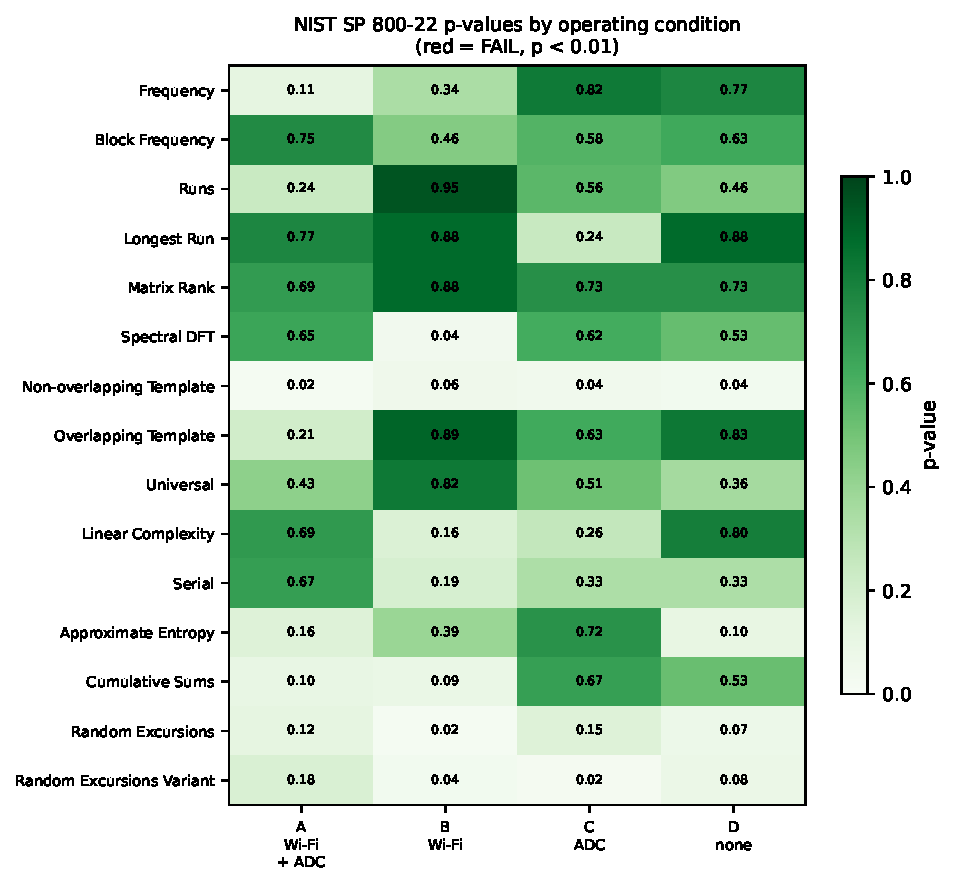
\includegraphics[width=0.8\textwidth]{esp32_nist_heatmap.pdf}
\caption{Valores $p$ de SP~800-22 de las cuatro secuencias de la primera
campaña, uno por condición y prueba, de $10^6$ bits cada una \meas{}. Una
prueba falla por debajo de 0,01; ninguna lo hace. Las pruebas con varios
valores $p$ muestran su mínimo.}
\label{fig:esp32_nist}
\end{figure}

% results/esp32_rng_agosto/nist_summary.csv (15 de 15 en A, B, C, D) y
% nist_results.csv (60 valores p, mínimo 0.0170)
Sobre las cuatro secuencias de la primera campaña la batería pasa las
quince pruebas en las cuatro condiciones (Figura~\ref{fig:esp32_nist}).
La longitud limita lo que eso puede significar. Una fuente perfecta falla
al menos una de quince pruebas con probabilidad
$1-0{,}99^{15} \approx 0{,}14$ (calculado), así que solo un fallo que se
reprodujera indicaría un defecto, y con una secuencia por condición el
análisis de segundo nivel de la norma --- la proporción de secuencias que
pasan y la uniformidad de sus valores $p$ --- no es posible. El menor de
los sesenta valores $p$, 0,017, corresponde a la prueba de plantillas en
la condición~A, y es esperable: el mínimo de $k$ valores $p$ uniformes
tiene una mediana de $1-2^{-1/k}$, que es 0,083 para ocho plantillas y
0,038 para los dieciocho estados de la variante de excursiones
(calculado), y la fila de plantillas (0,017 a 0,055) y la de la variante
(0,020 a 0,176) se sitúan en torno a esas medianas. Nada separa las
condiciones.

Pasar la batería dice que quince estadísticos fijos no distinguen estos
$10^6$ bits de bits independientes y sin sesgo al nivel del 1\,\%. No dice que sean
impredecibles: un generador determinista con una buena función de salida
pasa por diseño, y por eso el NIST decidió en 2022 revisar SP~800-22 y
rechazó su uso para evaluar generadores
criptográficos~\cite{nist_2022_decision}. La condición~D es justo ese caso.
La batería la pasa, Espressif la llama pseudoaleatoria, y la prueba de
reinicios de la Sección~\ref{sec:esp32_90b} muestra que sin el ruido de
arranque es una secuencia fija. La batería sirve aquí como control de
defectos groseros --- sesgo, periodicidad, correlación de corto alcance
--- y no encuentra ninguno.

\section{Entropía de Shannon, tasa y temperatura}
\label{sec:esp32_shannon}

Sobre las mismas cuatro secuencias se calcularon seis métricas más
(\path{analysis/esp32_rng/entropy_analysis.py}). La
Tabla~\ref{tab:esp32_entropy} las da junto al valor que devuelve una
fuente perfecta con la misma longitud, que es la referencia, en lugar del
ideal de una secuencia infinita.

% results/esp32_rng_agosto/entropy_summary.csv; la última fila es calculada
\begin{table}[htbp]
\centering
\caption{Métricas estadísticas de la primera campaña, una secuencia de
$10^6$ bits por condición \meas{}: entropía de Shannon por byte y por bit,
mayor autocorrelación $|r_k|$ para retardos $k$ de 1 a 1000, planitud
espectral de un periodograma de los primeros 65\,536 bits, razón de
compresión de zlib y $\chi^2$ de bytes. La última fila es lo que devuelve
una fuente perfecta con esta longitud (calculado, véase el texto).}
\label{tab:esp32_entropy}
\footnotesize
\begin{tabular}{@{}lllllll@{}}
\toprule
Condición & $H$ (bit/byte) & $H$ (bit/bit) & $\max|r_k|$ & Planitud & zlib & $p$ de $\chi^2$ \\
\midrule
A & 7,99852 & 0,9999982 & 0,00375 & 0,564 & 1,00037 & 0,473 \\
B & 7,99852 & 0,9999993 & 0,00345 & 0,564 & 1,00037 & 0,470 \\
C & 7,99877 & 1,0000000 & 0,00332 & 0,563 & 1,00037 & 0,972 \\
D & 7,99836 & 0,9999999 & 0,00314 & 0,561 & 1,00037 & 0,109 \\
\midrule
Fuente perfecta & $7{,}99853 \pm 0{,}00013$ & $1 - 7\times10^{-7}$ & 0,0034 & 0,561 & $>1$ & uniforme \\
\bottomrule
\end{tabular}
\end{table}

Cada métrica tiene un suelo propio con $10^6$ bits, y la lectura empieza
ahí. La entropía empírica (plug-in) de 125\,000 bytes sobre 256 valores
se queda por debajo de 8~bits incluso para una fuente perfecta, en
$\chi^2_{255}/(2N\ln 2)$, es decir, $0{,}00147 \pm 0{,}00013$~bit; los
cuatro déficits medidos, de 0,0012 a 0,0016~bit, son ese sesgo, y la
entropía de bytes y el $\chi^2$ de bytes son el mismo estadístico en dos
unidades. La entropía por bit reformula la prueba monobit. La
autocorrelación en cada retardo tiene una desviación típica de
$1/\sqrt{n} = 0{,}001$, y el mayor de mil valores así tiene una mediana de
0,0034 para ruido blanco. La planitud de un único periodograma sin
promediar de ruido blanco no es 1 sino $e^{-\gamma} \approx 0{,}561$,
siendo $\gamma$ la constante de Euler, porque cada intervalo de
frecuencia sigue una distribución exponencial. En todas las columnas las
cuatro condiciones quedan donde quedaría una fuente perfecta. Como
SP~800-22, son promedios sobre la salida que una secuencia determinista
puede alcanzar, y la entropía de Shannon no es la magnitud que necesita
una clave: la generación de claves cuenta la min-entropía, el logaritmo
negativo de la probabilidad del resultado más probable, que nunca es
mayor y es el objeto de la Sección~\ref{sec:esp32_90b}.

% throughput_Bps en los tres capture_log.csv: sin la tarea del ADC
% 5214513 a 5218249; con ella 2766632 a 2771781 (primera y segunda
% campañas) y 2703184 a 2705416 (tercera). 64 KiB tardan 12568 us (D)
% y 12559 us (B).
El firmware cronometra la tasa con el temporizador del sistema de
1~$\mu$s sobre 64~KiB, unos 12,6~ms, así que su resolución es mejor que el
0,01\,\% (calculado). En las tres campañas, las doce secuencias sin la
tarea del ADC se generaron a entre 5,21 y 5,22~MB/s ($10^6$~bytes por
segundo), y las doce con ella a 2,77~MB/s en las dos primeras campañas y a
2,70~MB/s en la tercera; la radio cambia la tasa en menos del 0,1\,\%. La
tarea del ADC reduce la tasa a la mitad, por una causa que no se aisló.
Frente al manual, 1,30~millones de palabras por segundo sin la tarea está
por debajo de los 5~MHz del camino de la radio, y de 0,68 a 0,69~millones
con ella está por encima de los 500~kHz del camino SAR: las condiciones A
y C leen de 21,6 a 22,2~Mbit/s mientras que el camino SAR inyecta como
mucho 16~Mbit/s, así que aunque las conversiones de la condición~C
llegaran al generador y cada bit inyectado fuera completamente aleatorio,
detrás de cada bit de salida no podría haber más de 0,72 a 0,74~bit de
ruido nuevo (calculado). El camino de la radio, a 160~Mbit/s, supera casi
cuatro veces la mayor tasa de lectura, 41,7~Mbit/s.

% firmware/esp32_rng/main/temp_monitor.c convierte (F - 32)/1.8 a partir de
% un uint8_t de la ROM; results/esp32_rng_agosto/capture_log.csv solo tiene
% 52.2 y 52.8 (126 y 127 F); temperature_correlation.csv: r = 0.7949,
% p = 0.205; campañas posteriores: los dos capture_log.csv citados arriba.
La temperatura va al final porque su instrumento es el más tosco. El
firmware lee el sensor mediante una función de la ROM no documentada que
devuelve un entero de 8 bits sin calibrar en grados Fahrenheit, así que un
paso es $5/9$~$^\circ$C, 0,556~$^\circ$C. En la primera campaña solo
devolvió 52,2 y 52,8~$^\circ$C, que son 126 y 127~$^\circ$F: todo el rango
de temperatura de la campaña es un paso del sensor. La correlación entre
la entropía de bytes y la temperatura sobre las cuatro secuencias,
$r = 0{,}795$ con $p = 0{,}21$, se calculó por tanto frente al bit menos
significativo del sensor, y no aporta información; no se afirma ningún
efecto de la temperatura, en ningún sentido. Los dos chips identificados
leyeron después de 49,4 a 51,7 y de 61,7 a 64,4~$^\circ$C en la misma
escala sin calibrar, así que chip y temperatura están confundidos. Un
estudio de temperatura necesita un sensor calibrado y un barrido
controlado, y no se hizo ninguno.

\section{Un recolector de claves multifuente}
\label{sec:esp32_harvester}

% firmware/esp32_rng/main/entropy_harvester.c, adc_noise.c, sram_puf.c
Si no se puede confiar en el generador con la radio apagada, un nodo que
mantiene la radio apagada necesita otras fuentes. Esta parte del trabajo
construyó un recolector (\path{firmware/esp32_rng/main/entropy_harvester.c})
que añade dos fuentes del mismo chip cuya disponibilidad complementa la
del generador: el patrón de arranque de la SRAM, presente en cada
encendido antes de que arranque ningún periférico~\cite{holcomb_2009_powerup},
y los bits menos significativos del ADC leyendo una entrada flotante.
Estas pasan por la corrección de Von
Neumann~\cite{vonneumann_1951_various}, que descarta los pares 00 y 11 y
convierte 01 en 0 y 10 en 1, de modo que bits independientes salen sin
sesgo a costa de al menos tres cuartas partes de ellos. Las aportaciones
se acondicionan con SHA-256 en una reserva (\emph{pool}) de 256 bits,
\begin{equation}
\mathrm{pool}_0 = \mathrm{SHA256}\bigl(r \,\|\, \mathrm{SHA256}(S) \,\|\,
a \,\|\, \texttt{"TFM0"}\bigr),
\label{eq:esp32_pool}
\end{equation}
donde $r$ son 32 bytes de \texttt{esp\_fill\_random()}, $S$ el patrón de
SRAM de 4~KiB, $a$ 32 bytes de bits del ADC corregidos y el último campo
una etiqueta que separa este uso del hash de los demás. Cada salida de
32 bytes aplica el hash a la reserva junto con un contador y una lectura
nueva del generador, y después la reserva avanza como un trinquete
(ratchet),
\begin{equation}
o_i = \mathrm{SHA256}(\mathrm{pool} \,\|\, i \,\|\, r_i), \qquad
\mathrm{pool} \leftarrow \mathrm{SHA256}(\mathrm{pool} \,\|\, o_i),
\label{eq:esp32_ratchet}
\end{equation}
de modo que una reserva capturada tras la salida $i$ no permite obtener
las anteriores; un resembrado incorpora a la reserva, mediante el hash,
datos nuevos del generador y del ADC. Concatenar antes de aplicar el hash
da la única garantía que no necesita independencia entre fuentes que
comparten chip, alimentación y temperatura:
$H_\infty(X_1 \| X_2 \| X_3) \geq \max_i H_\infty(X_i)$.

% analysis/esp32_rng/harvester_from_sources.py: entradas puf_boot1.bin y
% condD_rep1.bin, campo del ADC = 32 B del mismo flujo del RNG (sustituto).
% docs/esp32_linea_base_90b.md 1 y 5: el firmware recompilado se detiene en
% la generación de semillas tras el primer ciclo.
% results/esp32_rng_agosto/harvester_validation.csv: 1000 de 1000 únicas,
% chi2 de bytes p = 0.300811, Hamming 128.050 +- 8.027 bits, 7 valores p
% de NIST de 0.147738 a 0.955784.
El recolector se validó fuera de línea. Las semillas producidas en el
dispositivo no se capturaron de forma fiable en la primera campaña, y el
firmware recompilado después se detiene durante la generación de
semillas, un fallo que no se investigó porque las semillas no intervienen
en las demás medidas. La validación reproduce por tanto la construcción
en Python (\path{analysis/esp32_rng/harvester_from_sources.py}) sobre
datos capturados: un patrón de SRAM; la secuencia de la condición~D como
aportación del generador, la peor condición, a propósito; y 32 bytes de
la misma secuencia en lugar del campo del ADC, del que no existe una
captura aparte. De las 1000 semillas de 32 bytes así derivadas, todas son
distintas y sus bytes son uniformes ($\chi^2$ $p = 0{,}30$); la distancia
de Hamming entre dos semillas, sobre 20\,000 pares aleatorios, promedia
128,05 de 256 bits (50,02\,\%) con una desviación típica de 8,03, frente a
128 y 8 para semillas uniformes independientes; y las siete pruebas de
SP~800-22 aplicables a los 256\,000 bits del flujo de semillas pasan, con
$p$ de 0,148 a 0,956.

% calculado a partir de results/esp32_rng_agosto/puf_pc1-4.bin (serie limpia:
% pesos 49.61 a 49.74 %, pares 6.45 a 6.81 %, media 6.63 %, estables
% 28804 de 32768 = 87.90 %) y puf_boot1-5.bin (serie mixta: pesos
% 49.63 a 49.86 %, boot1 frente al resto 49.55 a 49.74 %, pares entre
% boot2-5 6.48 a 7.43 %, estables en boot2-5 28719 de 32768 = 87.64 %,
% la cifra de docs/plan.md 9); 23.9 % en harvester_validation.csv.
La fuente SRAM se caracterizó por separado. Solo un corte de alimentación
vuelve a aleatorizar las celdas, ya que un reinicio que mantiene la
alimentación deja en el búfer lo que escribiera la ejecución anterior, así
que se capturó una serie limpia de cuatro patrones con un ciclo de
alimentación antes de cada uno. Los nueve patrones capturados tienen un
peso de Hamming del 49,6 al 49,9\,\%, y las seis distancias de la serie
limpia van del 6,45 al 6,81\,\%, con una media del 6,63\,\%. La fracción de
celdas estables, las que leen el mismo valor en los cuatro encendidos, se
midió directamente: 87,90\,\% en la serie limpia y 87,64\,\% en los cuatro
encendidos de la primera serie, la mixta, así que unas 4000 de las
32\,768 celdas cambiaron al menos una vez. El primer análisis había
inferido un 93\,\% aproximadamente a partir de la distancia media, que
cuenta con qué frecuencia difieren dos encendidos, no cuántas celdas
difieren alguna vez; la cifra que se usa es la contada
(Sección~\ref{sec:conventions}). La distancia entre arranques del
23,9\,\% calculada inicialmente para la fuente no es una cifra limpia:
promedia diez pares de una serie que mezclaba ciclos de alimentación con
reinicios que mantenían la alimentación, en la que un patrón difiere de
los otros cuatro en el 49,6 al 49,7\,\% de sus bits, como lo harían datos
no relacionados, y los otros seis pares difieren en el 6,5 al 7,4\,\%,
como lo hacen los encendidos de las mismas celdas.

% analysis/esp32_rng/mqtt_tls_demo.py, modo fuera de línea; resultado según
% las notas de la primera campaña (sesión segura).
La validación muestra que la construcción se implementó tal como se
diseñó, no que las semillas lleven entropía. Todas las comprobaciones se
pasan por construcción: el contador hace que cada salida sea distinta
aunque todas las demás entradas fueran constantes, y SHA-256 convierte
entradas distintas cualesquiera en salidas que parecen uniformes y distan
media palabra entre sí. Las entradas de esta validación lo ilustran. El
campo de SRAM fue un mismo patrón para las 1000 semillas --- el primero
de la serie mixta, que no es un estado de encendido --- y la única
entrada que cambiaba entre semillas era la salida de la condición~D, que
la prueba de reinicios muestra que es una secuencia fija una vez
eliminado el ruido de arranque. La entropía de una semilla es como mucho
$\min(256, H_\infty)$ bits, siendo $H_\infty$ la min-entropía de las
entradas, y esta no se midió para ninguna de ellas. Un peso del 50\,\% no
cambia esto: el 88\,\% de las celdas de la SRAM son una huella fija,
conocida por cualquiera que haya leído el patrón una vez, y acotar lo que
aporta el 12\,\% restante requeriría muchos más encendidos y un modelo de
las celdas. El recolector es una arquitectura cuya salida es al menos tan
fuerte como su mejor fuente, no una fuente de entropía medida. Una
demostración fuera de línea de su uso previsto
(\path{analysis/esp32_rng/mqtt_tls_demo.py}) expande una semilla en una
clave de sesión con HKDF-SHA256~\cite{krawczyk_2010_hkdf} y protege un
mensaje con AES-256-GCM, rechazando un mensaje reenviado y otro
manipulado; ejercita la criptografía, y la clave hereda la entropía de la
semilla sin añadir ninguna.

\section{La referencia del ESP32 frente a SP 800-90B}
\label{sec:esp32_90b}

O8 pide una comparación numérica con el ESP32, y la mitad puede cerrarse
sin la placa: el lado de la referencia. Las
Secciones~\ref{sec:esp32_sp80022} y~\ref{sec:esp32_shannon} aplicaron
SP~800-22 y la entropía de Shannon a la primera campaña; los estimadores
de SP 800-90B se aplican aquí a las tres, que en conjunto dan seis
repeticiones de $10^6$ bits por condición, tres en cada uno de los dos
chips del mismo modelo (ESP32-D0WD-V3). Otras dos capturas con la radio
apagada, de $3{,}52\times10^6$ y $8{,}38\times10^6$ bits, se tomaron con
el firmware verificador del Capítulo~\ref{ch:ch5_verification}. Las
veintiséis se pasaron por la implementación de referencia del \ac{NIST} de
los estimadores de SP 800-90B~\cite{nist_ea_github, turan_2018_sp80090b}
(versión 1.1.8), por la vía IID y por la vía no IID, en el formato
binario que la norma prescribe para fuentes de bits. La
Tabla~\ref{tab:esp32_90b} recoge el resultado.

\begin{table}[htbp]
\centering
\caption{El generador del ESP32 frente a los estimadores de SP 800-90B \meas{}.
Condiciones A--D: seis repeticiones de $10^6$ bits cada una, tres en cada
uno de los dos chips, media y rango sobre las repeticiones; E y F:
capturas únicas de $3{,}5\times10^6$ y $8{,}4\times10^6$ bits. El techo es
el valor más alto que el estimador del valor más común (MCV) puede
devolver para una fuente perfectamente uniforme de esa longitud con un
99\,\% de confianza; la cifra no IID es el mínimo de los diez estimadores
de la Sección~6.3 de la norma, y la última columna nombra el estimador que
la fijó (veces de seis). Los veredictos de la vía IID se discuten en el
texto.}
\label{tab:esp32_90b}
\footnotesize
\begin{tabular}{@{}llrrll@{}}
\toprule
Captura & Condición & $H$ (IID) & Techo & $H$ (no IID) & Limitante \\
\midrule
A & Wi-Fi + ADC & 0,9954 & 0,9963 & 0,844 (0,812--0,877) & Compresión 5, Lag 1 \\
B & Wi-Fi       & 0,9951 & 0,9963 & 0,862 (0,824--0,898) & Compresión 5, LRS 1 \\
C & ADC         & 0,9952 & 0,9963 & 0,836 (0,812--0,867) & Compresión 6 \\
D & ninguna     & 0,9957 & 0,9963 & 0,857 (0,832--0,916) & Compresión 5, Colisión 1 \\
E (verificador) & ninguna & 0,9977 & 0,9980 & 0,867 & Compresión \\
F (verificador) & ninguna & 0,9982 & 0,9987 & 0,911 & Compresión \\
\bottomrule
\end{tabular}
\end{table}

La resolución va primero, como en todo este trabajo. El estimador MCV
devuelve $-\log_2 p_u$ con $p_u = \hat p + 2{,}576\sqrt{\hat p(1-\hat p)/N}$,
de modo que ni siquiera una fuente perfecta puede puntuar por encima de
0,9963 con $10^6$ bits, de 0,9980 con $3{,}5\times10^6$ ni de 0,9987 con
$8{,}4\times10^6$. Cada una de las veintiséis capturas queda a menos de
0,0035 de ese techo, y ninguna implica un sesgo de unos superior a
$2{,}4\sigma$, que es lo que se observa en veintiséis extracciones de una
fuente sin sesgo.

La vía IID necesita una calibración antes de que puedan leerse sus
veredictos. De las cincuenta y dos ejecuciones (veintiséis capturas en los
formatos de bits y de bytes), cuatro fallan una sola prueba, nunca el
mismo fichero en ambos formatos: una prueba de permutación en cada formato
y dos pruebas $\chi^2$ en el formato de bytes. La frecuencia con que datos
buenos fallan estas pruebas a esa misma longitud no es el $10^{-3}$
nominal, así que se midió, ejecutando la misma herramienta sobre 1000
ficheros de 125\,000 bytes y 200 ficheros de $10^6$ bits del generador del
sistema operativo. En el formato de bytes, la batería de permutación falla
en el 1,9\,\% de los ficheros buenos y el par $\chi^2$ en el 2,4\,\%; en el
formato de bits, la batería de permutación falla en el 2,5\,\% y el par
$\chi^2$ en ninguno de los 200. La cifra de $\chi^2$ se rastreó hasta su
causa reimplementando ambas pruebas, lo que reproduce los cincuenta y dos
valores $p$ de la herramienta hasta la sexta cifra decimal, y ejecutándolas
sobre 5000 ficheros buenos. La prueba de independencia del formato de
bytes reparte 62\,500 pares sin solape entre 65\,536 celdas y agrupa celdas
hasta que cada grupo espera cinco cuentas, pero a esta longitud su $p$ no
es uniforme: la mediana es 0,175 en lugar de 0,5, y cae por debajo de
$10^{-3}$ en el 1,7\,\% de los ficheros, diecisiete veces la tasa nominal.
Las otras tres pruebas $\chi^2$ están bien calibradas, y el defecto
desaparece a partir de $10^6$ bytes. Frente a estas tasas, los fallos del
ESP32 no tienen nada de particular: un fallo de permutación en veintiséis
ejecuciones en formato de bytes donde se esperan 0,49 ($P = 0{,}39$), dos
fallos $\chi^2$ donde se esperan 0,62 ($P = 0{,}13$), y un fallo de
permutación en el formato de bits donde se esperan 0,65 ($P = 0{,}48$). En
un chip, la prueba de independencia de bytes dio $p < 0{,}05$ en seis
capturas de doce, frente a 2,9 esperadas; agrupar las capturas de cada
chip, donde la prueba está calibrada y es más potente, da valores $p$
empíricos de 0,82 y 0,96 en ese chip para pares de bytes alineados con la
palabra de 32 bits y desplazados un byte, y de 0,38 y 0,86 en el otro, así
que no hay dependencia entre bytes vecinos. El suceso más raro es el fallo
de bondad de ajuste de la primera captura de la condición~D
($p = 2{,}4\times10^{-4}$): esa prueba falla en el 0,04\,\% de los ficheros
buenos, así que un fallo así en veintiséis tiene una probabilidad cercana
al 1\,\%. No se reprodujo en las cinco capturas posteriores de la misma
condición ($p = 0{,}32$ a $0{,}96$) ni en E y F, y se registra como azar;
la advertencia de Espressif de que la aleatoriedad del generador no está
garantizada sin la radio o el ADC sigue en pie como una advertencia que
estas pruebas no ven. Formalmente, un único fallo retira la hipótesis IID
para esa captura; como la cifra que se retiene es la no IID, nada de lo
que sigue depende de ello. Leída con su calibración, la vía IID encuentra
la salida del ESP32 indistinguible de una fuente binaria de entropía
completa con este tamaño de muestra. Es el mismo veredicto que dio
SP 800-22, alcanzado por otro camino, y dice lo mismo: no se ve nada mal.

La vía no IID dice otra cosa, y leerla bien importa más que el número. En
veinticinco de las veintiséis capturas, su mínimo lo fija uno de tres
estimadores --- compresión, colisión o subcadena repetida más larga --- con
0,81 a 0,92 bit por bit; en la restante, el predictor Lag, con 0,88; los
estimadores MCV y de Markov nunca bajan de 0,99. Se sabe que esos tres
estimadores son conservadores con datos casi uniformes~\cite{zhu_2017_analysis};
los predictores de Kelsey, McKay y S\"onmez Turan~\cite{kelsey_2015_predictive}
se introdujeron precisamente porque los estimadores anteriores de la norma
juzgan mal fuentes de ese tipo. Las repeticiones muestran que esto es un
comportamiento de los estimadores y no una propiedad de las condiciones.
La estimación por compresión tiene una desviación típica de 0,02 a 0,04
\emph{dentro} de una condición, tan grande como el 0,03 que separa las
medias de las cuatro condiciones, y un análisis de la varianza de un factor
sobre cada uno de los once estimadores no encuentra diferencia entre
condiciones: el $p$ más pequeño es 0,083, para el predictor MultiMCW, por
encima del 0,05 sin corregir y muy por encima del 0,0045 que exigen once
pruebas. Lo mismo vale entre chips. Agrupando las condiciones, que no
difieren, ningún estimador separa las doce capturas de cada chip al nivel
corregido; el $p$ más pequeño, 0,047 para MCV, corresponde a una
diferencia de 0,0007 bit por bit junto al techo de resolución, y un valor
por debajo de 0,05 entre once pruebas es lo que da el azar. El mínimo no
IID es 0,852 en un chip y 0,847 en el otro: con dos dispositivos, la
referencia no depende de cuál se mida, a la resolución de estos
estimadores. La captura más grande añade una segunda muestra del efecto
de la resolución: en el formato de bytes, su estimador limitante es la
prueba de $t$-tupla con $t = 2$, que devuelve 7,39 bits por byte porque
$10^6$ bytes contienen demasiado pocos de los 65\,536 pares posibles para
que el más frecuente sea representativo, exactamente como le ocurre al
techo del MCV con $t = 1$. Ningún estimador resuelve con seis
repeticiones diferencia alguna entre Wi-Fi encendido, ADC encendido y
ninguno de los dos, y no se afirma ninguna.

La prueba de reinicios de la Sección~3.1.4 de la norma responde a lo que
la estadística anterior no puede: si un generador no tiene ruido propio,
su salida tras un reinicio en frío debe repetirse. Un firmware dedicado
leyó 1024~bytes con \texttt{esp\_fill\_random} como primera acción de la
aplicación, con la radio y el ADC apagados (condición~D), y el chip de MAC
a0:dd:6c:0e:fb:4c se reinició 1000 veces por su patilla de habilitación;
la ROM de arranque notificó un reinicio por encendido todas las veces. Dos
variantes comparten la aplicación y difieren solo en el bootloader de
segunda etapa: el de serie, que inyecta ruido del SAR ADC en el generador
durante unos 126~ms mientras se ejecuta, y el mismo bootloader con esa
llamada desviada a una función vacía en tiempo de enlazado, lo que
confirma el desensamblado. Otras tres variantes hacen una segunda lectura
tras arrancar el Wi-Fi como en las condiciones A y B, sin asociarse a
ninguna red, y esperar 200~ms, con cada uno de los dos bootloaders; la
tercera es un control que espera el mismo tiempo sin tocar la radio, de
modo que la lectura cae en el mismo tick del planificador. La
Tabla~\ref{tab:esp32_restart} recoge el resultado.

\begin{table}[htbp]
\centering
\caption{Prueba de reinicios del generador del ESP32 \meas{}: 1000 reinicios
en frío por variante, un chip. $H_r$ y $H_c$ son el mínimo de los
estimadores no IID sobre el conjunto de filas y el conjunto de columnas de
la norma (1000 reinicios $\times$ 1000 bits); la prueba falla cuando
cualquiera de los dos queda por debajo de la mitad de la estimación
inicial $H_I$, la cifra no IID más baja de este chip en la misma condición
(0,838 bit por bit en D, 0,859 en B). El formato de bytes da los mismos
veredictos. Los solapes son reinicios cuya salida aparece desplazada
dentro de la de otro, todos idénticos palabra por palabra. Las lecturas
tardías caen entre 352 y 412~ms después de que arranque la aplicación, la
mayoría a 352~ms.}
\label{tab:esp32_restart}
\footnotesize
\begin{tabular}{@{}llrrrl@{}}
\toprule
Bootloader & Lectura & $H_r$ / $H_c$ & Distintas & Solapes & Veredicto \\
\midrule
De serie & en el arranque, radio apagada & 0,898 / 0,854 & 1000 & 0 & pasa \\
Sin ruido de arranque & en el arranque, radio apagada & 0,024 / 0,813 & 759 & 5424 & falla \\
Sin ruido de arranque & tardía, radio apagada (control) & 0,024 / 0,808 & 760 & 5632 & falla \\
Sin ruido de arranque & tardía, Wi-Fi encendido & 0,831 / 0,845 & 1000 & 0 & pasa \\
De serie & tardía, Wi-Fi encendido & 0,844 / 0,807 & 1000 & 0 & pasa \\
\bottomrule
\end{tabular}
\end{table}

Con el bootloader de serie el generador pasa en ambos formatos, y las
1000 salidas difieren entre sí exactamente como lo harían datos
aleatorios: la distancia de Hamming media entre dos reinicios es de 4096,0
bits de 8192, frente a $4096 \pm 45$ esperados. Sin el ruido de arranque
falla de forma tajante, y los datos muestran por qué. Cada reinicio es una
ventana sobre una única secuencia fija, leída desde un punto de partida
ligeramente distinto: dondequiera que el comienzo de la salida de un
reinicio aparece dentro de la de otro, desplazado unas pocas palabras de
32 bits, todo el solape coincide palabra por palabra, 5424 veces sin una
sola diferencia. Lo único que cambia entre reinicios es el instante en que
la aplicación empieza a leer, que varía en unos pocos miles de ciclos de
reloj de un arranque al siguiente. Eso vale entre 6,5 bits por reinicio,
la cota de la norma a partir de la salida más repetida, y 10,8 bits si
todos los puntos de partida fueran igual de probables, de 8192 bits leídos.
Con la radio y el ADC apagados el generador no tiene ruido propio, y la
afirmación de Espressif de que entonces su salida es solo
pseudoaleatoria~\cite{espressif_idf_random} queda confirmada directamente,
cosa que ninguna prueba estadística sobre un flujo continuo podría hacer.
De ello se siguen dos consecuencias. Las capturas de la condición~D de la
Tabla~\ref{tab:esp32_90b} son la salida de un generador determinista
sembrado durante el arranque: los estimadores les acreditan 0,85 bit por
bit, tanto como con la radio encendida, mientras que su entropía física es
como mucho la que inyectó el bootloader, que esos estimadores no miden. Y
una aplicación que deriva una clave justo después del arranque con la
radio apagada depende por completo del ruido del bootloader de serie; sin
él, la clave podría adivinarse en unos pocos miles de intentos, el
problema del arranque en frío descrito por Blanco-Romero
et al.~\cite{blancoromero_2026_entropy}.

Las filas con radio responden a la otra mitad de la afirmación de
Espressif. Sin el ruido de arranque, arrancar el Wi-Fi basta para que la
prueba pase: las 1000 salidas son todas distintas, no se comparte ninguna
ventana, y los 289 pares de reinicios que leían valores idénticos antes de
arrancar la radio leen 289 valores diferentes después. La temporización
por sí sola no lo explica. El control espera el mismo tiempo y lee en el
mismo tick del planificador, con un instante de lectura que varía otro
tanto (3824 frente a 5260 ciclos de reloj entre los reinicios que
comparten el tick), y se repite exactamente como en el arranque: 760
salidas distintas, 5632 solapes idénticos, unos 1700 estados. Con tan
pocos estados, los 797 reinicios que comparten un tick en la variante con
radio mostrarían unas 180 repeticiones solo por temporización; no muestran
ninguna. Sin la radio, el generador no recibe ruido en sus primeros
350~ms de funcionamiento; con la radio, sí. Lo que la prueba no da es
cuánta entropía por bit aporta la radio: los 0,83 bit por bit validados
son la cifra de los estimadores, con su sesgo habitual, no una medida del
ruido de la radio. No se ha encontrado en la bibliografía consultada una
prueba de reinicios del generador del ESP32.

\section{Lo que una caja negra puede decir y lo que no}
\label{sec:esp32_lessons}

Todos los instrumentos estadísticos aplicados al generador del ESP32 dan
la misma respuesta. SP~800-22 pasa las quince pruebas en las cuatro
condiciones; las métricas de Shannon, de autocorrelación, espectrales y de
compresión quedan donde quedaría una fuente perfecta con esta longitud;
la vía IID de SP~800-90B, leída con su calibración, encuentra la salida
indistinguible de una fuente binaria de entropía completa; y la vía no
IID acredita de 0,81 a 0,92~bit por bit, sin ninguna diferencia entre
condiciones o entre chips que resuelva algún estimador. Ninguna de estas
cifras distingue la condición~D, en la que Espressif dice que el
generador es pseudoaleatorio, de la condición~A, en la que están activas
las dos fuentes documentadas.

La prueba de reinicios es la única medida que lo hace, porque plantea una
pregunta física y no estadística: ¿se repite la salida cuando el
generador vuelve a arrancar desde el mismo estado? Sin el ruido de
arranque y con la radio apagada se repite, palabra por palabra; con la
radio encendida, no. El generador no tiene ruido propio con la radio y el
ADC apagados, y la radio sí le inyecta ruido. Las cifras de SP~800-90B de
la condición~D son, por tanto, el veredicto de los estimadores sobre la
continuación determinista de una semilla de arranque: una cifra
estadística, que no puede acreditarse como entropía física. Lo mismo
vale, de forma menos visible, para las demás condiciones. La prueba de
reinicios muestra que la radio inyecta ruido, no cuánto; para las
condiciones A y C ni siquiera está establecido que las conversiones del
ADC lleguen al generador, y según las propias tasas del manual el camino
SAR no podría aportar un bit de ruido nuevo por bit de salida a la tasa a
la que se leyó el generador.

Lo que falta no es una prueba mejor sino un tipo distinto de
conocimiento: un modelo de la fuente --- qué proceso físico produce la
aleatoriedad, y con qué parámetros --- y una medida de esos parámetros que
acote la min-entropía por debajo. Ninguna de las dos cosas puede
obtenerse desde fuera del ESP32: sus fuentes de ruido, su estado interno
y su posprocesado no están documentados, y los estimadores de
SP~800-90B se diseñaron para muestras de ruido en bruto, no para la
salida de un bloque que puede estar ya acondicionado. Por eso la segunda
parte de este trabajo construye el generador en lugar de medir el de
otro. El Capítulo~\ref{ch:ch3_entropy} parte de la física de un oscilador
en anillo, extrae su jitter y lo convierte, mediante un modelo validado,
en una cota inferior de la min-entropía; los capítulos siguientes
construyen y verifican el motor en torno a esa fuente. El ESP32 sigue en
el trabajo con otros dos papeles: su cifra no IID es la referencia de la
comparación de la Sección~\ref{sec:esp32_ref}, y su biblioteca
criptográfica es la implementación independiente con la que se verifica
el motor.

\chapter{Fuente de entropía: del transistor a la min-entropía}
\label{ch:ch3_entropy}

% [BORRADOR v1 -- solo teoría y simulación; cifras de hardware pendientes]
% Material de partida: docs/modelo_ero_resultados.md, docs/arquitectura.md,
% analysis/ero_model.py, analysis/jitter_estimator.py, analysis/spice_ring.py

Este capítulo construye la cadena sobre la que descansa el resto del TFM:
del jitter físico de un oscilador en anillo a una cifra defendible de
min-entropía por bit de salida, y de esa cifra a los parámetros de diseño
del muestreador. Cada paso se valida antes de usarse. Los estimadores
estadísticos se validan con datos sintéticos de jitter conocido; las cotas
analíticas se validan frente a un cálculo numérico exacto; y el banco a
nivel de transistor se valida midiendo su propia resolución antes de medir
nada con él. Todas las cifras de este capítulo son \simu{} salvo que se
indique lo contrario; la campaña de hardware se presenta en el
Capítulo~\ref{ch:ch7_results}.

\section{El oscilador en anillo elemental}
\label{sec:ero}

La fuente de entropía es un \ac{ERO}: un oscilador en anillo libre RO1
cuya salida se muestrea con un flip-flop que recibe como reloj un segundo
oscilador en anillo RO2 dividido por un entero $K_D$~\cite{baudet_2011_security,
fischer_2014_embedded}. Entre dos muestras, la fase de RO1 acumula jitter
durante $K_D$ periodos de RO2; cuando el jitter acumulado es comparable al
periodo de RO1, el bit muestreado se vuelve impredecible. Se eligió el
\ac{ERO} frente a alternativas de mayor tasa de bits (XOR de varios
anillos, muestreo coherente, anillos de efecto de transición) por una sola
razón: es la arquitectura para la que existe un modelo estocástico con una
cota de entropía demostrable y para la que se ha publicado y validado un
método embebido de medida del jitter~\cite{petura_2016_survey}. La tasa de
bits no es un requisito aquí ---el motor solo consume entropía para dar
semilla a un generador determinista---, mientras que una cota demostrable
sí lo es.

Una decisión de diseño que se deriva de la plataforma es que \emph{el
oscilador de la placa nunca se usa como referencia}. La fuente de reloj de
la Basys~3 es un oscilador MEMS con un \ac{PLL} fraccional cuya hoja de
características especifica un jitter ciclo a ciclo de hasta 95~ps
\est{}~\cite{digilent_2014_basys3rm}, entre uno y dos órdenes de magnitud
por encima del jitter por periodo de un oscilador en anillo en un proceso
de 28~nm (2--4~ps \est{}~\cite{petura_2016_survey}). Muestrear RO1 con ese
reloj mediría el ruido de fase del PLL, una componente global y
potencialmente inducible, en lugar del ruido térmico del anillo. Por eso
RO2 muestrea a RO1, y el reloj de sistema de 100~MHz solo gobierna la
lógica síncrona.

\section{Modelo estocástico y factor de calidad}
\label{sec:model}

Siguiendo a Baudet \emph{et al.}~\cite{baudet_2011_security}, la fase
$\varphi(t)$ de RO1, medida en periodos, se modela como un proceso de
Wiener con deriva $\mu$ y volatilidad $\sigma^2$. Entre dos muestras
separadas $\Delta t$, la fase avanza en promedio $\nu = \mu\,\Delta t$
periodos y acumula una varianza
\begin{equation}
  Q = \sigma^2\,\Delta t ,
  \label{eq:Q}
\end{equation}
el \emph{factor de calidad}. El bit de salida es $s = 1$ cuando la fase
fraccionaria está en $[1/2, 1)$. Condicionado a la fase anterior
$\varphi_0$, el bit sigue una distribución de Bernoulli con
\begin{equation}
  P(s=1 \mid \varphi_0) = \sum_{k\in\mathbb{Z}}
  \left[\Phi\!\left(\tfrac{k+1-\varphi_0-\nu}{\sqrt{Q}}\right) -
        \Phi\!\left(\tfrac{k+\tfrac12-\varphi_0-\nu}{\sqrt{Q}}\right)\right],
  \label{eq:puno}
\end{equation}
donde $\Phi$ es la función de distribución normal estándar; se trata de la
gaussiana envuelta evaluada de forma exacta. Su primer armónico da el sesgo
máximo $\varepsilon_{\max} \approx (2/\pi)\,e^{-2\pi^2 Q}$, a partir del
cual el Corolario~1 de Baudet proporciona la conocida expresión
\begin{equation}
  H(s \mid \varphi_0) = 1 - \frac{4}{\pi^2 \ln 2}\, e^{-4\pi^2 Q}
  + O\!\left(e^{-6\pi^2 Q}\right).
  \label{eq:baudet14}
\end{equation}

\section{Entropía condicional exacta frente a la cota asintótica}
\label{sec:exact}

La ecuación~\eqref{eq:baudet14} se cita habitualmente como una \emph{cota
inferior} de la entropía por bit. Leída con atención, la desigualdad del
corolario solo afirma que la tasa de entropía de la secuencia es al menos
la entropía de un bit condicionada a la fase anterior exacta; el miembro
derecho es un desarrollo asintótico \emph{de} esa entropía condicional, no
una cota de ella. Desarrollando la entropía binaria en función del sesgo,
$h_2(\tfrac12+\varepsilon) = 1 - \tfrac{1}{\ln 2}\sum_{n\ge1}
\tfrac{(2\varepsilon)^{2n}}{2n(2n-1)}$, y promediando sobre una $\varphi_0$
uniforme con $\varepsilon = A\sin(2\pi\varphi)$,
$A = (2/\pi)e^{-2\pi^2 Q}$, se obtiene
\begin{equation}
  H(s\mid\varphi_0) = 1 - \frac{4}{\pi^2\ln 2}\,e^{-4\pi^2 Q}
                        - \frac{8}{\pi^4\ln 2}\,e^{-8\pi^2 Q} - \cdots
  \label{eq:orden2}
\end{equation}
Todos los términos omitidos son negativos, así que \emph{cualquier}
truncamiento sobrestima la entropía; el término siguiente decae como
$e^{-8\pi^2 Q}$, no como $e^{-6\pi^2 Q}$. La Tabla~\ref{tab:exact}
compara el valor exacto, calculado a partir de \eqref{eq:puno} sobre una
malla de 8192 fases, con los desarrollos de primer y segundo orden. Añadir
el término de segundo orden reduce el error de \eqref{eq:baudet14} en un
factor de 95 para $Q=0{,}10$ y de 4970 para $Q=0{,}20$, lo que confirma la
deducción.

\begin{table}[htbp]
\centering
\caption{Entropía de Shannon condicional por bit: cálculo exacto con la
gaussiana envuelta frente a desarrollos truncados \simu{}.}
\label{tab:exact}
\begin{tabular}{@{}lcccc@{}}
\toprule
$Q$ & Exacta & Orden 2 & Orden 1 (Ec.~\ref{eq:baudet14}) & Error del orden 1 \\
\midrule
0,02 & 0,7013194 & 0,7100952 & 0,7345213 & $+3{,}3\times10^{-2}$ \\
0,05 & 0,9163001 & 0,9164920 & 0,9187783 & $+2{,}5\times10^{-3}$ \\
0,10 & 0,9886728 & 0,9886733 & 0,9887174 & $+4{,}5\times10^{-5}$ \\
0,15 & 0,9984319 & 0,9984319 & 0,9984327 & $+8{,}5\times10^{-7}$ \\
0,20 & 0,9997823 & 0,9997823 & 0,9997823 & $+1{,}6\times10^{-8}$ \\
\bottomrule
\end{tabular}
\end{table}

En la región de funcionamiento ($Q\approx0{,}2$) la discrepancia es de
$10^{-8}$ e irrelevante; para un generador infradimensionado
($Q\approx0{,}02$) la fórmula truncada atribuye un 3,3\,\% de entropía que
no existe. Por ello, este TFM usa el cálculo exacto como valor conservador
y cita \eqref{eq:baudet14} como lo que es: una aproximación asintótica
excelente para $Q \gtrsim 0{,}1$. La misma herramienta numérica muestra que
la min-entropía obtenida a partir del sesgo del primer armónico,
$H_\infty = -\log_2(\tfrac12 + \varepsilon_{\max})$, coincide con el valor
exacto del peor caso con un error inferior a $10^{-4}$~bit en
$Q\in[0{,}05;\,0{,}30]$.

\subsection{Objetivo de diseño}

La versión~3.0 de AIS~20/31~\cite{peter_2024_ais31} admite dos criterios
alternativos para la clase PTG.2: entropía de Shannon $\ge 0{,}9998$ o
min-entropía $\ge 0{,}98$ por bit interno. Resolver ambos por bisección
sobre las entropías exactas da $Q \ge 0{,}2022$ y $Q \ge 0{,}2286$,
respectivamente. El criterio de min-entropía es el más exigente y es
también la magnitud con la que trabaja NIST SP~800-90B, por lo que es el
que se adopta aquí: \textbf{el objetivo de diseño es $Q \ge 0{,}23$, con
un punto de consigna de $Q = 0{,}30$} ($H_\infty = 0{,}9951$), con un
margen que cubre la reducción del jitter térmico a baja temperatura, que
es la prueba adversaria estándar de Fischer y
Lubicz~\cite{fischer_2014_embedded}.

\section{Estimador embebido del jitter y sus dos correcciones}
\label{sec:estimator}

Para elegir $K_D$ hay que conocer $\sigma^2$, y el método de Fischer y
Lubicz~\cite{fischer_2014_embedded} la mide a partir de los propios bits:
con $K_D = 1$, la fracción $c$ de pares $(b_j, b_{j+M})$ que difieren
dentro de un bloque de $N$ pares estima la fase acumulada a lo largo de
$M$ muestras, y su varianza entre $K$ bloques crece como
$4 M Q_{\mathrm{bruto}}$. Implementado al pie de la letra, con un ajuste a
una recta, el estimador \emph{subestima} $Q_{\mathrm{bruto}}$ entre un
13\,\% y un 38\,\% según el nivel de jitter. Se identificaron dos causas
sobre datos sintéticos con $Q$ conocido, y se corrigieron:

\begin{enumerate}
\item \textbf{Efecto de vértice.} $c$ no es lineal en la fase acumulada;
es una onda \emph{triangular} de periodo uno y pendiente $\pm2$. Cuando la
fase determinista $M\nu \bmod 1$ cae cerca de un vértice, la distribución
queda a ambos lados de él y la varianza se desploma ---hasta 0,38 de su
valor nominal en un caso medido---. El vértice se detecta a partir de la
propia media medida ($\bar c \approx 0$ o $1$ es un vértice;
$\bar c \approx \tfrac12$, el centro de la rampa), de modo que las
distancias $M$ con $\bar c$ fuera de $[0{,}15;\,0{,}85]$, o para las que
$3\sqrt{MQ}$ alcanza el vértice, se descartan de forma iterativa.
\item \textbf{Ruido de estimación no constante.} Estimar una fracción a
partir de $N$ pares añade una varianza proporcional a $\bar c(1-\bar c)$,
que cambia con $M$. Ajustarla como una ordenada en el origen constante
sesga la pendiente; en su lugar se ajusta como un segundo regresor,
$\mathrm{Var}(c) = Q\,(4M) + \kappa\,\bar c(1-\bar c)/N$.
\end{enumerate}

Tras ambas correcciones, el estimador recupera el $Q_{\mathrm{bruto}}$
inyectado dentro de un $\pm2$\,\% en un rango de $150\times$
(Tabla~\ref{tab:estimator}), con un sesgo de $-0{,}6$\,\% y una dispersión
de 4,0\,\% sobre ocho semillas independientes para $K=20\,000$ bloques. El
exponente de acumulación ajustado es $1{,}009$ para un simulador sin ruido
de parpadeo; medido en hardware, el mismo exponente separa la componente
térmica ($b=1$, que cuenta como entropía) del ruido de parpadeo y el
jitter global ($b=2$, que no cuenta).

\begin{table}[htbp]
\centering
\caption{Recuperación de un $Q_{\mathrm{bruto}}$ conocido mediante el
estimador embebido corregido ($K=20\,000$ bloques de $N=100$ pares)
\simu{}.}
\label{tab:estimator}
\begin{tabular}{@{}cccc@{}}
\toprule
$Q_{\mathrm{bruto}}$ inyectado & Estimado & Error & Valores de $M$ usados \\
\midrule
$2{,}0\times10^{-7}$ & $1{,}979\times10^{-7}$ & $-1{,}07$\,\% & 19 \\
$5{,}0\times10^{-7}$ & $5{,}060\times10^{-7}$ & $+1{,}21$\,\% & 18 \\
$2{,}0\times10^{-6}$ & $2{,}037\times10^{-6}$ & $+1{,}86$\,\% & 16 \\
$8{,}0\times10^{-6}$ & $8{,}039\times10^{-6}$ & $+0{,}48$\,\% & 9 \\
$3{,}0\times10^{-5}$ & $2{,}977\times10^{-5}$ & $-0{,}78$\,\% & 5 \\
\bottomrule
\end{tabular}
\end{table}

Una consecuencia práctica para el hardware es que los bloques no tienen por
qué ser contiguos: cada uno requiere solo $N+M$ bits consecutivos, y los
bloques independientes dan una estimación algo mejor (error de
$-0{,}30$\,\% con 20\,000 fragmentos independientes). Por eso el búfer de
captura de la FPGA contiene un único fragmento de unos pocos kilobits, que
se llena a la velocidad del anillo y se lee despacio, en lugar de megabits
de muestras contiguas.

\section{Banco a nivel de transistor y su resolución}
\label{sec:spice}

La fuente de entropía es el único bloque del motor ligado a la tecnología,
y en un circuito integrado se diseña a nivel de transistor. Se construyó
un banco SPICE en torno a un anillo de cinco etapas con una puerta NAND de
habilitación, con todos los parámetros dependientes de la tecnología
(modelos de dispositivo, anchuras, longitud mínima, alimentación)
confinados en una cabecera, de modo que pasar de los modelos genéricos
provisionales usados aquí al \ac{PDK} de una fundición cambia un único
bloque de la netlist. El jitter se extrae de los instantes de cruce por el
umbral de la salida mediante la segunda diferencia
$D(M) = t_{k+2M} - 2t_{k+M} + t_k$, es decir, la varianza de Allan
aplicada a datos de fase. Su esperanza, $2M\sigma^2$, está libre del sesgo
que arrastra una diferencia simple sobre ventanas solapadas (medido en un
5\,\%), y es el método que usan Benea \emph{et al.} para caracterizar
anillos tanto en Artix-7 como en silicio de 28~nm~\cite{benea_2024_flicker}.
Las estimaciones a distintos $M$ se combinan con pesos de varianza inversa
proporcionales al número de ventanas independientes; sin esa ponderación,
la dispersión se quedaba en el 15\,\% con independencia de la longitud
simulada.

El banco mide primero su propia resolución: con todas las fuentes de ruido
desactivadas, el jitter residual es el ruido numérico del simulador. El
primer intento dio 0,33~ps, del mismo orden que el jitter que se quiere
medir; se debía por completo al transitorio de arranque del oscilador, y
descartar los primeros veinte ciclos lleva el suelo de resolución a
\textbf{1,38~fs}, tres órdenes de magnitud por debajo de la señal. Solo
entonces se inyectó ruido. El jitter es proporcional a la raíz cuadrada de
la densidad espectral inyectada ($\times2{,}01$ medido para $\times4$ en
densidad, frente a $\times2{,}00$ esperado) hasta el punto en que la
corriente de ruido eficaz alcanza aproximadamente el 80\,\% de la
corriente de conducción de la etapa; ahí deja de valer el régimen de
pequeña señal, el periodo medio se desplaza y la ley de escala falla por
un factor de cinco. De ello se deduce un criterio de validez para toda
campaña, incluidas las que se hagan sobre un \ac{PDK} real: mantener el
ruido inyectado por debajo de $\sim40$\,\% de la corriente de la etapa y
comprobar que el periodo medio no se mueve al activar el ruido. Con los
modelos provisionales el anillo oscila a 4,3~GHz, lo que no es físico; las
cifras que entran en este TFM proceden de modelos de dispositivo reales.

Los primeros modelos de ese tipo son los del \ac{PDK} abierto IHP SG13G2
(130~nm, núcleo de 1,2~V, modelo compacto PSP~103.6, licencia
Apache-2.0)~\cite{ihp_openpdk_repo}, que pueden publicarse junto con todo
lo demás. Hay dos diferencias respecto al banco con modelos provisionales.
Primero, los modelos están escritos en Verilog-A y hay que compilarlos a
la interfaz OSDI; esto obligó a compilar ngspice~47 y el compilador
OpenVAF-Reloaded en espacio de usuario, ya que ningún canal de paquetes
ofrecía versiones lo bastante recientes. Segundo, y más importante, el
ruido ya no se elige: ngspice no inyecta el ruido de los dispositivos
durante un análisis transitorio, así que la densidad de las fuentes de
corriente se toma de un análisis de ruido en pequeña señal de los mismos
transistores, un inversor polarizado en su punto de conmutación con la
entrada unida a la salida, donde ambos dispositivos conducen y el ruido
desplaza el instante de cruce. El ruido referido a la entrada de ese nodo
es exactamente la corriente que debe reproducir la fuente del transitorio.
Su espectro es un término $1/f$ puro más un suelo de ruido blanco de
$4{,}13\times10^{-24}~\mathrm{A^2/Hz}$, plano de 100~kHz a 10~GHz, con la
frecuencia de esquina del $1/f$ en 19,8~MHz y un factor de ruido efectivo
$\gamma = 1{,}04$, por encima del 2/3 de canal largo, como se espera en un
dispositivo corto. Antes de usarla, la parte $1/f$ de la fuente de ruido
de ngspice se calibró frente a una resistencia conocida: su densidad es
$\mathrm{NAMP}^2/(\pi f)$ con un margen del 0,4\,\%. Los resultados están
en la Sección~\ref{sec:ihp_ring}.

\section{Objetivo de diseño y selección del divisor}
\label{sec:kd}

Con $\sigma/T$ medido por periodo, $Q_{\mathrm{bruto}} = (\sigma/T)^2$ y
el divisor se obtiene de $K_D = \lceil Q_{\mathrm{objetivo}} /
Q_{\mathrm{bruto}} \rceil$. Para el rango de jitter esperado en un proceso
de 28~nm, el divisor queda entre $3\times10^4$ y $5\times10^5$, y la tasa
de bits por anillo entre 1 y 20~kbit/s. El modelo reproduce el punto de
diseño publicado por Fischer y Lubicz ($K_D \approx 430\,000$ para
$\sigma = 5{,}01$~ps sobre $T = 7{,}81$~ns)~\cite{fischer_2014_embedded}.
Estas tasas bastan aquí: dar semilla al generador determinista con
256~bits de entropía completa requiere unos 512 bits brutos con
$H_\infty \approx 0{,}98$, es decir, entre 0,03 y 0,5~s por semilla, y el
motor solo emite una semilla en el arranque y en los intervalos de
resembrado. Si alguna vez hiciera falta más tasa de bits, el camino limpio
son varios \acp{ERO} independientes, cada uno con su propia cota, en lugar
de un XOR de varios anillos cuya independencia no puede
demostrarse~\cite{bochard_2010_true}.

\chapter{Motor digital}
\label{ch:ch4_engine}

% [BORRADOR v1] Material de partida: docs/arquitectura.md (sec. 9), docs/mapa_registros.md,
% docs/estado_del_arte_cripto.md, rtl/ (aes, drbg, trng, io, top).

El motor digital convierte los bits en bruto de la fuente de entropía en
claves y las usa, y está escrito de forma que el mismo \ac{RTL} funcione
en la FPGA usada para la verificación y, más adelante, en celdas
estándar. Nada en él depende de un fabricante: ni primitivas, ni macros
de memoria, ni bloques de gestión de reloj. El único bloque dependiente
de la tecnología en todo el diseño es la pareja de osciladores en anillo
del Capítulo~\ref{ch:ch3_entropy}.

\section{Arquitectura y la decisión de una única primitiva}
\label{sec:arch}

La Figura~\ref{fig:engine} resume la ruta de datos. Los bits en bruto
salen del \ac{ERO} en el dominio de reloj del anillo de muestreo, cruzan
al reloj del sistema de bit en bit y alimentan a tres consumidores: los
tests de salud, el colector de semilla del generador determinista y un
búfer de captura que solo se usa para la caracterización. Las claves
salen de un \ac{CTRDRBG}; la clave actual se carga en un bloque AES-CMAC
que responde a retos; y un esclavo \ac{I2C} lo expone todo como un
mapa de registros.

\begin{figure}[htbp]
\centering
\resizebox{\textwidth}{!}{%
\begin{tikzpicture}[node distance=6mm and 8mm, >=Stealth,
  bloque/.style={draw, rounded corners=2pt, minimum height=8mm, minimum width=19mm, align=center, font=\small},
  flecha/.style={->, thick}]
\node[bloque] (ro) {RO1, RO2\\(LUT / transistor)};
\node[bloque, right=of ro] (ero) {ERO\\muestreador $\div K_D$};
\node[bloque, right=of ero] (cdc) {CDC de bit};
\node[bloque, above right=of cdc] (ht) {Tests de salud\\RCT, APT};
\node[bloque, right=of cdc] (seed) {Colector de semilla\\384 bits};
\node[bloque, below right=of cdc] (cap) {Captura\\4096 bits};
\node[bloque, right=of seed] (drbg) {CTR\_DRBG\\+ df};
\node[bloque, right=of drbg] (cmac) {AES-CMAC};
\node[bloque, below=12mm of drbg] (i2c) {Esclavo I2C\\mapa de registros};
\draw[flecha] (ro) -- (ero); \draw[flecha] (ero) -- (cdc);
\draw[flecha] (cdc) -- (ht); \draw[flecha] (cdc) -- (seed);
\draw[flecha] (ero) |- (cap);
\draw[flecha] (seed) -- (drbg) node[midway, above, font=\scriptsize] {entropía, nonce};
\draw[flecha] (drbg) -- (cmac) node[midway, above, font=\scriptsize] {clave};
\draw[flecha, <->] (i2c) -- (drbg); \draw[flecha, <->] (i2c) -| (cmac);
\draw[flecha, <->] (i2c) -| (cap); \draw[flecha] (ht) -| (i2c);
\end{tikzpicture}}
\caption{Ruta de datos del motor. Solo los osciladores en anillo dependen
de la tecnología; todos los demás bloques son RTL portable.}
\label{fig:engine}
\end{figure}

La decisión que da forma a todo el motor es usar \textbf{una sola
primitiva criptográfica, AES-128, para las tres tareas}: acondicionar la
entropía, generar claves y autenticar. La primera arquitectura tenía un
núcleo SHA-256 como acondicionador; las estimaciones de síntesis del
Capítulo~\ref{ch:ch6_asic} mostraron que ocuparía casi la mitad del área
digital, y SP~800-90B incluye construcciones basadas en AES --- CMAC,
CBC-MAC y la función de derivación basada en cifrado de bloque de
SP~800-90A --- entre sus componentes de acondicionamiento
\emph{aprobados}~\cite{turan_2018_sp80090b}. Prescindir del hash lleva el
motor de un valor estimado de $\sim$25 a $\sim$13~\acp{GE} (miles), a
costa de pasar de un \ac{CTRDRBG} \emph{sin} función de derivación, que
necesita una entrada con entropía completa, a uno \emph{con} ella, que es
la configuración habitual en la práctica y admite directamente entradas
sin entropía completa. El núcleo AES solo cifra: el modo contador y CMAC
nunca descifran, y ofrecer el descifrado como servicio al ESP32 no
tendría sentido, ya que el ESP32 tiene su propio acelerador. La
verificación cruzada no se ve afectada: el motor cifra y el ESP32
descifra con mbedtls.

\section{Núcleo de cifrado AES-128}
\label{sec:aes}

El núcleo es iterativo, una ronda por ciclo de reloj, once ciclos por
bloque (suma inicial de clave más diez rondas), con las claves de ronda
expandidas al vuelo a partir de la anterior --- el cifrado solo necesita
la expansión hacia delante, y así se evita almacenar once claves de
ronda. A 100~MHz eso supone 1,16~Gbit/s de tasa de bits del núcleo, muy
por encima de lo que puede transportar cualquier enlace \ac{I2C}, así que
segmentar el núcleo (pipelining) sería área desperdiciada; en su lugar se
elige la forma iterativa porque una ronda es una función combinacional
pura que puede comprobarse directamente contra la
norma~\cite{nist_2023_fips197}. La S-box es una tabla de 256 entradas
sintetizada como lógica, MixColumns se escribe como la red \texttt{xtime}
habitual, y el estado sigue la convención por columnas de FIPS~197 con
el byte~0 a la izquierda, de modo que las cadenas hexadecimales de la
norma se corresponden una a una con los vectores VHDL.

El núcleo se verificó con los cinco vectores oficiales disponibles para
el cifrado AES-128 (apéndices~B y~C.1 de FIPS~197, y los tres bloques ECB
de SP~800-38A F.1.1) y con una cadena de mil cifrados para poner de
manifiesto cualquier estado residual entre bloques. Una comprobación que
no estaba prevista resultó ser la más convincente: el cifrado del bloque
todo ceros con la clave de ejemplo de SP~800-38A dio
\texttt{7df76b0c\ldots546f}, que es exactamente el valor intermedio $L$
publicado por el NIST en sus ejemplos de CMAC~\cite{nist_cmac_examples}.

\section{AES-CMAC}
\label{sec:cmac}

AES-CMAC~\cite{nist_2016_sp80038b, song_2006_rfc4493} es la primitiva del
reto-respuesta: el ESP32 envía un nonce y el motor devuelve su
etiqueta con la clave actual. El bloque calcula las subclaves $K_1$,
$K_2$ una sola vez al cargar una clave (un cifrado del bloque cero y dos
desplazamientos condicionales a la izquierda con la constante polinómica
\texttt{0x87}) y después ejecuta CBC-MAC sobre el mensaje, aplicando
$K_1$ si el último bloque está completo o rellenando con \texttt{0x80} y
aplicando $K_2$ en caso contrario. Se eligió frente a HMAC-SHA-256 porque
reutiliza la única primitiva y cuesta un cifrado por bloque frente a dos
compresiones del hash. El bloque supera los cuatro vectores de la
RFC~4493 (mensaje vacío, un bloque, 40 y 64 bytes), que ejercitan las dos
ramas de relleno.

\section{CTR\_DRBG con función de derivación}
\label{sec:drbg}

El generador implementa CTR\_DRBG con AES-128 y la función de derivación
basada en cifrado de bloque de SP~800-90A~\cite{barker_2015_sp80090ar1}.
Su formato de entrada es fijo a propósito: 256~bits de entropía en bruto
y 128~bits de nonce, de modo que $S = L\,\|\,N\,\|\,E\,\|\,\mathit{nonce}\,\|\,\texttt{0x80}\,\|\,0\ldots$
ocupa exactamente cuatro bloques y la función de derivación se convierte
en una secuencia cerrada de catorce cifrados; una entrada de longitud
variable costaría una ruta de datos orientada a bytes sin ningún
beneficio. La instanciación (o el resembrado) cuesta 14~operaciones AES,
183~ciclos; generar 256~bits cuesta cuatro, 53~ciclos. El estado (Key, V)
nunca se expone; el contador de resembrados es legible para que el
anfitrión pueda imponer una política de resembrado muy por debajo del
límite de $2^{48}$ de la norma.

La verificación se hizo en dos pasos. Primero, se escribió en Python un
modelo de referencia exacto al bit --- con su propio AES, independiente
del VHDL --- y se ejecutó contra los vectores del CAVP: 960 casos AES-128
con y sin función de derivación, con y sin resembrado, todos superados.
Segundo, ese modelo generó las salidas esperadas para el formato de
entrada fijo del hardware, y el VHDL las reprodujo: dos generaciones
consecutivas, un resembrado seguido de una generación, el contador de
resembrados y el hecho de que una nueva instanciación borra el estado
anterior.

\section{Tests de salud}
\label{sec:health}

Los dos tests aprobados por SP~800-90B se ejecutan de forma continua
sobre los bits en bruto~\cite{turan_2018_sp80090b}. El test de recuento
de repeticiones (\emph{Repetition Count Test}) falla cuando llegan
seguidas $C_{\mathrm{RCT}} = 1 + \lceil -\log_2\alpha / H \rceil$
muestras idénticas; el test de proporción adaptativa (\emph{Adaptive
Proportion Test}) cuenta, en una ventana de $W = 1024$ muestras (el valor
para fuentes binarias; 512 es para fuentes no binarias), cuántas repiten
la primera, y falla al llegar a
$C_{\mathrm{APT}} = 1 + \mathrm{CRITBINOM}(W, 2^{-H}, 1-\alpha)$. Para el
objetivo de diseño $H = 0{,}98$ y $\alpha = 2^{-20}$ resultan
$C_{\mathrm{RCT}} = 22$ y $C_{\mathrm{APT}} = 596$; ambos son parámetros
genéricos (generics), porque $H$ se fija a partir de la min-entropía
\emph{medida}, no se supone. El test de proporción comprueba también el
complemento de la cuenta, algo que la norma permite para fuentes
binarias: de lo contrario, una fuente atascada en el valor opuesto a la
primera muestra de la ventana puntuaría cero y pasaría. Las alarmas
quedan enclavadas hasta que se borran explícitamente, y mientras haya
alguna alarma activa no sale nada del motor: el secuenciador se niega a
cargar la semilla, a generar clave y a producir salida aleatoria. Dos
reglas más cierran el hueco entre un test continuo y una semilla de 384
bits. Primero tiene que pasar un test de arranque (SP~800-90B \S4.3):
una ventana completa del test de proporción, 1024 muestras, cerrada sin
alarma tras el reset o tras borrar las alarmas, y borrarlas reinicia la
ventana. Y una semilla solo se acepta cuando se ha cerrado sin alarma la
ventana que contiene su último bit; la semilla es más corta que la
ventana, así que de otro modo entraría en el generador antes de que el
test de proporción la hubiera juzgado.

Cuatro reglas más salieron de revisar el secuenciador contra el mapa de
registros y no contra la norma. El buffer de captura de bits en bruto
registra los mismos bits de los que se recoge la semilla, de modo que una
captura lanzada durante una siembra dejaba la semilla legible en modo de
prueba; ahora capturar es una orden de modo de prueba que se rechaza con
el motor ocupado, y la siembra se rechaza mientras hay una captura en
curso. El contador de peticiones del \ac{DRBG} ya no da la vuelta: en su
tope de 32 bits el motor se niega a generar hasta que se resiembra y lo
indica en un bit de diagnóstico, que es el límite por hardware de la
política de resembrado que el anfitrión sigue teniendo que aplicar mucho
antes. Una orden de borrado total pone a cero la clave, el estado y el
contador del generador, el reto, el registro aleatorio y la semilla
recogida, y carga la clave nula en el autenticador; se atiende incluso
con alarma, y después hay que volver a sembrar. Y el divisor de muestreo
se reinicia a su máximo y no a un valor pequeño, de modo que un
anfitrión que olvide configurarlo siembra a la tasa más lenta y con más
entropía por bit, nunca por debajo del ajuste caracterizado.

El banco de pruebas inyecta los modos de fallo para los que existen los
tests: una fuente sana supera veinte ventanas (peor racha 13, peor
proporción 540); una fuente atascada dispara el test de repeticiones
exactamente en la muestra~22; una fuente sesgada al 70\,\% dispara el
test de proporción en 713 sin disparar el test de repeticiones; y una
fuente atascada en el complemento se detecta. La primera fuente
``sana'' del banco --- un registro de desplazamiento inicializado con un
único uno --- fue detectada por los propios tests, con una racha inicial
de 27 ceros y una primera ventana al 76\,\%. El detector tenía razón y
el banco estaba mal; ahora la fuente parte de una semilla densa y se
calienta antes de usarse.

\section{Ruta de captura y cruces de dominios de reloj}
\label{sec:cdc}

Los bits en bruto se producen en el dominio de reloj de RO2 y se
consumen en el dominio del sistema. La ruta serie, bit a bit, hacia los
tests de salud y el colector de semilla usa un sincronizador por
conmutación (toggle): el origen registra el bit e invierte una bandera;
el destino sincroniza la bandera a través de tres flip-flops y lee el bit
en el flanco de la bandera. Requiere que cada bit dure al menos ocho
ciclos del sistema, es decir, $K_D \ge 64$ para un anillo de muestreo de
$\sim$700~MHz a 100~MHz, lo que el modo generador cumple por órdenes de
magnitud. La ruta de caracterización no cruza bit a bit: el búfer de
captura se escribe en el dominio del anillo a plena velocidad en una
memoria de 4096 bits y se lee después en el dominio del sistema, con las
dos direcciones del protocolo de acuerdo (handshake) transportadas por
banderas de conmutación. La escritura y la lectura nunca se solapan, así
que no hace falta una FIFO asíncrona, y el tamaño del búfer se deduce de
la Sección~\ref{sec:estimator}: un fragmento de $N + M_{\max}$ bits es
todo lo que necesita el estimador.

\section{Interfaz de registros I2C y secuenciador de órdenes}
\label{sec:i2c}

La interfaz del producto es \ac{I2C}, como en los elementos seguros
comerciales: dos pines, direccionable y el bus que el ESP32 usa para sus
periféricos. El esclavo implementa el protocolo de puntero de registro
con autoincremento, un filtro de pulsos espurios (glitches) de cinco
muestras en ambas líneas, como exige la especificación, y salidas en
drenador abierto. No alarga el reloj (clock stretching): a 400~kHz hay
250 ciclos del sistema por bit, de sobra para cualquier acceso a
registro, y las operaciones largas (carga de semilla, generación) se
lanzan como órdenes y se consultan por sondeo a través de un registro de
estado, que es como se comportan los dispositivos comerciales. El
esclavo se probó con un maestro funcional de bus (bus-functional);
aparecieron dos defectos reales --- el puntero no se autoincrementaba en
las escrituras de varios bytes, y el bit más significativo de cada byte
leído se generaba un flanco de reloj tarde, de modo que todas las
lecturas habrían salido desplazadas --- y se corrigieron.

El mapa de registros (Apéndice~\ref{app:regs}) expone la identificación,
el estado y el control, la configuración del divisor y de la página de
captura, los diagnósticos de los tests de salud, el contador de
resembrados, el reto y su etiqueta, un registro de salida aleatoria
de 256 bits y, \emph{solo mientras está activo un pin de prueba}, la
clave actual y el búfer de captura. El registro de salida aleatoria se
llena mediante su propia orden con una generación separada del DRBG,
nunca con la que produjo la clave: una versión anterior del diseño
dejaba en ese registro los 256 bits de la llamada que generaba la clave,
legibles sin el pin de prueba, y así filtraba la clave. La revisión que
lo detectó se describe en el Capítulo~\ref{ch:ch5_verification}. En la FPGA el pin
de prueba es un interruptor; en un circuito integrado sería un fusible
que se funde en producción, porque exponer la clave o la entropía en
bruto es una vulnerabilidad. Un pequeño secuenciador serializa las
órdenes: la carga de semilla recoge 384 bits en bruto, espera a que los
tests de salud los hayan evaluado todos, aborta si mientras tanto salta
una alarma de salud, e instancia o resiembra el generador; la generación toma 256 bits, guarda los 128 primeros como clave, descarta el resto y recarga las subclaves
de CMAC; una orden aparte llena el registro de salida aleatoria a partir
de una generación independiente; la autenticación ejecuta el CMAC sobre
el bloque de reto.

El motor completo se ejercitó tal como lo hará el ESP32: un maestro
\ac{I2C} funcional de bus lee la identificación, configura el divisor,
carga la semilla, genera, lee la clave en modo de prueba, escribe dos
retos y lee sus etiquetas, vuelve a generar, captura bits en bruto y
verifica que la clave no puede leerse sin el pin de prueba --- dieciséis
comprobaciones. Lo que un banco VHDL no puede saber es si las etiquetas
son \emph{correctas}, porque la clave procede del ruido de los
osciladores en anillo; el banco vuelca la clave, los retos y las
etiquetas a un fichero y un script de Python recalcula los CMAC con el
AES independiente. Coinciden. Es la misma comprobación cruzada que el
ESP32 realiza en hardware con mbedtls.

\chapter{Verificación}
\label{ch:ch5_verification}

% [BORRADOR v1] Material de partida: rtl/tb/*, rtl/run_tb.py, analysis/ctr_drbg_ref.py,
% analysis/verifica_top.py, firmware/verificador/, docs/mapa_registros.md.
% Sección de puesta en marcha en la FPGA pendiente del hardware.

\section{Estrategia: vectores, simulación, verificador independiente}
\label{sec:verif_strategy}

Un motor criptográfico que solo se verifica contra sí mismo no demuestra
nada: un error en la S-box se reproduciría idéntico en el modelo usado
para comprobarlo. Por eso, la verificación de este trabajo se apoya en
tres pilares que no comparten implementación.

\begin{enumerate}
\item \textbf{Vectores oficiales.} Cada primitiva se comprueba frente a
los vectores de prueba publicados con su norma: FIPS~197 y SP~800-38A
para AES, RFC~4493 y el fichero de ejemplos del NIST para CMAC, y los
ficheros de respuesta del CAVP para CTR\_DRBG (con y sin función de
derivación, con y sin resembrado). Son pruebas de respuesta conocida y
zanjan la corrección del algoritmo.
\item \textbf{Modelos de referencia independientes.} Se escribió en
Python un modelo exacto al bit del generador, con su propio AES,
derivado de la norma sin mirar el VHDL. Primero se valida frente a los
vectores del CAVP, y solo entonces se usa para generar los valores
esperados para la disposición fija de entradas del hardware y para
recalcular las etiquetas del banco de pruebas de sistema. Dos
implementaciones que coinciden valen más que una que pasa las pruebas.
\item \textbf{Un verificador independiente en el lazo.} En hardware, el
ESP32 recalcula con mbedtls, y con su propio acelerador AES, cada
resultado que produce el motor, de modo que la comprobación final la
realiza una tercera implementación, sin relación con las otras, sobre un
bus real.
\end{enumerate}

Dos reglas de trabajo se aplican en todo momento, ambas heredadas del
trabajo experimental previo del autor: la salida de una compilación,
simulación o medida nunca se filtra antes de haberla leído entera --- un
filtro oculta justo el aviso que importaba --- y los fallos se registran
completos, nunca se descartan. Dos veces en este trabajo un filtro sobre
el log del simulador ocultó un resultado, y las dos veces la solución fue
quitar el filtro.

\section{Modelos de referencia en Python}
\label{sec:refmodels}

\texttt{ctr\_drbg\_ref.py} implementa el cifrado AES-128, la función de
derivación basada en cifrado por bloques, CBC-MAC y CTR\_DRBG con y sin
función de derivación, en Python puro y a partir del texto de
SP~800-90A. El AES comprueba con aserciones los dos vectores de FIPS~197
al importarse; el DRBG se prueba frente a los ficheros de respuesta del
CAVP siguiendo el procedimiento CAVS (instanciar, resembrado opcional,
dos llamadas de generación, comparar la segunda): \textbf{960 casos
AES-128, todos superados}. Se encontró un defecto en el analizador de
ficheros y no en el modelo --- una cabecera de sección debe cerrar el
caso de prueba pendiente antes de que cambien los parámetros; si no, el
último caso de cada bloque de parámetros se evalúa con los parámetros del
bloque siguiente --- y merece la pena dejarlo anotado porque su síntoma,
un único fallo en count~14 de cada bloque, parecía exactamente un error
del algoritmo.

Un segundo script, \texttt{gen\_drbg\_vectores.py}, hace pasar al modelo
validado por la secuencia que admite el hardware (instanciar con 32
bytes de entropía y 16 de nonce, generar dos veces, resembrar, generar)
y emite un paquete VHDL con los valores esperados; si alguna vez cambia
la disposición de las entradas del hardware, ese script es el único
sitio donde hay que cambiarla. Un tercero, \texttt{verifica\_top.py},
recalcula AES-CMAC a partir del mismo AES y se valida a sí mismo frente
a RFC~4493 antes de comprobar nada.

\section{Bancos de pruebas y resultados}
\label{sec:testbenches}

Todo el VHDL se simula con GHDL~6 mediante un único script de ejecución
que analiza las fuentes en orden de dependencias y ejecuta cada banco,
imprimiendo la salida del simulador sin filtrar. La
Tabla~\ref{tab:tb} resume los siete bancos y su estado en el momento de
la redacción.

\begin{table}[htbp]
\centering
\caption{Bancos de pruebas, qué comprueban y su resultado (GHDL 6.0, VHDL-2008).}
\label{tab:tb}
\small
\begin{tabular}{@{}lp{9.2cm}c@{}}
\toprule
Banco & Comprobaciones & Resultado \\
\midrule
Oscilador en anillo & arranque/parada, $f = 1/(2N t_{pd})$, suelo nulo, $\sigma_T = \sqrt{2N}\,\sigma_{\mathrm{stage}}$ & 4/4 \\
Esclavo I2C & direccionamiento, dirección ajena, escritura multibyte, lectura con inicio repetido & 14/14 \\
Núcleo AES-128 & FIPS~197 B, C.1; SP~800-38A F.1.1 (3 bloques); cadena de 1000 bloques & 6/6 \\
AES-CMAC & RFC~4493 ejemplos 1--4; repetibilidad & 5/5 \\
CTR\_DRBG & instanciación, 2$\times$generación, resembrado, contador, reinstanciación, rechazo sin semilla & 13/13 \\
Tests de salud & fuente sana, atascada, sesgada al 70\,\%, atascada en el complemento, retención/borrado & 10/10 \\
Motor completo & secuencia del ESP32 por I2C: id, semilla (divisor por debajo del mínimo rechazado, divisor congelado mientras está ocupado), clave, registro aleatorio libre de la clave, 2 retos, 2.ª clave, captura, clave oculta & 18/18 \\
\bottomrule
\end{tabular}
\end{table}

Parte de lo que encontraron los bancos merece contarse, porque un
capítulo de verificación que solo informa de aciertos no ha verificado
gran cosa.

\paragraph{Modelo del anillo.} Las primitivas LUT usadas para simular el
anillo se modelaron al principio con una regla estricta de propagación
de valores desconocidos: cualquier entrada desconocida daba una salida
desconocida. Al comienzo de una simulación todas las señales son
desconocidas, así que el anillo nunca salía de ese estado y nunca
arrancaba. Una NAND real con su entrada de habilitación a cero da un uno
a la salida sea cual sea la otra entrada; el modelo ahora evalúa todas
las combinaciones compatibles con las entradas conocidas y resuelve la
salida cuando todas coinciden. Sin esto, todo el banco de pruebas de
sistema habría sido imposible.

\paragraph{Esclavo I2C.} Dos errores de diseño reales: el puntero de
registro no avanzaba en las escrituras multibyte, de modo que los bytes
consecutivos sobrescribían la misma dirección; y en las lecturas el bit
más significativo se presentaba en el bus un flanco de reloj demasiado
tarde, lo que desplazaba todos los bytes. El primero se corrigió
incrementando el puntero un estado después del pulso de escritura, de
forma que la dirección sigue siendo válida durante el pulso; el segundo,
cargando el registro de desplazamiento y presentando su primer bit en el
mismo flanco de bajada que libera el bit de reconocimiento. Un tercer
defecto estaba en el propio banco: inicializar la memoria de registros
desde el proceso de estímulos creaba un segundo driver sobre la misma
señal, y todo bit en conflicto se resolvía a desconocido.

\paragraph{Tests de salud.} La fuente ``sana'' del primer banco, un
registro de desplazamiento inicializado con un solo uno, empezaba con
una racha de 27 ceros y una primera ventana al 76\,\%; el detector saltó.
El detector tenía razón.

\paragraph{Fuga de la clave por el registro aleatorio.} El hallazgo más
grave no salió de un banco, sino de releer el diseño antes de
entregarlo. La orden que generaba la clave escribía la salida completa
de 256 bits del DRBG en el registro de salida aleatoria, que se puede
leer sin el pin de prueba; los primeros 128 de esos bits \emph{eran} la
clave. El banco de sistema incluso imponía esa igualdad mediante una
aserción, como ``comprobación''. La corrección separa ambas cosas: la
generación de la clave no deja nada legible, y una orden nueva llena el
registro aleatorio a partir de una generación independiente, después de
que el DRBG haya actualizado su estado. Ahora el banco comprueba con una
aserción lo contrario, que el registro no contiene la clave en ninguna
de sus mitades, y la comprobación cruzada en Python hace lo mismo.

\paragraph{Motor completo.} Con los anillos a su velocidad física, el
banco de sistema, que genera casi un milisegundo de tráfico I2C, no
terminaba en veinte minutos de CPU: cada transición del anillo cuesta
dos sorteos aleatorios en el modelo de jitter. Solo en ese banco el
retardo de etapa se fija diez veces mayor, con el mismo jitter relativo,
y así se indica en el propio banco. Las dieciocho comprobaciones se
superan, y la clave, los dos retos y sus etiquetas se escriben en un
fichero que comprueba \texttt{verifica\_top.py}: las dos etiquetas son
iguales al CMAC recalculado por el AES independiente en Python, el
registro de salida aleatoria legible no contiene la clave en ninguna de
sus mitades, y dos generaciones dan claves distintas. Este es el primer
punto en que una clave nacida del ruido de osciladores en anillo,
acondicionada, generada y usada para autenticar, queda confirmada por
una implementación que no comparte nada con el VHDL.
Dos de las dieciocho comprobaciones se añadieron cuando dos obligaciones
que el mapa de registros imponía al anfitrión se trasladaron al
hardware: una orden de siembra emitida con el divisor por debajo de su
mínimo ahora se rechaza, y una escritura en el registro del divisor
mientras se ejecuta una orden se ignora. Una regla que solo impone la
documentación es una regla que un anfitrión descuidado incumple; el
banco ahora prueba ambas. Además, hubo que indicarle al banco que se
detuviera: con los anillos funcionando tras el reset, una simulación
cuyos estímulos han terminado nunca se queda sin eventos, y la primera
repetición consumió cuarenta y cinco minutos de CPU después de haber
superado su última comprobación.

\section{Firmware verificador del ESP32}
\label{sec:firmware}

El firmware es una aplicación ESP-IDF~5 para el ESP32 clásico que se
comunica con el motor a través del mapa de registros del
Apéndice~\ref{app:regs} y ofrece una consola por la UART. Sus órdenes se
corresponden con el plan de verificación: \texttt{id} lee la
identificación y el estado; \texttt{sembrar} y \texttt{generar} lanzan
las órdenes largas y consultan el indicador de ocupado; en modo de
prueba, \texttt{generar} además relee la clave (aprovisionamiento) y
comprueba que es igual a los dieciséis primeros bytes del bloque
generado; \texttt{reto N} realiza $N$ rondas de reto-respuesta con
nonces de \texttt{esp\_random()}, recalculando cada etiqueta con
\texttt{mbedtls\_cipher\_cmac} y contando coincidencias y discrepancias,
y las discrepancias se imprimen completas; \texttt{crudo N} vuelca $N$
fragmentos de bits en bruto y \texttt{esp N} vuelca bloques del propio
generador del ESP32, ambos en el formato en tramas protegido con CRC32
que usó el autor en su trabajo anterior, para que la misma cadena de
procesado estadístico trate las dos fuentes. CMAC no viene habilitado
por defecto en la compilación de mbedtls de ESP-IDF y se activa en la
configuración por defecto del proyecto; la consola funciona a
115\,200~baudios, la única velocidad que resultó fiable con el puente
USB de la placa en campañas anteriores, y el nivel de log se fija en
solo errores para que las líneas de log no puedan corromper las tramas.
El firmware compila con ESP-IDF~5.3.2 en una imagen de 255~kB;
ejecutarlo queda a la espera del hardware.

\section{Puesta en marcha en la FPGA}
\label{sec:bringup}

% [PENDIENTE DE HARDWARE] Proyecto de Vivado, restricciones (DONT_TOUCH, pblocks,
% ALLOW_COMBINATORIAL_LOOPS, set_disable_timing), primer bitstream: ¿oscilan los
% anillos y a qué frecuencia?; después, el ESP32 en el lazo.
Pendiente del hardware. Las restricciones que necesitan los anillos se
conocen por la bibliografía y por la documentación del fabricante ---
\texttt{DONT\_TOUCH} en las celdas y redes de cada anillo (a diferencia
de \texttt{KEEP}, sobrevive a la implementación),
\texttt{ALLOW\_COMBINATORIAL\_LOOPS} en una red de cada lazo,
\texttt{set\_disable\_timing} para romper el lazo de cara al análisis
estático de tiempos, y un bloque de emplazamiento por anillo para que
anillos idénticos ni se fusionen ni se coloquen uno junto a otro --- y
el primer bitstream tiene un único propósito: leer los contadores de
frecuencia y confirmar que todos los anillos oscilan. Antes de eso no se
afirma nada sobre la entropía.

\chapter{Camino hacia un circuito integrado}
\label{ch:ch6_asic}

% [BORRADOR v1] Material de partida: docs/sintesis_resultados.md, docs/via_asic.md,
% synth/sintetiza.py, results/sintesis_sg13g2.csv.

El motor está diseñado para acabar siendo un circuito integrado dedicado que
sirve claves a un microcontrolador, y la FPGA es su vehículo de
verificación, no su destino. Este capítulo toma el mismo VHDL que pasa los
bancos de pruebas del Capítulo~\ref{ch:ch5_verification}, lo sintetiza
sobre una biblioteca de celdas estándar abierta y expone cuánto costaría una
tirada de fabricación y qué tendría que cambiar en la fuente de entropía. Un
envío a fabricación (tape-out) queda explícitamente fuera del alcance de este TFM
--- no por coste ni por área, como se verá, sino por plazos --- y todo lo que
aquí aparece se etiqueta como lo que es: una cota inferior del área obtenida de
la síntesis lógica, con los factores de crecimiento hasta el área del núcleo
tomados de datos publicados.

\section{Flujo de síntesis con celdas estándar}
\label{sec:synthflow}

El flujo es reproducible a propósito con herramientas libres. Yosys lee el
VHDL a través del front end de GHDL, sintetiza cada bloque aplanado, mapea
los flip-flops y la lógica sobre el fichero liberty de la biblioteca objetivo
e informa del número de celdas y del área. La biblioteca es el \ac{PDK}
abierto de IHP, SG13G2, un proceso BiCMOS de 130~nm con una biblioteca de
celdas estándar mantenida, macros de SRAM compiladas, celdas de E/S y soporte
de OpenROAD. Se ha elegido porque es el único \ac{PDK} abierto que está vivo,
es europeo y es accesible a través de la misma afiliación a Europractice que
la universidad ya tiene. La puerta equivalente se lee del propio fichero
liberty y no de memoria:
$1~\mathrm{GE} = $ área de \texttt{sg13g2\_nand2\_1} $= 7{,}2576~\mu\mathrm{m}^2$.
No se aplica ninguna restricción de reloj: Yosys no la usa para el área, así
que las cifras no dependen de una frecuencia objetivo. Los osciladores en
anillo no se sintetizan; son el único bloque diseñado a nivel de transistor
(Capítulo~\ref{ch:ch3_entropy}).

\section{Área por bloque en puertas equivalentes}
\label{sec:area}

La Tabla~\ref{tab:synth} da el resultado de cada bloque. El motor digital
--- todo salvo el búfer de captura --- ocupa unos \textbf{46~kGE}.
Sintetizados por separado, el autenticador y el generador llevan cada uno
su propio núcleo de cifrado de una ronda por ciclo, de 16~kGE, y así
están medidas sus filas de la tabla; en el motor completo un solo núcleo
de 32 bits sirve a los dos, porque el secuenciador nunca los deja
funcionar a la vez (Sección~\ref{sec:opt}), de modo que las filas no
suman la cifra del motor. Aproximadamente: el AES compartido de 32 bits
6,7~kGE, el autenticador sin su núcleo 7, el generador sin él 22, los
tests de salud 1,3, muestreador, cruce y resets 0,4, \ac{I2C} 1,1, y
unos 7~kGE de secuenciador, registros y reparto del núcleo en el nivel
superior. El
búfer de captura se incluye para que la tabla esté completa, pero no debe
leerse como parte del producto: sus 46,8~kGE son una memoria de 4096 bits
mapeada sobre flip-flops porque el flujo no tiene macros de SRAM. En la FPGA
ocupa una block RAM sin coste de lógica; en silicio sería una SRAM compilada
o, con más sentido, un búfer mucho más pequeño, porque es una ruta de prueba
que se desactiva en producción.

\begin{table}[htbp]
\centering
\caption{Síntesis lógica sobre IHP SG13G2, aplanada, sin rutado.
1~GE $=7{,}2576~\mu\mathrm{m}^2$. Cota inferior del área \simu{}.}
\label{tab:synth}
\begin{tabular}{@{}lrrrr@{}}
\toprule
Bloque & Celdas & Flip-flops & Área ($\mu\mathrm{m}^2$) & kGE \\
\midrule
Núcleo AES-128, una ronda por ciclo (20 S-boxes, entrada de borrado) & 10\,571 & 262 & 116\,550 & 16,06 \\
Núcleo AES-128, ruta de 32 bits (4 S-boxes, 51 ciclos/bloque) & 3\,813 & 266 & 48\,434 & 6,67 \\
AES-CMAC (con su AES de una ronda) & 13\,289 & 912   & 169\,382 & 23,34 \\
CTR\_DRBG con df (con su AES de una ronda) & 19\,895 & 2\,357 & 277\,293 & 38,21 \\
Tests de salud (RCT, APT)      & 588     & 86    & 9\,137   & 1,26 \\
Muestreador ERO y divisor de 24 bits & 127 & 28  & 2\,371   & 0,33 \\
Cruce de dominio de reloj del bit & 11   & 7     & 408      & 0,06 \\
Sincronizador de reset (uno por dominio) & 3 & 3 & 147      & 0,02 \\
Esclavo I2C (con guarda de bus bloqueado) & 435 & 89 & 7\,729 & 1,07 \\
\midrule
Búfer de captura (4096 bits en flip-flops) & 12\,526 & 4\,140 & 339\,386 & 46,76 \\
Motor completo, anillos como cables, un solo AES de una ronda & 39\,879 & 8\,175 & 739\,061 & 101,83 \\
\textbf{Motor completo, un solo AES de 32 bits} & 32\,954 & 8\,179 & 671\,576 & \textbf{92,53} \\
\bottomrule
\end{tabular}
\end{table}

Los números son coherentes entre sí, y esa coherencia es la que permitió
detectar un error en el flujo: antes de aplanar, el informe devolvía para el
autenticador y para el generador solo el área de su submódulo AES. Un
autenticador que pese exactamente lo mismo que un AES desnudo es imposible,
así que el que fallaba era el informe, no el diseño. Tras aplanar, el
autenticador añade al AES 650 flip-flops (subclaves, estado de
encadenamiento, clave) y 7,6~kGE, y el generador añade 2095 flip-flops y
22~kGE, de los que cerca de la mitad son sus registros. La tabla es la
síntesis del motor con la versión~3 del mapa de registros, que añadió la
orden de borrado total, un contador de peticiones que satura en vez de
dar la vuelta, las reglas de exclusión de la captura y los
sincronizadores de reset; el generador creció 1,0~kGE por el contador
saturante y la ruta de borrado, y el motor completo 0,8~kGE, hasta
115,7~kGE con dos núcleos; compartir el núcleo lo dejó en 101,8, y el
núcleo de 32 bits en los 92,5~kGE de la tabla. El flujo de
esta tanda leyó el \ac{VHDL} a través de la propia salida Verilog de
GHDL y de la versión de Yosys instalable con \texttt{pip}, en lugar del
conector de GHDL; en el núcleo AES, que no cambió, los dos caminos
coinciden dentro del 0,9\,\%.

\section{Optimizaciones y sus ahorros esperados}
\label{sec:opt}

La síntesis es ingenua a propósito --- el \ac{RTL} se escribió para ser
verificable, no pequeño --- y apunta a tres optimizaciones, por orden de
rentabilidad del esfuerzo:

\begin{enumerate}
\item \textbf{Un único núcleo AES compartido --- hecho.} El secuenciador
del nivel superior ya serializa las órdenes: el generador y el
autenticador nunca funcionan a la vez. El núcleo vive ahora en el nivel
superior y se entrega al bloque que levanta su pulso de arranque; una
propiedad del banco del sistema comprueba que los dos nunca lo hacen en
el mismo ciclo. Ahorro medido: \textbf{14,1~kGE} (de 115,7 a 101,6), algo
por debajo de los 15,8 estimados, porque el reparto cuesta cerca de medio
kGE y la entrada de borrado que la revisión exigió al núcleo y al
generador cuesta otro. Un genérico conserva la disposición de dos
núcleos.
\item \textbf{Ruta de datos compacta para la S-box --- hecho.} Veinte
tablas S-box independientes se sintetizan en 16~kGE para el núcleo de
una ronda por ciclo; los diseños optimizados en área de la literatura van
desde 2,4~kGE para una ruta de datos de 8 bits a 226 ciclos por
bloque~\cite{moradi2011pushing} hasta unos 5~kGE para rutas de datos de
32 bits. Aquí la velocidad es irrelevante, así que se escribió un segundo
núcleo con ruta de 32 bits: cuatro S-boxes compartidas entre SubBytes y
el SubWord de la expansión de clave, un solo MixColumns, ShiftRows
aplicado como permutación de cableado del registro de estado al empezar
cada ronda, una columna por ciclo, 51 ciclos por bloque en vez de 11.
Pasa los mismos vectores oficiales, la cadena de mil bloques y la prueba
de zeroización, y el banco exige que su salida coincida con la del núcleo
de una ronda en cada bloque. Medido: \textbf{6,67~kGE frente a 16,06} en
el núcleo (ahorro de 9,4, frente a los 10 estimados; la diferencia son
los multiplexores de columna y el registro de fase) y \textbf{92,5 frente
a 101,8~kGE} en el motor completo, en la misma tanda de síntesis. El
núcleo de una ronda sigue disponible mediante un genérico.
\item \textbf{Menos registros en el generador.} De sus 2355 flip-flops, la
entropía capturada y el nonce (384), el material de semilla (256), la salida
(256) y los temporales de la función de derivación pueden reducirse
consumiendo la semilla como un flujo y compartiendo temporales; unos 800
flip-flops, cerca de 4~kGE.
\end{enumerate}

Las dos optimizaciones medidas llevaron el motor digital de 69~kGE (dos
núcleos de una ronda) a 46; la tercera lo dejaría en
\textbf{$\approx$42~kGE}. Es más que los 13 a 25~kGE que anticipaba el
estado del arte para motores de este tipo, y la tabla dice por qué: el
generador sin su núcleo son 22~kGE, la mitad registros, y el
secuenciador y los registros del nivel superior otros 7; llegar al rango
publicado exigiría repensar el almacenamiento del generador y no su
cifrador, lo que este trabajo deja planteado y no hecho. Con el factor
de crecimiento publicado de $\approx$2,35 del área de celdas al área del
núcleo para un AES en esta misma biblioteca, 42~kGE son unos
0,72~mm$^2$ de núcleo, que siguen cabiendo varias veces en el bloque
académico más pequeño (Sección~\ref{sec:shuttle}). Los dos primeros
ahorros son medidas; el tercero es una estimación y se recoge como
trabajo futuro, no se da por hecho.

\section{Lo que necesita el oscilador en anillo en silicio}
\label{sec:ro_silicon}

Los bloques digitales se llevan a silicio con el flujo estándar. La fuente
de entropía no, y la literatura que ha dado ese salto --- en particular un
estudio de 2024 que caracteriza el mismo modelo de anillo en una Artix-7 y
en un circuito FD-SOI de 28~nm~\cite{benea_2024_flicker} --- plantea tres
puntos que el diseño del chip debe asumir.

En primer lugar, el anillo se reconstruye con celdas inversoras en lugar de
tablas de consulta, y su jitter cambia en valor y en naturaleza: el ruido
de parpadeo gana peso en los nodos más recientes, y el estudio encuentra, en
contra de lo esperado, que contarlo como fuente legítima puede aumentar el
tasa de bits para la misma entropía. El modelo estocástico y el estimador del
Capítulo~\ref{ch:ch3_entropy} se trasladan sin cambios; la $\sigma$ medida
no. En segundo lugar, la variación de proceso hace que cada dado sea
distinto, así que la frecuencia y el jitter de cada anillo deben calibrarse
chip a chip; los diseños totalmente digitales publicados que superan
barridos de tensión y temperatura lo hacen con un anillo configurable y un
lazo de ajuste~\cite{yang_2016_jssc}. En tercer lugar, y lo más importante
para un dispositivo de seguridad, inyectar una frecuencia en la alimentación
engancha los anillos y elimina el jitter: una señal de 500~mV en el raíl
redujo el espacio de claves de un microcontrolador seguro comercial de
$2^{64}$ a unas 3300~\cite{markettos_2009_frequency}, y unos pocos cientos de
microvatios de campo radiado destruyeron la estadística de un generador de
cincuenta anillos~\cite{bayon_2012_contactless}. El mismo lazo de
calibración, junto con el filtrado de la alimentación, es la defensa
publicada, y los tests de salud de la Sección~\ref{sec:health} son el
detector de último recurso. Nada de esto está en el prototipo en FPGA; es el
trabajo que añade una implementación en silicio.

\section{Coste y plazos de una lanzadera académica}
\label{sec:shuttle}

La fabricación es más accesible de lo que sugiere el peso de la palabra. La
Universidad de Sevilla y el IMSE-CNM son miembros de Europractice, cuya
lista de precios académicos es pública: un bloque mini@sic en UMC~180~nm
cuesta 3\,430~\texteuro{}, uno en TSMC~65~nm 3\,691~\texteuro{}, e IHP SG13G2
se ofrece a 5\,110~\texteuro{}/mm$^2$ con una tirada multiproyecto gratuita
para diseños de código abierto de menos de 2~mm$^2$~\cite{europractice_prices2026}.
Un motor de 0,3--0,4~mm$^2$ cabe muchas veces en el bloque más pequeño de
cualquiera de ellos; el chip estaría limitado por sus pads, no por su
lógica. El propio grupo de seguridad hardware del instituto ya ha llevado
primitivas de oscilador en anillo desde FPGAs Xilinx~7-series hasta silicio
de 65~nm caracterizado, lo que hace que continuar este trabajo sea cuestión
de sumarse a una línea existente más que de abrir una.

Lo que no cabe en un trabajo fin de máster son los plazos: desde el envío a
fabricación (tape-out) hasta tener muestras encapsuladas pasan de meses a
más de un año, el precio no incluye el encapsulado y la caracterización de
los dados devueltos es un proyecto en sí misma. Como comparación, un
elemento seguro comercial como el ATECC608B cuesta 0,90~\$ por unidad suelta
y se vende con una validación NIST de la fuente de entropía~\cite{microchip_atecc608b_ds};
dos de sus competidores directos no mencionan SP~800-90 en ninguna parte de
sus hojas de datos. Por tanto, la posición honesta de este trabajo no es
competir en precio sino en \emph{transparencia de la entropía}: cada bit de
una clave producida por este motor puede trazarse hasta un jitter medido y
una cota declarada, que es precisamente lo que una pieza de caja negra no
puede ofrecer.

\chapter{Resultados y comparación}
\label{ch:ch7_results}

Este capítulo reúne lo que el trabajo establece y lo separa, sin
suavizarlo, de lo que no establece. El motor se ha modelado, escrito,
verificado en simulación frente a vectores oficiales y sintetizado sobre
una biblioteca de celdas estándar real; todavía no ha funcionado en la
\ac{FPGA}. Por eso cada cifra que sigue lleva su marca de procedencia, y
la campaña de entropía --- el único resultado que necesita silicio en el
banco --- se presenta como un protocolo por ejecutar, no como datos.

\section{Estado frente a los objetivos}
\label{sec:status}

La Tabla~\ref{tab:status} relaciona los objetivos de la
Sección~\ref{sec:objectives} con las evidencias.

\begin{table}[htbp]
\centering
\caption{Objetivos y evidencia que respalda cada uno.}
\label{tab:status}
\small
\begin{tabular}{@{}llp{7.4cm}@{}}
\toprule
Obj. & Estado & Evidencia \\
\midrule
O1 & cumplido  & Anillo a nivel de transistor en el \ac{PDK} abierto IHP SG13G2,
              con el ruido de sus propios modelos de dispositivo
              (Sección~\ref{sec:ihp_ring}); pendiente el \ac{PDK} de fundición \\
O2 & cumplido  & Jitter extraído de las formas de onda; térmico y $1/f$
              separados (banco y función de sensibilidad al impulso);
              estimador validado sobre datos sintéticos con $Q$ conocido \\
O3 & cumplido  & Modelo estocástico cerrado: cálculo exacto con la gaussiana envuelta,
              punto de diseño $Q \ge 0{,}2286$ (Sección~\ref{sec:opoint}) \\
O4 & cumplido  & Motor escrito en VHDL-2008 portable; siete bancos de pruebas pasan
              con los vectores de FIPS-197, SP 800-38B, RFC 4493 y \ac{CAVP} \\
O5 & parcial   & El firmware del verificador compila y el protocolo está cerrado;
              falta la ejecución en placa \\
O6 & pendiente & Requiere la \ac{FPGA} en el banco
              (Sección~\ref{sec:protocol}) \\
O7 & cumplido  & Síntesis en IHP SG13G2, área por bloque y vía de optimización
              (Capítulo~\ref{ch:ch6_asic}) \\
O8 & parcial   & Comparación estructural cerrada (Sección~\ref{sec:se_comparison});
              el lado ESP32 de la comparación numérica está medido según
              SP 800-90B (Sección~\ref{sec:esp32_90b}); el lado del motor necesita O6 \\
\bottomrule
\end{tabular}
\end{table}

El resultado mínimo defendible declarado en el Capítulo~\ref{ch:ch1_intro} ---
O1--O3 junto con O5 --- se alcanza en su parte de modelado y diseño.
Lo que aún le falta a O5 es la puesta en marcha, no el diseño.

\section{Ruido del anillo a nivel de transistor}
\label{sec:spice_results}

El anillo se simuló con una fuente de ruido de corriente de densidad
espectral controlada inyectada en el nodo de conmutación, barriendo la
densidad y midiendo la desviación típica de los cruces de flanco de
subida a lo largo de 500 periodos. La Tabla~\ref{tab:spice} da el
resultado para un anillo de cinco etapas con una carga de 10~fF.

\begin{table}[htbp]
\centering
\caption{Jitter por periodo del anillo de cinco etapas frente a la densidad
de ruido inyectada \simu{}. $\sigma_{\mathrm{rel}} = \sigma/T$.}
\label{tab:spice}
\small
\begin{tabular}{@{}lrrrr@{}}
\toprule
Densidad de ruido (A$^2$/Hz) & Cruces & $T$ (ps) & $\sigma$ (fs) &
$\sigma_{\mathrm{rel}}$ \\
\midrule
ninguno (suelo numérico) & 500 & 230,30 & 1,38   & $6{,}0\times10^{-6}$ \\
$1\times10^{-20}$        & 501 & 230,37 & 1200   & $5{,}2\times10^{-3}$ \\
$4\times10^{-20}$        & 507 & 229,98 & 2416   & $1{,}1\times10^{-2}$ \\
$1{,}6\times10^{-19}$    & 509 & 227,77 & 25588  & $1{,}1\times10^{-1}$ \\
\bottomrule
\end{tabular}
\end{table}

Tres lecturas, y la tercera es la que importa.

\paragraph{El suelo numérico queda lo bastante por debajo de la señal.} Con
la fuente de ruido apagada, la medida devuelve 1,38~fs, que es la
resolución de la propia simulación, no física. Está unas 870 veces por
debajo del menor jitter que hay que medir, así que el suelo no contamina
el barrido. Llegar a él exigió cuidado: el primer intento devolvió
0,33~ps, del mismo orden que la magnitud estudiada, y la causa era que el
transitorio de arranque del anillo entraba en la estadística. Descartar
los veinte primeros ciclos lo eliminó. Un suelo de medida que coincide con
la señal no se distingue de un resultado, y precisamente por eso el suelo
se caracterizó antes del barrido y no después.

\paragraph{La ley de escala se cumple donde debe.} El jitter térmico se
acumula como la raíz cuadrada de la densidad de ruido, así que cuadruplicar
la densidad debe duplicar $\sigma$. De $1\times10^{-20}$ a
$4\times10^{-20}$ la medida da un factor de 2,01 frente a los 2,00
previstos. Esa coincidencia es la prueba de que lo que se mide es el ruido
inyectado y no un artefacto del resolvedor.

\paragraph{Y se rompe, a la vista, en lo alto del barrido.} Con
$1{,}6\times10^{-19}$, dieciséis veces la densidad de referencia, $\sigma$
crece en un factor de 21,3 donde la ley predice 4,0, y el periodo medio
baja de 230,4 a 227,8~ps. Una fuente de ruido de media nula no puede
desplazar un periodo medio. Por tanto, el punto queda fuera del régimen
que describe el modelo --- la perturbación es lo bastante grande como para
cambiar el punto de funcionamiento de los inversores --- y se presenta en
lugar de descartarse, porque el límite de validez de un modelo es en sí
mismo un resultado. Solo los dos puntos centrales se usan en lo que sigue.

\section{El anillo con los transistores de un PDK abierto}
\label{sec:ihp_ring}

El mismo anillo de cinco etapas se simuló con los transistores de baja
tensión del \ac{PDK} abierto IHP SG13G2 ($W_n = 0{,}5~\mu$m,
$W_p = 1{,}2~\mu$m, $L = 0{,}13~\mu$m, 1,2~V, 27~$^\circ$C, esquina
típica, 1~fF por nodo como estimación del cableado previa al layout), con
la densidad de ruido medida en los mismos dispositivos
(Sección~\ref{sec:spice}) inyectada en cada nodo. La
Tabla~\ref{tab:ihp_ring} da el resultado sobre 400~ns, unos 1070
periodos por punto.

\begin{table}[htbp]
\centering
\caption{Anillo de cinco etapas en IHP SG13G2 \simu{}. La densidad de ruido
no se supone: es el suelo blanco del propio modelo de ruido de los
transistores en el punto de conmutación. La potencia es la media sobre
periodos completos.}
\label{tab:ihp_ring}
\small
\begin{tabular}{@{}lrrrrr@{}}
\toprule
Ruido inyectado & $T$ (ps) & $\sigma$ (fs) & $\sigma/T$ & Exponente & $P$ ($\mu$W) \\
\midrule
ninguno (suelo numérico)        & 366,04 & 0,70   & $1{,}9\times10^{-6}$ & 0,47 & 143,0 \\
térmico del \ac{PDK}, $4{,}13\times10^{-24}$~A$^2$/Hz & 365,97 & 180,37 & $4{,}93\times10^{-4}$ & 1,05 & 143,0 \\
térmico $\times4$               & 365,97 & 358,64 & $9{,}80\times10^{-4}$ & 1,08 & 143,0 \\
térmico + $1/f$ del \ac{PDK}    & 365,97 & 183,33 & $5{,}01\times10^{-4}$ & 1,01 & 143,0 \\
\bottomrule
\end{tabular}
\end{table}

Primero, la resolución: 0,70~fs, 259 veces por debajo del jitter que
produce el ruido de los dispositivos, y con un exponente de 0,47 que la
identifica como ruido numérico y no como un paseo aleatorio. Cuadruplicar
la densidad duplica el jitter con un 0,6\,\% de diferencia
($\times1{,}988$), y el periodo medio no se mueve, así que el banco se
mantiene en el régimen lineal que el banco provisional abandonaba en su
punto más alto. El exponente de acumulación es 1,05: ruido blanco, como
supone el modelo estocástico. Como comprobación independiente, la
expresión cerrada de Abidi para osciladores en
anillo~\cite{abidi_2006_ring}, evaluada con magnitudes medidas en el
mismo punto de polarización, predice $\sigma/T = 1{,}2\times10^{-3}$; la
simulación da 0,42 veces ese valor, el mismo orden. La forma de canal
largo de esa fórmula, que pasa por la tensión umbral, no se aplica aquí:
en el punto de conmutación los dispositivos están solo 0,07~V por encima
del umbral.

Con $\sigma/T = 4{,}93\times10^{-4}$, el divisor para $Q \ge 0{,}2286$ es
$K_D = 941\,107$, un intervalo de muestreo de 344~$\mu$s con un anillo de
muestreo idéntico, y 2,9~kbit/s por \ac{ERO}; si además se cuenta el
jitter independiente del anillo de muestreo, $K_D$ se reduce a la mitad y
la tasa se duplica, pero eso exige que los dos anillos no compartan ruido
a través de la alimentación o del sustrato, algo que solo el silicio
puede mostrar. Una consecuencia de diseño se aplicó de inmediato: el
contador del divisor tenía 20 bits, así que el mayor $K_D$ era
$2^{20} = 1\,048\,576$, un margen del 11\,\% sobre lo requerido en la
esquina típica a temperatura ambiente. Ahora tiene 24 bits (cuatro
flip-flops, 0,04~kGE), y el banco del motor completo y su verificación
cruzada se volvieron a ejecutar con él.

\paragraph{Ruido de parpadeo.} Añadir el ruido $1/f$ del \ac{PDK} no
cambia nada en 400~ns: la separación $E[D^2] = a_1 M + a_2 M^2$, validada
antes sobre fases sintéticas (componente térmica recuperada al 0,1\,\%
con y sin $1/f$), da un $a_2$ compatible con cero. Amplificar la fuente
$1/f$ para hacerla visible no funciona, y el motivo es instructivo: la
fuente es de banda ancha y, amplificada mil veces, su densidad cerca de la
frecuencia de oscilación ya es siete veces el suelo térmico, así que el
anillo la convierte como ruido blanco y el término lineal crece en el
factor esperado mientras que el término cuadrático no escala. La
respuesta llega, en cambio, de la función de sensibilidad al impulso de
Hajimiri y Lee~\cite{hajimiri_1998_general}, medida inyectando el
1\,\% de la carga del nodo en 40 fases (lineal al 0,1\,\% entre 0,5 y
2\,\%). Es casi simétrica, $|\Gamma_{dc}/\Gamma_{rms}| \approx 0{,}03$--$0{,}05$,
así que el ruido de baja frecuencia inyectado de forma uniforme a lo largo
del periodo apenas se convierte. Pero los transistores no son simétricos:
medidos por separado, el dispositivo de canal p tiene tres veces el ruido
$1/f$ del de canal n, y cada uno inyecta ruido sobre todo mientras
conduce, durante uno de los dos lóbulos opuestos. Los dos límites acotan
la realidad: con ruido estacionario, como en el banco, la frecuencia de
esquina $1/f^3$ es 36~kHz y el parpadeo iguala al jitter térmico tras
27\,000 periodos; con cada dispositivo confinado a su lóbulo, la
frecuencia de esquina es 5,3~MHz y el cruce, 185 periodos. En ambos
casos, con el divisor de funcionamiento el parpadeo domina la varianza
acumulada, por un factor de entre 35 y 5\,000. De ahí se siguen dos
consecuencias. El jitter que fija la cota de entropía debe medirse con
acumulación corta, por debajo de unos cien periodos para este anillo, y
separarse del término cuadrático --- deducirlo del jitter acumulado total
en $K_D$ atribuiría una entropía que no existe. Y el banco estacionario
puede sobrestimar la varianza térmica hasta en un factor dos, lo que
duplicaría $K_D$; el contador de 24 bits lo cubre, y la herramienta que lo
resuelve es un análisis de ruido transitorio cicloestacionario, un uso
concreto de un simulador comercial.

\section{Punto de funcionamiento: divisor y tasa de bits}
\label{sec:opoint}

El modelo estocástico fija el objetivo. Para los umbrales PTG.2 de AIS
20/31 v3.0, el criterio de min-entropía ($H_\infty \ge 0{,}98$) exige
$Q \ge 0{,}2286$ y es más exigente que el criterio de Shannon
($H \ge 0{,}9998$, $Q \ge 0{,}2022$); por eso el diseño apunta al primero,
con $Q = 0{,}30$ como valor de consigna de trabajo, que da
$H_\infty = 0{,}9951$. Dos propiedades del modelo se demostraron en lugar
de suponerse: la serie truncada de la ecuación~14
de~\cite{baudet_2011_security} \emph{sobrestima} la entropía y, por
tanto, no es una cota inferior, así que se usa en su lugar el cálculo
exacto con la gaussiana envuelta; y la deducción de la min-entropía con el
primer armónico coincide con la exacta en seis cifras en todo el rango de
interés.

Como $Q_{\mathrm{gen}} = K_D \cdot Q_{\mathrm{bruto}}$, el divisor se
deduce del jitter que mida la campaña. La Tabla~\ref{tab:opoint} da los
puntos de funcionamiento para el rango de jitter esperable en esta
tecnología~\cite{petura_2016_survey}, suponiendo RO2 a 500~MHz.

\begin{table}[htbp]
\centering
\caption{Divisor y tasa de bits resultante por anillo para
$Q \ge 0{,}2286$ \est{}.}
\label{tab:opoint}
\small
\begin{tabular}{@{}rrrr@{}}
\toprule
$\sigma/T$ por periodo & $Q_{\mathrm{bruto}}$ & $K_D$ & Tasa de bits \\
\midrule
$7{,}1\times10^{-4}$ & $5\times10^{-7}$ & 457\,200 & 1,09~kbit/s \\
$1{,}4\times10^{-3}$ & $2\times10^{-6}$ & 114\,300 & 4,37~kbit/s \\
$2{,}8\times10^{-3}$ & $8\times10^{-6}$ & 28\,575  & 17,5~kbit/s \\
\bottomrule
\end{tabular}
\end{table}

Estos valores encierran el punto de diseño publicado por Fischer y
Lubicz~\cite{fischer_2014_embedded} ($K_D \approx 430\,000$ para
$\sigma = 5{,}01$~ps sobre $T = 7{,}81$~ns), y esa es la comprobación de
coherencia de que el modelo se aplica como pretendían sus autores.

La consecuencia para la arquitectura se dice sin rodeos: un solo \ac{ERO}
entrega kbit/s, no Mbit/s. Ese es el precio de una entropía demostrable,
y aquí se puede pagar porque el producto del motor es una semilla de
256 bits para el \ac{DRBG}, no un flujo de bits. Más tasa de bits
significa más anillos independientes, cada uno con su propia cota, no un
anillo más rápido.

\section{Verificación funcional consolidada}
\label{sec:verif_results}

El Capítulo~\ref{ch:ch5_verification} describe la estrategia; esta
sección recoge los totales. Cada cifra de la Tabla~\ref{tab:verif} se
obtuvo ejecutando la batería de pruebas, no leyendo un registro anterior.

\begin{table}[htbp]
\centering
\caption{Totales de la verificación \simu{}.}
\label{tab:verif}
\small
\begin{tabular}{@{}lp{7.6cm}l@{}}
\toprule
Batería & Qué comprueba & Resultado \\
\midrule
Bancos de pruebas VHDL (GHDL) & anillos, \ac{ERO}, captura, tests de salud,
  \ac{I2C}, \ac{AES}, \ac{CMAC}, \ac{CTRDRBG}, nivel superior & 7/7 pasan \\
\texttt{ctr\_drbg\_ref.py} & vectores \ac{CAVP}, con y sin
  función de derivación & 960/960 \\
\texttt{ero\_model.py} & modelo estocástico, exactitud y cotas & 24/24 \\
\texttt{jitter\_estimator.py} & recuperación del jitter sobre datos
  sintéticos de $Q$ conocido & 20/20 \\
\texttt{cortes\_salud.py} & umbrales de los tests de salud frente a las
  fórmulas de SP 800-90B & 6/6 \\
\texttt{verifica\_top.py} & verificación cruzada del banco de nivel
  superior con un \ac{AES} independiente & 5/5 \\
\bottomrule
\end{tabular}
\end{table}

Dos de ellas merecen una frase. Los 960 casos \ac{CAVP} son la prueba
individual más sólida del trabajo: el generador no solo es coherente
consigo mismo, sino que reproduce las salidas que el \ac{NIST} publica
para \ac{CTRDRBG} con AES-128, tanto en la configuración con función de
derivación como en la de entropía en bruto. Y los umbrales de los tests de
salud, $C_{RCT} = 22$ y $C_{APT} = 596$, se habían calculado a mano a
partir de la norma y nunca se habían comprobado; volver a obtenerlos con
las fórmulas de SP 800-90B~\cite{turan_2018_sp80090b} confirma ambos. La
misma comprobación cuantifica el coste de la prueba del complemento
añadida al \ac{APT}, que es una aportación de este trabajo y no de la
norma: eleva la tasa de falsas alarmas por ventana de $2^{-20{,}15}$ a
$2^{-20{,}14}$, un aumento del 0,8\,\%, porque la cola complementaria está
a 5,7 desviaciones típicas. Por tanto, el umbral sigue siendo válido tal
como está y la adición sale gratis en la práctica.

\section{Comparación con elementos seguros comerciales}
\label{sec:se_comparison}

El motor ocupa el mismo hueco funcional que un elemento seguro comercial:
un pequeño dispositivo acompañante que genera y guarda claves para un
microcontrolador anfitrión a través de un bus de dos hilos. La
Tabla~\ref{tab:se} lo sitúa junto a los tres componentes que dominan el
mercado de elementos seguros \ac{I2C}.

\begin{table}[htbp]
\centering
\caption{El motor frente a elementos seguros comerciales. Datos de
certificación tomados de las hojas de datos de los fabricantes y de los
registros de validación del NIST~\cite{microchip_atecc608b_ds, nist_esv_e46, nxp_se050_ds,
infineon_optiga_trustm_ds}.}
\label{tab:se}
\small
\begin{tabular}{@{}lp{2.6cm}p{2.4cm}p{2.2cm}p{2.6cm}@{}}
\toprule
 & ATECC608B & SE050 & OPTIGA Trust M & Este trabajo \\
\midrule
Bus            & \ac{I2C} & \ac{I2C} & \ac{I2C} & \ac{I2C} \\
Certificación  & JIL High; NIST ESV \#E46 para la fuente de entropía & CC EAL6+ (hasta el SO) & CC EAL6+ (hardware) & ninguna \\
Fuente de entropía & osciladores en anillo, según el registro ESV & ``TRNG, SP~800-90B'' en la hoja de datos & no indicada & \ac{ERO}, publicada \\
Entropía declarada & 0,5071~bit/muestra, validada por el NIST & no publicada & no publicada & cota obtenida del jitter medido \\
Modelo estocástico & no publicado & no publicado & no publicado & publicado \\
Exportación de claves & no es posible & no es posible & no es posible & solo en modo de prueba \\
Inspeccionable & no & no & no & sí, \ac{RTL} publicado \\
\bottomrule
\end{tabular}
\end{table}

La lectura honesta de esa tabla tiene dos mitades.

En prestaciones y nivel de garantía ganan los componentes comerciales, y
con mucha diferencia. Dos de ellos tienen evaluaciones CC EAL6+, que
suponen un grado de escrutinio por terceros --- incluida la resistencia a
ataques físicos --- que ningún proyecto académico reproduce. Ofrecen
criptografía asimétrica, flujos de aprovisionamiento certificados y
soporte para la fabricación. Este trabajo ofrece generación de claves
simétricas y autenticación, y no tiene ninguna certificación.

En lo que de verdad trata este TFM, la comparación tiene más matices que
``abierto frente a cerrado'', y conviene ser exacto. De los tres, solo el
ATECC608B tiene su fuente de entropía validada según SP~800-90B: el
registro del NIST cita osciladores en anillo y declara 0,5071~bit de
entropía por muestra~\cite{nist_esv_e46}. Es una cifra real, de un
tercero, y hay que reconocerla. Lo que ningún fabricante publica ---
tampoco Microchip --- es el modelo estocástico que hay detrás de la cifra,
la medida de jitter que la respalda ni el propio circuito; la hoja de
datos de un competidor afirma cumplir la norma sin un registro de
validación y la del otro no menciona SP~800-90 en absoluto. Se confía en
su aleatoriedad porque se confía en el fabricante y en el esquema de
evaluación. El motor descrito aquí hace el intercambio contrario: no tiene
certificado, y puede mostrar de dónde viene cada bit de entropía, qué
medida física lo acota y en qué se convierte la cota cuando cambian la
temperatura o el divisor. Es la misma distinción con la que tropieza,
desde el otro lado, el estudio de caja negra del generador del ESP32 de
este trabajo (Sección~\ref{sec:esp32_90b}) --- una caja negra se puede
probar estadísticamente,
pero no se puede acotar --- y es la razón por la que este motor se
construyó como una caja blanca.

Cuál de los dos es preferible depende de la pregunta que se haga. Para
sacar un producto al mercado, el componente certificado. Para saber cuánto
vale la aleatoriedad de ese producto, solo responde el abierto.


\section{La referencia del ESP32 frente a SP 800-90B}
\label{sec:esp32_90b}

O8 pide una comparación numérica con el ESP32, y la mitad puede cerrarse
sin la placa: el lado de la referencia. La caracterización anterior del
generador del ESP32 hecha por el autor capturó $10^6$ bits de salida de
\texttt{esp\_fill\_random} en cuatro condiciones de funcionamiento ---
Wi-Fi y ADC activos, solo Wi-Fi, solo ADC, ninguno --- y les aplicó la
entropía de Shannon y SP 800-22; no aplicó los estimadores de SP 800-90B,
y esa es la laguna que se cierra aquí. Para este trabajo, el mismo
firmware, recompilado sin cambios, se ejecutó desde arranque en frío en dos
chips del mismo modelo (ESP32-D0WD-V3), identificados por sus direcciones
MAC: dos veces en uno y tres veces en el otro. Con la captura de agosto,
cuya placa no se identificó, eso da seis repeticiones de $10^6$ bits por
condición. Otras dos capturas con la radio apagada, de $3{,}52\times10^6$
y $8{,}38\times10^6$ bits, se tomaron con el firmware verificador del
Capítulo~\ref{ch:ch5_verification}. Las
veintiséis se pasaron por la implementación de referencia del \ac{NIST} de
los estimadores de SP 800-90B~\cite{nist_ea_github, turan_2018_sp80090b}
(versión 1.1.8), por la vía IID y por la vía no IID, en el formato
binario que la norma prescribe para fuentes de bits. La
Tabla~\ref{tab:esp32_90b} recoge el resultado.

\begin{table}[htbp]
\centering
\caption{El generador del ESP32 frente a los estimadores de SP 800-90B \meas{}.
Condiciones A--D: seis repeticiones de $10^6$ bits cada una en dos chips y
la placa de agosto, media y rango sobre las repeticiones; E y F: capturas
únicas de $3{,}5\times10^6$ y $8{,}4\times10^6$ bits. El techo es el
valor más alto que el estimador del valor más común (MCV) puede devolver
para una fuente perfectamente uniforme de esa longitud con un 99\,\% de
confianza; la cifra no IID es el mínimo de los diez estimadores de la
Sección~6.3 de la norma, y la última columna nombra el estimador que la
fijó (veces de seis). Los veredictos de la vía IID se discuten en el texto.}
\label{tab:esp32_90b}
\footnotesize
\begin{tabular}{@{}llrrll@{}}
\toprule
Captura & Condición & $H$ (IID) & Techo & $H$ (no IID) & Limitante \\
\midrule
A & Wi-Fi + ADC & 0,9954 & 0,9963 & 0,844 (0,812--0,877) & Compresión 5, Lag 1 \\
B & Wi-Fi       & 0,9951 & 0,9963 & 0,862 (0,824--0,898) & Compresión 5, LRS 1 \\
C & ADC         & 0,9952 & 0,9963 & 0,836 (0,812--0,867) & Compresión 6 \\
D & ninguna     & 0,9957 & 0,9963 & 0,857 (0,832--0,916) & Compresión 5, Colisión 1 \\
E (este trabajo) & ninguna & 0,9977 & 0,9980 & 0,867 & Compresión \\
F (este trabajo) & ninguna & 0,9982 & 0,9987 & 0,911 & Compresión \\
\bottomrule
\end{tabular}
\end{table}

La resolución va primero, como en todo este trabajo. El estimador MCV
devuelve $-\log_2 p_u$ con $p_u = \hat p + 2{,}576\sqrt{\hat p(1-\hat p)/N}$,
de modo que ni siquiera una fuente perfecta puede puntuar por encima de
0,9963 con $10^6$ bits, de 0,9980 con $3{,}5\times10^6$ ni de 0,9987 con
$8{,}4\times10^6$. Cada una de las veintiséis capturas queda a menos de
0,0035 de ese techo, y ninguna implica un sesgo de unos superior a
$2{,}4\sigma$, que es lo que se observa en veintiséis extracciones de una
fuente sin sesgo.

La vía IID necesita una calibración antes de que puedan leerse sus
veredictos. De las cincuenta y dos ejecuciones (veintiséis capturas en los
formatos de bits y de bytes), cuatro fallan una sola prueba, nunca el
mismo fichero en ambos formatos: una prueba de permutación en cada formato
y dos pruebas $\chi^2$ en el formato de bytes. La frecuencia con que datos
buenos fallan estas pruebas a esa misma longitud no es el $10^{-3}$
nominal, así que se midió, ejecutando la misma herramienta sobre 1000
ficheros de 125\,000 bytes y 200 ficheros de $10^6$ bits del generador del
sistema operativo. En el formato de bytes, la batería de permutación falla
en el 1,9\,\% de los ficheros buenos y el par $\chi^2$ en el 2,4\,\%; en el
formato de bits, la batería de permutación falla en el 2,5\,\% y el par
$\chi^2$ en ninguno de los 200. La cifra de $\chi^2$ se rastreó hasta su
causa reimplementando ambas pruebas, lo que reproduce los cincuenta y dos
valores $p$ de la herramienta hasta la sexta cifra decimal, y ejecutándolas
sobre 5000 ficheros buenos. La prueba de independencia del formato de
bytes reparte 62\,500 pares sin solape entre 65\,536 celdas y agrupa celdas
hasta que cada grupo espera cinco cuentas, pero a esta longitud su $p$ no
es uniforme: la mediana es 0,175 en lugar de 0,5, y cae por debajo de
$10^{-3}$ en el 1,7\,\% de los ficheros, diecisiete veces la tasa nominal.
Las otras tres pruebas $\chi^2$ están bien calibradas, y el defecto
desaparece a partir de $10^6$ bytes. Frente a estas tasas, los fallos del
ESP32 no tienen nada de particular: un fallo de permutación en veintiséis
ejecuciones en formato de bytes donde se esperan 0,49 ($P = 0{,}39$), dos
fallos $\chi^2$ donde se esperan 0,62 ($P = 0{,}13$), y un fallo de
permutación en el formato de bits donde se esperan 0,65 ($P = 0{,}48$). En
un chip, la prueba de independencia de bytes dio $p < 0{,}05$ en seis
capturas de doce, frente a 2,9 esperadas; agrupar las capturas de cada
chip, donde la prueba está calibrada y es más potente, da valores $p$
empíricos de 0,82 y 0,96 en ese chip para pares de bytes alineados con la
palabra de 32 bits y desplazados un byte, y de 0,38 y 0,86 en el otro, así
que no hay dependencia entre bytes vecinos. El suceso más raro es el fallo
de bondad de ajuste de la primera captura de la condición~D
($p = 2{,}4\times10^{-4}$): esa prueba falla en el 0,04\,\% de los ficheros
buenos, así que un fallo así en veintiséis tiene una probabilidad cercana
al 1\,\%. No se reprodujo en las cinco capturas posteriores de la misma
condición ($p = 0{,}32$ a $0{,}96$) ni en E y F, y se registra como azar;
la advertencia de Espressif de que la aleatoriedad del generador no está
garantizada sin la radio o el ADC sigue en pie como una advertencia que
estas pruebas no ven. Formalmente, un único fallo retira la hipótesis IID
para esa captura; como la cifra que se retiene es la no IID, nada de lo
que sigue depende de ello. Leída con su calibración, la vía IID encuentra
la salida del ESP32 indistinguible de una fuente binaria de entropía
completa con este tamaño de muestra. Es el mismo veredicto que dio
SP 800-22, alcanzado por otro camino, y dice lo mismo: no se ve nada mal.

La vía no IID dice otra cosa, y leerla bien importa más que el número. En
veinticinco de las veintiséis capturas, su mínimo lo fija uno de tres
estimadores --- compresión, colisión o subcadena repetida más larga --- con
0,81 a 0,92 bit por bit; en la restante, el predictor Lag, con 0,88; los
estimadores MCV y de Markov nunca bajan de 0,99. Se sabe que esos tres
estimadores son conservadores con datos casi uniformes~\cite{zhu_2017_analysis};
los predictores de Kelsey, McKay y S\"onmez Turan~\cite{kelsey_2015_predictive}
se introdujeron precisamente porque los estimadores anteriores de la norma
juzgan mal fuentes de ese tipo. Las repeticiones muestran que esto es un
comportamiento de los estimadores y no una propiedad de las condiciones.
La estimación por compresión tiene una desviación típica de 0,02 a 0,04
\emph{dentro} de una condición, tan grande como el 0,03 que separa las
medias de las cuatro condiciones, y un análisis de la varianza de un factor
(ANOVA) sobre cada uno de los once estimadores no encuentra diferencia
entre condiciones: el $p$ más pequeño es 0,083, para el predictor
MultiMCW, por encima del 0,05 sin corregir y muy por encima del 0,0045 que
exigen once pruebas. Lo mismo vale entre chips. Agrupando las condiciones,
que no difieren, ningún estimador separa las ocho capturas de un chip y
las doce del otro al nivel corregido; los dos $p$ más pequeños, 0,038 para
Markov y 0,046 para MCV, corresponden a diferencias de 0,0009 bit por bit
junto al techo de resolución, y dos valores por debajo de 0,05 entre once
pruebas es lo que da el azar. El mínimo no IID es 0,845 en un chip y 0,847
en el otro: con dos dispositivos, la referencia no depende de cuál se mida,
a la resolución de estos estimadores. La captura más grande añade una
segunda muestra del efecto de la resolución: en el formato de bytes, su
estimador limitante es la prueba de $t$-tupla con $t = 2$, que devuelve
7,39 bits por byte porque $10^6$ bytes contienen demasiado pocos de los
65\,536 pares posibles para que el más frecuente sea representativo,
exactamente como le ocurre al techo del MCV con $t = 1$. Ningún estimador
resuelve con seis repeticiones diferencia alguna entre Wi-Fi encendido,
ADC encendido y ninguno de los dos, y no se afirma ninguna.

La prueba de reinicios de la Sección~3.1.4 de la norma responde a lo que
la estadística anterior no puede: si un generador no tiene ruido propio,
su salida tras un reinicio en frío debe repetirse. Un firmware dedicado
leyó 1024~bytes con \texttt{esp\_fill\_random} como primera acción de la
aplicación, con la radio y el ADC apagados (condición~D), y el chip de MAC
a0:dd:6c:0e:fb:4c se reinició 1000 veces por su patilla de habilitación
(EN); la ROM de arranque notificó un reinicio por encendido todas las
veces. Dos variantes comparten la aplicación y difieren solo en el
bootloader de segunda etapa: el de serie, que inyecta ruido del SAR ADC en
el generador durante unos 126~ms mientras se ejecuta, y el mismo
bootloader con esa llamada desviada a una función vacía en tiempo de
enlazado, lo que confirma el desensamblado. Otras tres variantes hacen una
segunda lectura tras arrancar el Wi-Fi como en las condiciones A y B, sin
asociarse a ninguna red, y esperar 200~ms, con cada uno de los dos
bootloaders; la tercera es un control que espera el mismo tiempo sin tocar
la radio, de modo que la lectura cae en el mismo tick del planificador. La
Tabla~\ref{tab:esp32_restart} recoge el resultado.

\begin{table}[htbp]
\centering
\caption{Prueba de reinicios del generador del ESP32 \meas{}: 1000 reinicios
en frío por variante, un chip. $H_r$ y $H_c$ son el mínimo de los
estimadores no IID sobre el conjunto de filas y el conjunto de columnas de
la norma (1000 reinicios $\times$ 1000 bits); la prueba falla cuando
cualquiera de los dos queda por debajo de la mitad de la estimación
inicial $H_I$, la cifra no IID más baja de este chip en la misma condición
(0,838 bit por bit en D, 0,859 en B). El formato de bytes da los mismos
veredictos. Los solapes son reinicios cuya salida aparece desplazada
dentro de la de otro, todos idénticos palabra por palabra. Las lecturas
tardías caen entre 352 y 412~ms después de que arranque la aplicación, la
mayoría a 352~ms.}
\label{tab:esp32_restart}
\footnotesize
\begin{tabular}{@{}llrrrl@{}}
\toprule
Bootloader & Lectura & $H_r$ / $H_c$ & Distintas & Solapes & Veredicto \\
\midrule
De serie & en el arranque, radio apagada & 0,898 / 0,854 & 1000 & 0 & pasa \\
Sin ruido de arranque & en el arranque, radio apagada & 0,024 / 0,813 & 759 & 5424 & falla \\
Sin ruido de arranque & tardía, radio apagada (control) & 0,024 / 0,808 & 760 & 5632 & falla \\
Sin ruido de arranque & tardía, Wi-Fi encendido & 0,831 / 0,845 & 1000 & 0 & pasa \\
De serie & tardía, Wi-Fi encendido & 0,844 / 0,807 & 1000 & 0 & pasa \\
\bottomrule
\end{tabular}
\end{table}

Con el bootloader de serie el generador pasa en ambos formatos, y las
1000 salidas difieren entre sí exactamente como lo harían datos
aleatorios: la distancia de Hamming media entre dos reinicios es de 4096,0
bits de 8192, frente a $4096 \pm 45$ esperados. Sin el ruido de arranque
falla de forma tajante, y los datos muestran por qué. Cada reinicio es una
ventana sobre una única secuencia fija, leída desde un punto de partida
ligeramente distinto: dondequiera que el comienzo de la salida de un
reinicio aparece dentro de la de otro, desplazado unas pocas palabras de
32 bits, todo el solape coincide palabra por palabra, 5424 veces sin una
sola diferencia. Lo único que cambia entre reinicios es el instante en que
la aplicación empieza a leer, que varía en unos pocos miles de ciclos de
reloj de un arranque al siguiente. Eso vale entre 6,5 bits por reinicio,
la cota de la norma a partir de la salida más repetida, y 10,8 bits si
todos los puntos de partida fueran igual de probables, de 8192 bits leídos.
Con la radio y el ADC apagados el generador no tiene ruido propio, y la
afirmación de Espressif de que entonces su salida es solo
pseudoaleatoria~\cite{espressif_idf_random} queda confirmada directamente,
cosa que ninguna prueba estadística sobre un flujo continuo podría hacer.
De ello se siguen dos consecuencias. Las capturas de la condición~D de la
Tabla~\ref{tab:esp32_90b} son la salida de un generador determinista
sembrado durante el arranque: los estimadores les acreditan 0,85 bit por
bit, tanto como con la radio encendida, mientras que su entropía física es
como mucho la que inyectó el bootloader, que esos estimadores no miden. Y
una aplicación que deriva una clave justo después del arranque con la
radio apagada depende por completo del ruido del bootloader de serie; sin
él, la clave podría adivinarse en unos pocos miles de intentos, el
problema del arranque en frío descrito por Blanco-Romero
et al.~\cite{blancoromero_2026_entropy}.

Las filas con radio responden a la otra mitad de la afirmación de
Espressif. Sin el ruido de arranque, arrancar el Wi-Fi basta para que la
prueba pase: las 1000 salidas son todas distintas, no se comparte ninguna
ventana, y los 289 pares de reinicios que leían valores idénticos antes de
arrancar la radio leen 289 valores diferentes después. La temporización
por sí sola no lo explica. El control espera el mismo tiempo y lee en el
mismo tick del planificador, con un instante de lectura que varía otro
tanto (3824 frente a 5260 ciclos de reloj entre los reinicios que
comparten el tick), y se repite exactamente como en el arranque: 760
salidas distintas, 5632 solapes idénticos, unos 1700 estados. Con tan
pocos estados, los 797 reinicios que comparten un tick en la variante con
radio mostrarían unas 180 repeticiones solo por temporización; no muestran
ninguna. Sin la radio, el generador no recibe ruido en sus primeros
350~ms de funcionamiento; con la radio, sí. Lo que la prueba no da es
cuánta entropía por bit aporta la radio: los 0,83 bit por bit validados
son la cifra de los estimadores, con su sesgo habitual, no una medida del
ruido de la radio. El autor no ha encontrado esta prueba publicada antes
para el ESP32.

De ello se siguen tres consecuencias para O8. Primera, la cifra que este
TFM retiene como referencia del ESP32 es la no IID, de 0,81 a 0,92 bit por
bit con una media de 0,85 sobre las veinticuatro capturas de las
condiciones A--D, porque es lo que un evaluador acreditaría sin conceder
la hipótesis IID, con la prueba de reinicios como recordatorio de que para
la condición~D es una cifra estadística y no entropía física; los bits en
bruto del motor, cuando la campaña de la
Sección~\ref{sec:protocol} los produzca, deben pasarse por la misma
batería con el mismo $N$, y compararse estimador por estimador, ya que el
mismo sesgo conservador actuará sobre ellos; la calibración de las pruebas
IID a esa longitud se les aplica sin cambios. Segunda, la cifra de Shannon
de la caracterización anterior, 0,99999 bit por bit, y las cifras de
min-entropía de más arriba no se contradicen --- $H_\infty \le H$
siempre --- pero son monedas distintas: acreditar 256 bits de entropía
cuesta 256 bits de salida en la primera y hasta 316 en la segunda, y solo
la segunda es la que puede usar la generación de claves. Tercera, e
independiente de cualquier número, la medida es de una caja negra: la
fuente y el posprocesado que hay tras \texttt{esp\_fill\_random} no están
documentados, y los estimadores de SP 800-90B están diseñados para ruido
en bruto, no para una salida que puede estar ya acondicionada; la prueba
de reinicios muestra hasta dónde puede llegar eso, un flujo de salida
pseudoaleatoria que todos los estimadores puntúan como ruido. Lo que el
ESP32 no puede aportar, devuelvan lo que devuelvan los estimadores, es la
cota que la Sección~\ref{sec:opoint} deriva para el motor a partir de una
medida física. Esa asimetría es la comparación.

\section{Balance de incertidumbre}
\label{sec:uncertainty}

Cinco magnitudes sostienen las conclusiones, y cada una tiene un tipo de
incertidumbre distinto y declarado.

\begin{description}
\item[Jitter simulado.] Suelo de resolución 1,38~fs \simu{}, unas 870 veces
por debajo de la menor magnitud medida. La comprobación de escalado frente
a la ley de raíz cuadrada esperada concuerda dentro del 0,5\,\% en el
régimen válido, y el límite del régimen está documentado en la
Sección~\ref{sec:spice_results}. En el \ac{PDK} abierto el suelo es de
0,70~fs, 259 veces por debajo del jitter, y la densidad de ruido ya no se
supone, sino que se toma de los modelos de dispositivo. Lo que sigue siendo
aproximado es cómo se aplica ese ruido: la inyección estacionaria puede
sobrestimar la varianza térmica hasta en un factor dos frente a un modelo
cicloestacionario, y el cableado previo al layout es una estimación de
1~fF. La cifra es, por tanto, un valor simulado con una banda de un factor
dos, no el jitter de un dispositivo fabricado.
\item[$Q$ recuperado.] El estimador reproduce un $Q$ conocido con un sesgo
inferior al 2\,\% y una dispersión del 4,0\,\% sobre ocho semillas con
20\,000 bloques \simu{}. Sin las correcciones aplicadas aquí, un simple
ajuste por recta sesga el resultado en un $-18$\,\%, así que la corrección
no es cosmética.
\item[Área.] Una cota inferior \simu{}: solo celdas, con el diseño aplanado,
sin rutado, relleno ni árbol de reloj. Los factores de crecimiento
publicados de área de celdas a área de núcleo en esta biblioteca son
$\approx 2{,}35$ para un \ac{AES}, y los ahorros de optimización del
Capítulo~\ref{ch:ch6_asic} son \est{} y explícitamente no se presentan
como medidos.
\item[Min-entropía de la referencia del ESP32.] Medida \meas{} en
veintiséis capturas de $10^6$ a $8{,}4\times10^6$ bits, seis por condición,
de dos chips del mismo modelo identificados por dirección MAC y una placa
del mismo modelo que no se identificó. La
cifra de la vía IID está en el techo de resolución del estimador MCV para
ese $N$ (0,9963 con $10^6$ bits), así que es un suelo situado en el techo
más que una medida de la fuente, y los veredictos IID se leen frente a la
tasa de falsos fallos medida de cada prueba a esa longitud, no frente a la
nominal. La cifra no IID la fijan estimadores cuyo sesgo conservador con
datos casi uniformes supera la dispersión entre condiciones; un análisis
de la varianza no encuentra efecto de la condición ($p \ge 0{,}083$ en
todos los estimadores) ni efecto del chip ($p \ge 0{,}038$, frente a
0,0045 tras la corrección). Dos dispositivos muestran que la referencia no
depende de uno de ellos; no acotan la dispersión en una población de
producción. La prueba de reinicios se ejecutó en un chip, en la
condición~D y con el Wi-Fi arrancado pero no asociado; no se probaron la
condición con ADC, el Bluetooth ni una radio asociada. Acota la entropía que inyecta el
bootloader de serie solo por abajo: que no haya ninguna repetición en 1000
reinicios significa más de unos $1{,}7\times10^5$ estados de partida igual
de probables, unos 17 bits, con un 95\,\% de confianza. El tamaño del
estado interno del generador no está documentado.
\item[Min-entropía del dispositivo construido.] Aún no acotada. El modelo,
el estimador y los umbrales de corte están listos; el número requiere la
campaña de la Sección~\ref{sec:protocol}. Aquí no se ofrece ningún valor,
y no debe inferirse ninguno del jitter simulado.
\end{description}

\section{La campaña pendiente}
\label{sec:protocol}

El único resultado que debe aportar el silicio es la min-entropía de los
anillos tal como se construyan, y el procedimiento se fija de antemano
para que no pueda ajustarse después de ver los datos.

\begin{enumerate}
\item \textbf{Confirmar que los anillos oscilan.} Leer la frecuencia de
cada anillo con el contador integrado antes de fiarse de cualquier medida
de entropía. Un anillo eliminado por el sintetizador, o dos anillos que se
han enganchado entre sí, serían de otro modo indistinguibles de una fuente
que funciona.
\item \textbf{Medir el jitter} con $K_D = 1$ por el método de Fischer
y Lubicz~\cite{fischer_2014_embedded}, barriendo la distancia entre pares
$M$ y ajustando la región lineal, con al menos tres anillos para que la
componente global se separe de la local~\cite{lubicz_2024_jitter}.
Ajustar $\sigma^2(t) = at + bt^2$ y quedarse solo con el término térmico.
\item \textbf{Fijar $K_D$} a partir del jitter medido para
$Q \ge 0{,}2286$ con margen, y recalcular los umbrales de corte de los
tests de salud para la $H_\infty$ medida en lugar del 0,98 supuesto, con
\texttt{cortes\_salud.py}.
\item \textbf{Recoger bits en bruto} en ese punto de funcionamiento y
ejecutar los estimadores de \ac{NIST} SP 800-90B, contrastando la
estimación empírica con la cota del modelo. El acuerdo respalda el modelo;
el desacuerdo es un resultado sobre las hipótesis del modelo, y en ambos
casos se informa de ello.
\item \textbf{Repetir con distintas ubicaciones} --- anillos en regiones
separadas frente a anillos adyacentes --- para cuantificar el acoplamiento
sobre el que advierte la bibliografía, que es la medida que la
arquitectura de este motor se eligió para hacer posible.
\end{enumerate}

Hasta que se cierre el paso 4, la afirmación del motor es precisa y
limitada: la cadena desde el ruido físico hasta el material de clave está
diseñada, implementada y verificada frente a las normas, y la cota que
producirá es calculable a partir de una medida que aún no se ha tomado.

\chapter{Conclusiones y trabajo futuro}
\label{ch:ch8_concl}

% [BORRADOR] Material de partida: ver docs/ en el repositorio.

\section{Conclusiones}

% PENDIENTE

\section{Aportaciones}

% PENDIENTE

\section{Trabajo futuro}

% PENDIENTE


% =========================================================================
\bibliographystyle{IEEEtran}
\bibliography{references}

% =========================================================================
\appendix
\chapter{Mapa de registros}
\label{app:regs}
% PENDIENTE a partir de docs/mapa_registros.md

\chapter{Vectores de prueba oficiales utilizados}
\label{app:vectors}
% PENDIENTE

\chapter{Gu\'ia de reproducci\'on}
\label{app:repro}
% PENDIENTE


\end{document}
